\documentclass[12pt]{article}
\usepackage[margin=1.1in]{geometry}
\usepackage{amsmath,amssymb,amsthm,mathtools}
\usepackage{booktabs,threeparttable,graphicx,setspace,enumitem,longtable,array}
\usepackage{xcolor}
\usepackage{etoolbox}
\AtBeginEnvironment{tabular}{\footnotesize}
\usepackage[authoryear,round]{natbib}
\usepackage[colorlinks=true,linkcolor=blue!50!black,citecolor=blue!50!black,urlcolor=blue!50!black]{hyperref}
\usepackage{fancyhdr}
\onehalfspacing
\emergencystretch=2em
\pagestyle{fancy}\fancyhf{}
\fancyhead[L]{\small Niroula and Niroula}
\fancyhead[R]{\small Auditable Memory and Identification Limits}
\fancyfoot[C]{\thepage}
\renewcommand{\headrulewidth}{0.3pt}
\setlength{\headheight}{14pt}

\newtheorem{theorem}{Theorem}[section]
\newtheorem{proposition}[theorem]{Proposition}
\newtheorem{lemma}[theorem]{Lemma}
\newtheorem{corollary}[theorem]{Corollary}
\theoremstyle{definition}
\newtheorem{definition}[theorem]{Definition}
\newtheorem{assumption}[theorem]{Assumption}
\theoremstyle{remark}
\newtheorem{remark}[theorem]{Remark}
\newcommand{\E}{\mathbb{E}}
\newcommand{\R}{\mathbb{R}}
\newcommand{\KL}{D_{\mathrm{KL}}}
\newcommand{\lab}[1]{\textsc{[#1]}}

\title{Auditable Memory and Financial Identification Limits\\ in Electronic Limit Order Books}
\author{Pratik Niroula\thanks{Department of Computer Information Science, Minnesota State University, Mankato, MN 56001, USA. \texttt{pratik.niroula@mnsu.edu}.}
\and Prashant Niroula\thanks{Faculty of Management, Tribhuvan University, Kirtipur, Nepal. \texttt{prashantniroula20@gmail.com}.}}
\date{Development revision, 29 October 2026}

\usepackage{etoolbox}\AtBeginEnvironment{tabular}{\scriptsize}\setlength{\tabcolsep}{3pt}\sloppy
\begin{document}
\maketitle
\thispagestyle{empty}

\begin{abstract}
\noindent When trading algorithms condition on recent prices, price formation is a closed-loop system. In a linear cohort model with exponential memory, prices identify only a merged rate--weight measure. Separating two memory rates differing by $\delta$ requires executed quantity $\Theta(\delta^{-2})$ and trading capital $\Theta(\delta^{-4})$, with matching attainability, adaptive bounds and a finite-horizon calculation (numerical bracket $[61.41, 64.48]$ par units at the BTCUSDT calibration). Separating $K$ unknown cohorts requires $\Theta((\Delta\eta)^{-(4K-2)})$ experiments; the merged memory distribution is recovered at the matching rate $N^{-1/(4K-2)}$ uniformly, even when rates collide, while individual weights are not recoverable there at all. General completely monotone memory reduces minimax accuracy to $\Theta(1/\log N)$. Passive data incur the same polynomial cost; online learners trained in the closed loop obey the same $\delta^{-4}$ scaling when their feedback weights match (slopes $-4.01$ to $-3.97$), whereas hard thresholds conceal cohorts. Class-tagged disclosure reduces sample complexity by $\Theta((\Delta\eta)^{-(4K-4)})$. Empirically, trader-class positions restrict persistence rates that prices leave unbounded: in a registered test on 30 Binance perpetuals never used before, with the price-only kernel matched to the class horizon, their intervals were narrower in 29 of 29 evaluable symbols (median factor $7.3$), and across eight CFTC-regulated futures markets $9.1$ to $71.4$ times narrower; corrected for within-day bias, the Binance class persistence is close to a random walk, so these data restrict persistence without showing learning memory. Prices and flow pin down even the merged response in only 5 of 30 thin markets.
\end{abstract}

\noindent\textbf{Keywords:} system identification, market microstructure, algorithmic trading, minimax sample complexity, moment problems, value of disclosure, transient risk.\\
\textbf{JEL:} C14, C32, C58, D83, G14.

\paragraph{Reproducibility.} Every number in the paper is produced by a script or notebook cell that writes a result file from public data or from a closed form; Appendix~\ref{app:repro} maps each table, figure and number to its source. Every simulation number was re-run for this version. The specifications of the October 2026 follow-up tests (Sections~\ref{sec:learners} and~\ref{sec:disc_data}) were committed to the repository before their test data were downloaded; because each specification reached the public repository in the same push as its results, that order is documented by the commit history rather than by an independent timestamp.

\newpage
\setcounter{page}{1}

\section{Introduction}

Regulators increasingly require firms to say which algorithm sent each order. Under MiFID II, EU investment firms must flag algorithmic orders and identify the algorithm responsible for each investment and execution decision in their transaction reports \citep{esma2016}; the US Consolidated Audit Trail records who stands behind every order \citep{sec2012}. These regimes are costly to build and to comply with, and they rest on an implicit claim: that a supervisor could not learn the same thing from public prices and order flow. This paper tests that claim, and prices the answer.

The setting is a closed-loop market. Algorithms update on recent prices, their orders move prices, and prices feed back into the algorithms. We model $K$ cohorts of algorithms that track the price with exponential memory, the reduced form of steady-state Kalman filtering and of regularized online gradient descent (Lemma~\ref{lem:micro}), and ask what an outside observer can learn about them from market data. The answer is sharp. Prices reveal only a merged summary of the algorithms. Separating two algorithms whose memories differ by $\delta$ costs trading capital of order $\delta^{-4}$, and separating $K$ unknown algorithms costs a number of experiments of exact order $(\Delta\eta)^{-(4K-2)}$; with general memory, accuracy improves only as $1/\log N$, so halving the error squares the number of experiments. Class-tagged disclosure removes the barrier, and its value can be stated in samples: a factor of order $(\Delta\eta)^{-(4K-4)}$. In data, Binance's published long/short ratios by trader class, a coarse form of class tagging, pin down memories that prices and flow leave unrestricted in each of 30 futures markets, and the CFTC's mandated trader-class reports do the same in eight regulated U.S. futures markets.

\paragraph{1. An identification gap.} Prices identify only the merged rate--weight measure $M=\sum_i q_i\eta_i\,\delta_{1-\eta_i}$ of the algorithms (Theorem~\ref{thm:merged}). Cohorts that share a memory rate are observationally equivalent, whatever their identities or wealth. Nearby rates can be separated, but at a cost that rises quickly as they approach each other.

\paragraph{2. A resource gap.} For a known symmetric pair separated by $\delta$, price-only identification with deterministic probes requires executed quantity of order $\delta^{-2}$, and a single pulse attains this order (Theorem~\ref{thm:quantity}). Because a probe moves the price against the prober, the quantity order becomes a capital order $\delta^{-4}$, whether capital is supplied by a counterparty under a margin contract (Theorem~\ref{thm:cap}) or by the probe trader itself (Lemma~\ref{thm:capital}). We then compute what an account actually needs. A spectral argument gives a lower bound on the trading loss of any flat round trip (Theorem~\ref{thm:spectral}); Wald's identity extends it to adaptive, sequential probing (Theorem~\ref{thm:adaptive}); and a Rayleigh--H\"older dual bounds the finite-horizon optimum (Theorem~\ref{thm:rh}). At the calibrated parameters the bracket is $[61.41, 64.48]$ par units. For $K$ unknown cohorts the number of independent experiments is exactly of order $(\Delta\eta)^{-(4K-2)}$: a two-point lower bound (Theorem~\ref{thm:kcohort}) is matched by Prony's method for every $K$ (Theorem~\ref{prop:esprit}). The match needs separated rates for the weights, but not for the merged memory distribution, which a minimum-distance estimator recovers at the same rate uniformly over near-colliding economies (Theorem~\ref{thm:uniformw1}). For general completely monotone memory the minimax accuracy is of exact order $1/\log N$: a lower bound built from moment-matched cohort pairs (Lemma~\ref{lem:altpair}) is matched by a moment estimator solved as a linear program (Theorem~\ref{thm:general}), so the exponential-memory model is the optimistic case.

\paragraph{3. A measurement gap.} Passive data do not escape the barrier. The closed-loop transfer function is minimum phase, so the price spectrum identifies the merged measure (Theorem~\ref{thm:minphase}), and natural excitation can separate a pair with zero controlled quantity (Proposition~\ref{prop:passive0}). But the information rate falls at the same polynomial order as for active probing, $(\Delta\eta)^{4K-2}$ for every number of cohorts $K$ (Theorem~\ref{prop:passive}), and in-loop price noise leaves the capital order of active probing intact up to horizons of that same order (Theorem~\ref{thm:spectral}(iv)). Only richer disclosure removes the dependence on rate spacing: tagged flow (Proposition~\ref{prop:tagged}) or audited equity (Proposition~\ref{prop:disclosure}). Tagging reduces the sample requirement by a factor of order $(\Delta\eta)^{-(4K-4)}$ for rates (Theorem~\ref{thm:discvalue}). On Binance, published long/short ratios by trader class restrict the persistence of class positioning, which prices and flow leave essentially unrestricted: at a matched eight-hour horizon the tagged intervals are narrower in all 30 futures markets studied, and in a registered test on 30 markets never used before in 29 of 29 (Section~\ref{sec:disc_data}). Corrected for its within-day bias that persistence is close to a random walk, so the data show what prices cannot bound, not that the persistence is a learning memory. Calibrating the theorem to the uncorrected BTCUSDT class rates makes them worth about 333 times as much data as prices alone, an illustration rather than an estimate.

\paragraph{4. What feedback indices measure.} Standard reduced-form feedback indices are dominated by filtering mechanics and clock alignment; a placebo pipeline reproduces the mechanical persistence exactly; measured feedback rises with market depth across 30 perpetuals; and two fee events that multiply trading volume by 2.6 and divide it by 4.9 leave measured feedback unchanged (Section~\ref{sec:empirics}).

\paragraph{5. A spectral blind spot.} Even without identification, could a supervisor monitor risk through eigenvalues or volatility? No. Markets with identical eigenvalues, one-step volatility and stationary price variance can have arbitrarily large worst-case transient loss (Theorem~\ref{thm:blind}). This motivates the open question with which the paper ends: what can be measured and controlled without identifying the algorithms? The companion paper takes it up.

\paragraph{What we do not claim.} The identification results hold for the stated linear model and observation contracts. They are not universal limits on surveillance with participant-level records, which can be far more informative (Propositions~\ref{prop:disclosure} and~\ref{prop:tagged}). The matching upper bound holds on a class with separated rescaled rates and weights bounded away from zero. Capital figures depend on the observation-noise calibration, which we estimate rather than assume. The empirical results are reduced-form diagnostics; they do not identify structural learning parameters. Our pre-registered real-data test of the identification boundary failed its criterion on one of its three parts: on 42 days of data the merged response was precisely estimated in only 5 of 30 markets (Section~\ref{sec:disc_data}). Binance's class ratios are positions, not tagged order flow, so they are the closest public analogue to the disclosure of Proposition~\ref{prop:tagged}, not an instance of it.

\subsection{Related literature}

\paragraph{Price formation and impact.} Our price equation is a discrete linear impact model in the tradition of \citet{kyle1985}, \citet{glosten1985} and \citet{hasbrouck1991}, in which order flow moves prices and prices revert toward value. Transient impact and the cost of trading follow \citet{almgren2001}, \citet{obizhaeva2013}, \citet{gatheral2010} and \citet{bouchaud2004}; \citet{alfonsi2016} show that absence of price manipulation requires positive-definite decay kernels, which is the property Lemma~\ref{lem:toeplitz} delivers in our cohort economy. \citet{bouchaud2018} document order splitting and long memory in order flow, which is the main confounder in Section~\ref{sec:empirics}. Relative to this literature we treat the impact kernel not as a primitive but as the closed-loop output of adaptive traders, and ask what it reveals about them.

\paragraph{Algorithmic trading and feedback.} Algorithms that react to recent prices can amplify or dampen moves. \citet{brunnermeier2009} and \citet{shleifer1992} study liquidity spirals and fire sales, and \citet{kirilenko2017} document the behaviour of automated intermediaries in the 2010 Flash Crash. \citet{sornette2023} show that non-normal interactions can generate transient bubbles. Our contribution is on the measurement side: we show what a closed-loop observer can and cannot learn about the feedback, and that standard reduced-form indices are dominated by filtering and timing.

\paragraph{Learning algorithms and what can be inferred about them.} A growing literature studies how learning algorithms trade and set prices: reinforcement-learning market makers and informed traders can sustain wide spreads or collusive outcomes \citep{colliard2022,dou2025}, and empirical game-theoretic analysis treats the choice among simulated trading strategies as a game \citep{wellman2006}. Empirically, algorithmic trading has been found to improve liquidity and price discovery on average \citep{hendershott2011,brogaard2014}. These studies simulate the algorithms or observe them through regulatory data; we ask what an outside observer can infer about them from market data alone, and answer in samples and in capital. Our stance is that of partial identification \citep{manski2003}: when the structure is not identified, characterize what the data do determine, here the merged measure and, through it, the intensity-weighted distribution of the desks' information quality (Proposition~\ref{prop:primitives}).
\paragraph{The financial decision and related learning problems.} The proposed distinction is between recovering hidden trading structure and learning enough to support a specified exposure constraint. It does not claim that optimal risk-taking or control without complete identification is new. Moallemi, Park and Van Roy's \emph{The Execution Game} studies strategic learning about a hidden position from prices; van Waarde and colleagues' \emph{Data Informativity} studies when control is possible without unique system identification.\footnote{C.~C. Moallemi, B. Park and B. Van Roy, \emph{The Execution Game}, working paper, 2008; H.~J. van Waarde, J. Eising, H.~L. Trentelman and M.~K. Camlibel, \emph{Data Informativity: A New Perspective on Data-Driven Analysis and Control}, IEEE Transactions on Automatic Control 65 (2020), 4753--4768.} Our candidate contribution must lie in the stated market observation contract, its financial resource costs, and the comparison with a particular decision target. Equal risk targets do not imply identical return opportunities or utility-optimal portfolios. The existing identification results and historical evidence are retained; the economic extension and the scope of its returned synthetic run are recorded at the end of this draft.
\paragraph{Closest work.} Three literatures are closest. Super-resolution and moment-based mixture estimation give rates for recovering clustered point sources and mixing measures from noisy moments \citep{heinrich2018,batenkov2021,liu2023,wu2020,kong2017}. Our $K$-cohort rate is, in that language, the square of the amplitude condition number $(\Delta\eta)^{-(2K-1)}$ for $K$ clustered nodes \citep{heinrich2018,wu2020}, and we do not claim the exponent as new. What changes when the mixture sits inside a closed-loop financial market is fourfold (Table~\ref{tab:novelty}): first, in mixture estimation and open-loop system identification the unknown rates are locations or poles of the observed law, whereas in a closed-loop market the cohorts feed back into the price, making the memory rates transmission \emph{zeros} of the observable transfer function $H(z)$ that must first be extracted from the loop (Theorem~\ref{thm:merged}); second, passive price observations incur the exact same $(\Delta\eta)^{-(4K-2)}$ sample-complexity barrier as active probing because $H(z)$ is minimum phase and the Whittle likelihood inherits the moment gap (Theorems~\ref{thm:minphase} and~\ref{prop:passive}); third, in a market statistical sample size translates into executed quantity $\Theta(\delta^{-2})$ and round-trip trading loss or margin capital $\Theta(\delta^{-4})$ via the self-impact Toeplitz quadratic form $\tfrac12 v^\top T_h v$ (Theorems~\ref{thm:quantity}--\ref{thm:rh}); and fourth, class-tagged disclosure breaks the feedback loop cohort by cohort and cuts the sample requirement by $(\Delta\eta)^{-(4K-4)}$ (Proposition~\ref{prop:tagged} and Theorem~\ref{thm:discvalue}). Beyond the $K$-cohort case, we prove matching lower and upper bounds of exact logarithmic order $\Theta(1/\log N)$ for general completely monotone memory (Theorem~\ref{thm:general}) and price the resulting disclosure savings against audit-trail budgets.

\begin{table}[t]\centering\small
\begin{threeparttable}
\caption{Comparison with finite-mixture estimation and open-loop identification}\label{tab:novelty}
\setlength{\tabcolsep}{4pt}
\begin{tabular}{p{0.23\textwidth}p{0.23\textwidth}p{0.23\textwidth}p{0.23\textwidth}}
\toprule
Feature & Finite-mixture estimation \citep{heinrich2018,wu2020} & Open-loop exponential fitting \citep{roy1989,batenkov2021} & Closed-loop market identification (this paper)\\
\midrule
Where rates live & Component locations / moments of density & Poles of impulse response & Transmission zeros of closed-loop $H(z)$ (Thm~\ref{thm:merged})\\
Active vs.\ passive data & i.i.d.\ draws only & Designed input vs.\ output spectrum & Same $\Theta((\Delta\eta)^{-(4K-2)})$ order via minimum-phase Whittle gap (Thm~\ref{prop:passive})\\
Economic unit of cost & Sample size $N$ & Signal-to-noise ratio & Quantity $\Theta(\delta^{-2})$, trading loss and capital $\Theta(\delta^{-4})$ via $\tfrac12v^\top T_hv$ (Thms~\ref{thm:quantity}--\ref{thm:rh})\\
Effect of class tagging & Observed component labels ($\Theta(1)$) & Separate sensor per mode & Breaks closed loop cohort-by-cohort; saves $\Theta((\Delta\eta)^{-(4K-4)})$ (Thm~\ref{thm:discvalue})\\
\bottomrule
\end{tabular}
\end{threeparttable}
\end{table}

\paragraph{Statistical identification.} The identification results use two-point testing arguments \citep{lecam1986,tsybakov2009}. The moment-matching construction of Section~\ref{sec:mixtures} is the dynamical analogue of the slow rates in finite-mixture estimation \citep{manole2022} and of super-resolution of near-colliding sources \citep{liu2023,batenkov2021}; the general-memory result combines best-approximation duality \citep{bernstein1914,rivlin1981} with the moment comparisons used by \citet{kong2017} and \citet{wu2020}, and its logarithmic rate parallels supersmooth deconvolution \citep{fan1991}; recovery of exponentials connects to ESPRIT and matrix-pencil methods \citep{roy1989,hua1990}. Minimum-phase spectral factorization and the Whittle likelihood are classical \citep{whittle1953}. What is new here is the mapping from these statistical rates into executed quantity and money through a financially specified account, and the result that the relevant rates are zeros, not poles, of the observable transfer function.

\paragraph{Non-normal dynamics and supervision.} Transient growth of stable non-normal systems is classical \citep{trefethen2005,kreiss1962}. We use it to show that supervision through eigenvalues and second moments of prices is blind to transient risk (Theorem~\ref{thm:blind}), which motivates the identification-free control of the companion paper. On the regulatory side, pre-trade risk controls for broker-dealers with market access are governed by SEC Rule 15c3-5 \citep{sec2010}, and participant-level audit trails are the natural disclosure regime for Proposition~\ref{prop:tagged}. A large literature studies how pre- and post-trade transparency affects liquidity and trading costs \citep{pagano1996,boehmer2005,bessembinder2006}; we ask a different question, what disclosure lets a supervisor learn about the algorithms that trade, and give the answer in samples. Crypto venues, whose market structure is studied by \citet{makarov2020}, are a natural laboratory for this question because they publish class-level positioning every five minutes, while the CFTC publishes it weekly for regulated futures.

Partial fractions, Gaussian testing, convolution inequalities and positive-system gains are established tools. Our contribution is to connect them into a quantitative chain from memory resolution, through probing resources, to money, with matching orders, explicit constants and a supervisory interpretation, and then to measure the relevant quantities in data.



\subsection{Outline}
Section~\ref{sec:model} sets out the model. Section~\ref{sec:ident} gives the identification boundary. Section~\ref{sec:resources} links memory resolution to quantity and money for a known pair. Section~\ref{sec:account} computes account-level capital. Section~\ref{sec:mixtures} treats unknown mixtures and passive data. Section~\ref{sec:learners} checks the results against stylized nonlinear and adaptive trading rules. Section~\ref{sec:disclosure} studies disclosure and compares its cost in dollars with the U.S. Consolidated Audit Trail. Section~\ref{sec:blind} gives the spectral blind spot. Section~\ref{sec:empirics} reports the empirical evidence. Section~\ref{sec:conclusion} concludes. Proofs are in Appendix~\ref{app:proofs}; Appendix~\ref{app:ia} collects additional results, and Appendix~\ref{app:repro} maps every number to its source.

\section{Model and microfoundations}\label{sec:model}

Time is discrete. Let $p_t$ be the price, $p^*$ the fundamental value and $x_t=p_t-p^*$ the pricing error. Competitive dealers absorb net order flow with price impact $\kappa>0$, and arbitrage pulls the error toward zero with persistence $a\in[0,1)$:
\begin{equation}\label{eq:price}
x_t = a x_{t-1} + \kappa \sum_{i=1}^K q_i y_{i,t-1} + \kappa v_t + w_t,
\end{equation}
where $v_t$ is an executed probe quantity and $w_t$ a price innovation. Cohort $i$ holds a state $y_{i,t}$ with exponential memory and trades $q_i y_{i,t}$:
\begin{equation}\label{eq:cohort}
y_{i,t} = (1-\eta_i)\,y_{i,t-1} + \eta_i x_t,\qquad \eta_i\in(0,1).
\end{equation}
The ordering is \emph{price first}: the price responds to the probe, then cohorts update. Write $r_i=1-\eta_i$ for the memory rate and $w_i=q_i\eta_i$ for the merged weight. The feedback kernel and its transform are
\begin{equation}\label{eq:kernel}
k_m=\sum_i w_i r_i^{\,m},\qquad G(z)=\sum_i \frac{w_i z}{z-r_i},
\end{equation}
and the transfer function from probes to prices, $H(z)=\sum_{j\ge0}h_jz^{-j}$, is
\begin{equation}\label{eq:H}
H(z)=\frac{\kappa z}{z-a-\kappa G(z)}=\frac{\kappa zD(z)}{(z-a)D(z)-\kappa N(z)},\qquad G=\frac ND,\quad D(z)=\prod_{i}(z-r_i),
\end{equation}
with impulse response $h_0=H(\infty)=\kappa,h_1,h_2,\ldots$; in particular $H(1)=\kappa/(1-S)=\sum_jh_j$. Stacking $z_t=(x_t,y_{1,t},\ldots,y_{K,t})^\top$ gives $z_t=Jz_{t-1}+bv_t$, where, because cohorts update on the same period's price, the probe enters every state on impact through
\begin{equation}\label{eq:b}
b=\kappa\,(1,\eta_1,\ldots,\eta_K)^\top ,
\end{equation}
and
\begin{equation}\label{eq:J}
J=\begin{pmatrix} a & \kappa q_1 & \cdots & \kappa q_K\\ \eta_1 a & 1-\eta_1+\eta_1\kappa q_1 & \cdots & \eta_1\kappa q_K\\ \vdots & & \ddots & \vdots\\ \eta_K a & \eta_K\kappa q_1 & \cdots & 1-\eta_K+\eta_K\kappa q_K\end{pmatrix},\qquad S\equiv a+\kappa\sum_i q_i .
\end{equation}
In the \emph{positive economy} ($q_i\ge0$), $J$ is entrywise nonnegative, its price row sums to $S$, and the economy is Schur stable iff $S<1$.

\begin{lemma}[Filtering and learning microfoundations]\label{lem:micro}
\begin{enumerate}[label=(\roman*)]
\item \emph{Kalman memory.} A desk that tracks a latent random-walk trend $v_{t+1}=v_t+\zeta_{t+1}$, $\zeta\sim N(0,\sigma_\zeta^2)$, from signals $r_t=v_t+\nu_t$, $\nu\sim N(0,\sigma_\nu^2)$, using the steady-state Kalman filter, updates as $\hat v_{t+1}=(1-\eta)\hat v_t+\eta r_t$ with
\begin{equation}\label{eq:kgain}
\eta=\frac{-\sigma_\zeta^2+\sqrt{\sigma_\zeta^4+4\sigma_\zeta^2\sigma_\nu^2}}{2\sigma_\nu^2}\in(0,1).
\end{equation}
\item \emph{Gradient memory.} Online gradient descent with $L_2$ regularization $\gamma\in(0,1)$, step size $\alpha>0$ and loss $\tfrac12H(x_t-\theta_t)^2$ gives $\theta_{t+1}=(1-\eta)\theta_t+\eta q x_t$ with $\eta=\gamma+\alpha H\in(0,1)$ and $q=\alpha H/\eta$. Tabular Q-learning with learning rate $\eta$ has the same form.
\end{enumerate}
\end{lemma}

\begin{remark}[Why exponential memory]
Lemma~\ref{lem:micro} shows that two different design philosophies, Bayesian filtering and regularized online learning, produce the same observable reduced-form belief state $y_{i,t}$. When desk $i$ chooses order flow $u_{i,t}$ subject to $I_{i,t}=(1-\delta_{\rm inv})I_{i,t-1}+u_{i,t}$ and an inventory cap $|I_{i,t}|\le\bar I_i$ to maximize expected continuation return $\beta_i y_{i,t}u_{i,t}$ net of quadratic execution cost $\tfrac12\lambda_{{\rm tc},i}u_{i,t}^2$ and quadratic inventory holding cost $\tfrac12\gamma_{{\rm inv},i}I_{i,t}^2$, its interior first-order condition gives $u_{i,t}^*=q_iy_{i,t}-\psi_{{\rm inv},i}I_{i,t-1}$ with market-response weight $q_i=\beta_i/(\lambda_{{\rm tc},i}+\gamma_{{\rm inv},i})$ and inventory mean-reversion $\psi_{{\rm inv},i}=\gamma_{{\rm inv},i}(1-\delta_{\rm inv})/(\lambda_{{\rm tc},i}+\gamma_{{\rm inv},i})$, which shrinks toward zero as trading costs or inventory penalties tighten and destabilizes the market when the closed-loop spectral radius reaches one (\texttt{microfoundation\_and\_baselines.py}). This filtering-and-control recursion specifies an individual agent's decision rule, not a complete economic equilibrium (dealer--trader equilibrium is analysed in the companion paper). The memory rate encodes the desk's signal-to-noise ratio or regularization, which is the private information a supervisor would like to recover; Section~\ref{sec:ident} shows why prices reveal it only in merged form.
\end{remark}

\begin{lemma}[Positive price-response geometry]\label{lem:cm}
In the positive, stable economy the impulse response is a nonnegative mixture of decaying exponentials,
\[
h_j=\sum_\ell \omega_\ell\lambda_\ell^j,\qquad \omega_\ell\ge0,\quad \sum_\ell\omega_\ell=\kappa,\quad 0\le\lambda_\ell<1 .
\]
It is completely monotone and nonincreasing; its peak is the direct impact $\kappa$, even though $J$ is non-normal. In price/memory coordinates the price-only gain is $\sup_t\|e_x^\top J^t\|_2=1$.
\end{lemma}

Numerically, $(-1)^n\Delta^nh_j\ge0$ for $n\le4$ held in all 892 stable random positive economies tested. Lemma~\ref{lem:cm} matters twice: it makes probing costs positive (Section~\ref{sec:resources}), and it shows that in this economy transient amplification of the price response cannot arise from cohort feedback alone. The companion paper locates amplification in order-book depth instead.

\subsection{Discussion of the assumptions}\label{sec:assumptions}

\paragraph{Linearity.} The model is linear in prices, flows and memory states. Linearity is what makes the merged-measure equivalence exact and the testing problems Gaussian. Nonlinear strategies (for example threshold rules or position limits) can break the equivalence class, but they do so in regions of the state space that a small probe does not visit; for small probes the linearization around the steady state is the relevant object.

\paragraph{Price-first timing.} We order the price update before the cohort update. Under the alternative lagged timing the transition matrix becomes $\begin{psmallmatrix}a&1\\ \eta Q&1-\eta\end{psmallmatrix}$ and its eigenvalues differ, so stability statements must be computed under the timing actually used. The identification results depend on the transfer function and survive either convention.

\paragraph{Exponential memory.} Lemma~\ref{lem:micro} justifies exponential memory for filtering and regularized learning. Neural and reinforcement-learning policies are not exponential filters. Rules whose orders are smooth functions of an exponential-memory state are exponential filters to first order, so the results hold for small probes; Section~\ref{sec:learners} checks this in stylized simulations and finds where it fails, and how closely production algorithms follow such rules remains an empirical question we do not settle. Mixtures of exponentials can approximate any completely monotone kernel, so a power-law memory corresponds to a continuum of cohorts, for which Theorem~\ref{thm:general} shows that accuracy improves only logarithmically in the data.

\paragraph{Algorithms that react to being probed.} The probing results assume that the cohorts keep their memories while they are probed. An algorithm that detects a probe could pause, shorten its memory or trade against the probe. Four observations limit what this does to our conclusions. First, a reaction that all cohorts share does not separate them, and an algorithm that hides by mimicking another rate makes the hypotheses closer, so neither lowers the costs we derive; a reaction that differs across cohorts is itself a signature, but one the observer must model, which is a new identification problem rather than a free one. Second, the passive route needs no probe: Theorem~\ref{prop:passive} shows that natural price variation identifies the same separation at the same polynomial order in sample length, so an observer who fears detection pays in time, not in rate. Third, detection is itself a testing problem against the same noise: the generalized-eigenvector probe of Section~\ref{sec:account} trades at most 1.25 par units in any period, and a probe sized within normal flow variation is hard to tell from noise, so the threat bites mainly for large single pulses, which our ledger shows are not optimal anyway. Fourth, what we cannot rule out is an algorithm designed to defeat surveillance, which turns identification into a game between observer and observed; our results are the benchmark against which such a game would be measured, and we leave it to future work.

\paragraph{Known primitives.} The resource theorems take $\kappa$, $a$ and the noise law as known. Unknown primitives can only make separation harder, so the lower bounds remain valid, while the upper bounds require estimating them, which is cheap relative to the memory rates because they enter at first order.

\paragraph{Observation contracts.} Each result names what the observer sees. A price-only observer, an observer with executed quantities, one with noisy statements, one with audited equity and one with tagged flow face different experiments. The paper's central message is that these differences, not the observer's statistical skill, determine what can be learned.
\section{The identification boundary}\label{sec:ident}

A central question in algorithmic market surveillance is whether an observer of executions and prices can identify the individual strategies active in the market.

\begin{theorem}[Merged rate--weight equivalence]\label{thm:merged}
Let $\kappa>0$ and $a\in[0,1)$ be known. Use zero initial states and a common probe contract, and observe the modeled price state $x_t$.
\begin{enumerate}[label=(\roman*)]
\item \emph{Equivalence class.} Two economies $\mathcal E^A=\{(q_i^A,\eta_i^A)\}$ and $\mathcal E^B=\{(q_j^B,\eta_j^B)\}$ produce identical price responses for every probe sequence if and only if their merged measures coincide:
\begin{equation}\label{eq:merged}
\sum_{i:\eta_i^A=\eta} q_i^A\eta \;=\; \sum_{j:\eta_j^B=\eta} q_j^B\eta\qquad\forall\eta\in(0,1).
\end{equation}
For $a>0$ the minimal realization has dimension $1+|\mathrm{supp}(M)|$, counting distinct rates with nonzero merged weight after signed cancellation; for $a=0$ the price carries no state of its own and the dimension is $|\mathrm{supp}(M)|$. A cohort with $\eta=1$ merges into the anchor $a$ without adding a pole.
\item \emph{Separation complexity under average power.} Consider testing a single cohort with rate $\bar\eta$ against two cohorts with rates $\bar\eta\pm\delta$ and the same total weight, on a compact family that is uniformly Schur stable with rates bounded away from $0$ and $1$. Observe $\tilde x_t=x_t+\nu_t$ with $\nu_t\sim N(0,\sigma_\nu^2)$ and use deterministic probes with $\frac1T\sum_{t<T}v_t^2\le P$. Any test with worst-case error at most $\alpha\in(0,1/4)$ needs
\begin{equation}\label{eq:Tpower}
T\;\ge\;\frac{4\sigma_\nu^2(1-2\alpha)^2}{K^2P\,\delta^4}=\Omega(\delta^{-4}),
\end{equation}
where $K$ depends only on the family.
\end{enumerate}
\end{theorem}

The memory rates are poles of $G$ and \emph{zeros} of $H$, not closed-loop poles. This has a practical consequence we verify in Section~\ref{sec:mixtures}: pole-fitting methods applied directly to the price impulse response recover closed-loop eigenvalues ($0.4256$ and $0.8224$ for $K=1$, $\eta=0.3$, $a=0.5$, $\kappa=0.8$, $q=0.2$) and miss the memory rate $0.70$.

\begin{remark}[Scope]\label{rem:scope}
The result concerns the stated model and observation contract. Cohorts sharing an exact rate enter prices through their merged weight; this does not determine identities or wealth allocations. Nearby rates can be distinguishable with enough information. The $\delta^{-4}$ statement in (ii) is a lower bound on a declared family, with family-dependent constants. Individual algorithms may choose their rates strategically, but any unilateral change maps into the same observer-facing merged measure, which reinforces rather than circumvents the boundary.
\end{remark}

\section{Probing resources, memory resolution and money}\label{sec:resources}

Observation length alone cannot buy identification when the lifetime quantity of controlled executions is fixed. This section connects the merged-memory experiment to a financially specified input/output contract. Throughout, $\Phi$ is the standard normal distribution function.

\subsection{Quantity}

\begin{theorem}[Sharp probing-resource orders for a known symmetric pair]\label{thm:quantity}
Fix $0\le a<1$, $\kappa,q>0$, $S=a+\kappa q<1$ and $\eta\in(0,1)$. Compare a single cohort of weight $q$ and rate $\eta$ with two cohorts of weight $q/2$ and rates $\eta\pm\delta$, both in $[\epsilon,1-\epsilon]$. All parameters are known. The price receives executed quantity through $\kappa v_t$, starts from zero, has no process noise, and is observed with independent $N(0,\sigma^2)$ noise. Probes are deterministic and common to both alternatives. Let $d_T=(h^\delta_j-h^0_j)_{j<T}$ and $K_*=2\kappa^2q/[\epsilon^3(1-S)^2]$.
\begin{enumerate}[label=(\roman*)]
\item For every probe with $\sum_t|v_t|\le V$,
\begin{equation}\label{eq:klV}
\KL(P_0^v\|P_\delta^v)\le\frac{K_*^2V^2\delta^4}{2\sigma^2},\qquad e_{\rm worst}\ge\frac12\Bigl(1-\frac{K_*V\delta^2}{2\sigma}\Bigr)_+ .
\end{equation}
\item The optimal worst-case error over these probes and all classifiers is exactly
\begin{equation}\label{eq:exacterr}
e^*_T(V)=\Phi\!\left(-\frac{V\|d_T\|_2}{2\sigma}\right),
\end{equation}
attained by a pulse at the first input and the likelihood-ratio test. Waiting adds information but $\|d_T\|_2\uparrow\|d_\infty\|_2<\infty$, so it cannot make the error arbitrarily small at fixed $V$. Error at most $\alpha<1/2$ requires $V\ge2\sigma(1-2\alpha)/(K_*\delta^2)$ independently of $T$.
\item The first two taps coincide and $d_2=-\kappa^2q\delta^2$. A single pulse of size
\begin{equation}\label{eq:pulse}
A=\frac{2\sigma\Phi^{-1}(1-\alpha)}{\kappa^2q\delta^2}
\end{equation}
and the third observation achieve error exactly $\alpha$. The necessary and sufficient quantity order is $\delta^{-2}$.
\item Under average power $\sum_{t<T}v_t^2\le PT$, the necessary horizon order is $\delta^{-4}$, attained by the pulse whenever $T\ge\max\{3,\lceil A^2/P\rceil\}$.
\item For a fixed monetary price exposure $\lambda\neq0$, additive reserve $L$ and cost envelope $c\sum|v_t|$, the sharp robust quantity allowance under budget $B>L$ is $V_B=(B-L)/(|\lambda|\kappa+c)$.
\end{enumerate}
\end{theorem}

The identity in (iii) is verified to machine precision for $\delta\in\{0.02,0.05,0.10\}$: the difference is $-1.2\times10^{-4}$, $-7.5\times10^{-4}$ and $-3.0\times10^{-3}$ at $\kappa=1$, $q=0.3$, and $-3.2\times10^{-4}$ at the calibration $\kappa=0.8$, $q=0.2$, $\delta=0.05$. The theorem does not solve estimation of an unknown mixture (Section~\ref{sec:mixtures}).

\begin{figure}[t]\centering
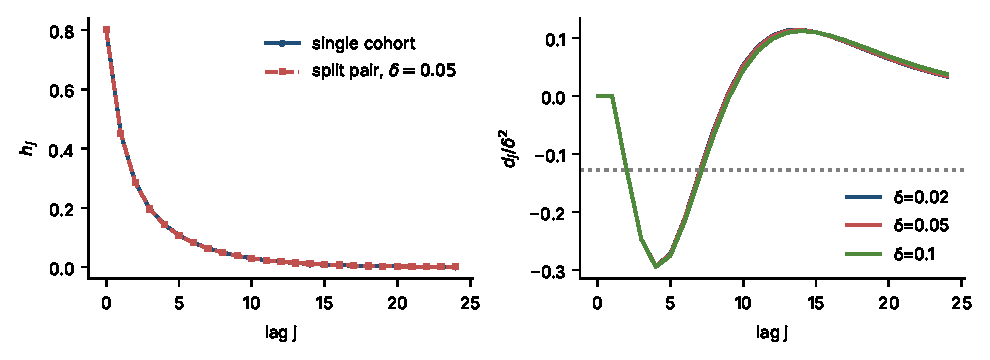
\includegraphics[width=\textwidth]{figs/fig_impulse.pdf}
\caption{Left: impulse responses of the single cohort and the split pair ($\delta=0.05$) are nearly indistinguishable. Right: the difference scaled by $\delta^2$ collapses onto one curve, with first nonzero value $-\kappa^2q$ at lag 2 (dotted). Calibration $a=0.5$, $\kappa=0.8$, $q=0.2$, $\eta=0.4$.}\label{fig:impulse}
\end{figure}

\paragraph{A Monte Carlo check of the exact error.} Formula \eqref{eq:exacterr} is exact for the likelihood-ratio test. We simulated 200,000 noisy paths per hypothesis at the calibration ($\sigma=0.01$, $\delta=0.05$) for several pulse sizes and horizons (Table~\ref{tab:mcerr}); simulated errors match the formula to Monte Carlo precision under both hypotheses.

\begin{table}[t]\centering
\begin{threeparttable}
\caption{Exact known-pair error: formula versus simulation}\label{tab:mcerr}
\begin{tabular}{rrccc}
\toprule
Pulse $V$ & Horizon $T$ & $\Phi(-V\|d_T\|_2/2\sigma)$ & Simulated error, $H_0$ & Simulated error, $H_\delta$\\
\midrule
20 & 3 & 0.3745 & 0.3734 & 0.3762\\
40 & 3 & 0.2611 & 0.2599 & 0.2603\\
40 & 10 & 0.0029 & 0.0030 & 0.0027\\
80 & 20 & $1.8\times10^{-10}$ & 0 & 0\\
\bottomrule
\end{tabular}
\begin{tablenotes}\footnotesize\item 200,000 paths per hypothesis; $a=0.5$, $\kappa=0.8$, $q=0.2$, $\eta=0.4$. \end{tablenotes}
\end{threeparttable}
\end{table}

Figure~\ref{fig:impulse} shows why the problem is hard. The two economies have the same direct impact and the same first-lag response; they first differ at lag two, by an amount proportional to $\delta^2$, and the whole difference sequence scales with $\delta^2$. A test therefore needs the signal-to-noise ratio $V\|d\|/\sigma$ to grow like $\delta^{-2}$, which is the quantity order, and because the adverse mark of a probe grows with the square of its size, capital grows like $\delta^{-4}$.

\subsection{Execution cost}

A probe changes inventory as well as price. We therefore specify cash and execution timing. Price has units of currency per asset, and $\kappa$ currency per squared quantity.

\begin{lemma}[Fair execution]\label{lem:toeplitz}
For a quote schedule refreshed after the uncontrolled state update, execution at the average price of a linear book costs, relative to the constant fundamental mark,
\begin{equation}\label{eq:cost}
C(v)=\tfrac12v^\top T_hv+c\|v\|_1,\qquad (T_h)_{ij}=h_{|i-j|}.
\end{equation}
In the positive stable economy $T_h$ is positive definite, so no nonzero round trip produces a deterministic gain.
\end{lemma}

We verify the ledger identity \eqref{eq:cost} against an explicit cash account to $5.7\times10^{-13}$ on 1,000 random probes, and the smallest eigenvalue of $T_h$ over 1,000 random stable positive economies is $0.141$. A direct-only proxy $\sum\tfrac12\kappa v_t^2$ omits cross-time impact: for $v=(+1,-1)$ it gives $0.80$ against a true Toeplitz loss of $h_0-h_1=0.3488$.

\subsection{Capital supplied by a counterparty}

\begin{theorem}[Sharp robust quantity cap from cash and margin]\label{thm:cap}
Use the positive, stable, reset economy with constant fundamental price $P_*>0$ and no process noise. A designated dealer fills only nonnegative probes $v_t\ge0$ at the average price $P^0_{t+1}+\kappa v_t/2$ of a linear schedule, holds inventory $I_{t+1}=I_t-v_t$ and cash $K_{t+1}=K_t+v_t(P^0_{t+1}+\kappa v_t/2)-cv_t$, starts with equity $B>0$, and must satisfy $\mu|I_t|P_t\le E_t$ at every time. For the robust contract admitting every probe with $\sum_tv_t\le V$, the largest allowance guaranteeing margin is
\begin{equation}\label{eq:VB}
V_B=\frac{2B}{\beta+\sqrt{\beta^2+4(\mu+\tfrac12)\kappa B}},\qquad\beta=c+\mu P_*,
\end{equation}
equivalently $(\mu+\tfrac12)\kappa V^2+(c+\mu P_*)V\le B$. The cap holds across all positive cohort representations with $S<1$, without resolving individual rates. An observer that receives only noisy prices and executed quantities has best error $\Phi[-V_B\|d_T\|_2/(2\sigma)]$ within this allowance; fixed error $\alpha<1/2$ requires capital of order at least $\delta^{-4}$, and a single positive pulse attains that order.
\end{theorem}

Even with zero initial inventory, the probe creates a quadratic adverse mark that a fixed initial price exposure would miss. Figure~\ref{fig:knownpair} illustrates the experiment.

\begin{figure}[t]\centering
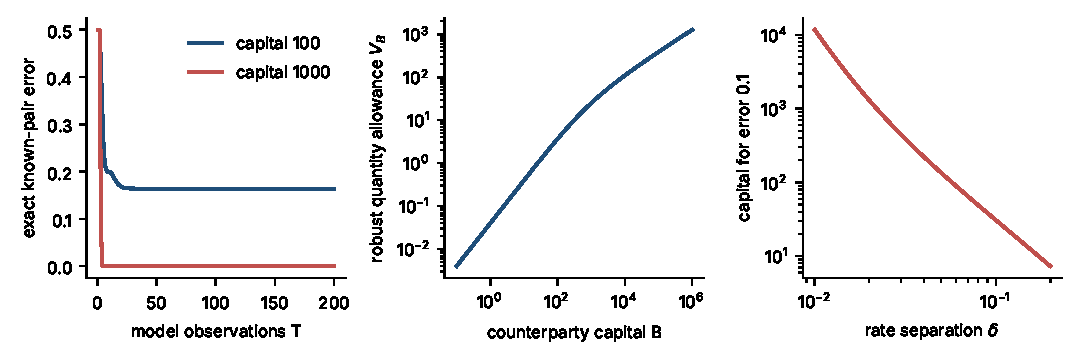
\includegraphics[width=\textwidth]{figs/fig_knownpair.pdf}
\caption{Known-pair experiment funded by the counterparty cash/margin contract. (a) Exact Gaussian error at fixed capital 100 and 1,000, separation $\delta=0.05$. (b) The sharp robust quantity allowance \eqref{eq:VB}. (c) Capital for error $0.1$ with 200 observations. Parameters: $a=0.5$, $\kappa=0.8$, $q=0.2$, $\eta=0.4$, observation s.d.\ $0.003$, reference price 100, margin $0.25$, cost $0.02$. No process noise.}\label{fig:knownpair}
\end{figure}

\begin{proposition}[Exact financial disclosure changes the experiment]\label{prop:disclosure}
In this noiseless-state account, exact disclosure of the third equity mark after a single positive pulse $0<A\le V_B$ distinguishes the known pair with zero error for every $\delta>0$.
\end{proposition}

Exact marked equity is extra information, not a free observation assumed by the price-only theorem. Real account marks have their own precision: with reports rounded to $0.01$, a guaranteed change requires a larger trade (Section~\ref{sec:disclosure}).

\subsection{Capital paid by the probe trader}

\begin{lemma}[Time-domain Toeplitz coercivity: capital order for funded probes]\label{thm:capital}
Use the same economy and execution law. The statistical observer receives only noisy prices and executed quantities. The probe trader starts with cash $B>0$ and zero inventory; a finite signed sequence $v$ changes inventory by $+v_t$ and cash by $K_{t+1}=K_t-v_t(P^0_{t+1}+\kappa v_t/2)-c|v_t|$, after which trading stops and the trader must remain solvent as the price returns to $P_*$. Put
\[
r=1-\epsilon(1-S)<1,\qquad m=\kappa\frac{1-r}{1+r}>0,\qquad K_*=\frac{2\kappa^2q}{\epsilon^3(1-S)^2}.
\]
Every solvent strategy satisfies $\KL(P_0^v\|P_\delta^v)\le K_*^2B\delta^4/(\sigma^2m)$, so error at most $\alpha<1/2$ requires
\begin{equation}\label{eq:Bmin}
B\;\ge\;\frac{2\sigma^2m(1-2\alpha)^2}{K_*^2\delta^4},
\end{equation}
without a quantity cap and at any horizon. Conversely, for any margin fraction $0<\mu\le1$, the pulse $A$ in \eqref{eq:pulse} achieves error $\alpha$ and remains margin-solvent at every later mark with capital $B_A=\tfrac{\kappa}{2}A^2+(c+\mu P_*)A$. Necessary and sufficient capital orders are $\delta^{-4}$.
\end{lemma}

Lemma~\ref{thm:capital} is an order statement: an elementary time-domain coercivity argument for Toeplitz forms that establishes the $\delta^{-4}$ rate before the exact frequency-domain optimization of Section~\ref{sec:account}. Its explicit lower constant is correspondingly loose: at the calibrated parameters it evaluates to $4.9\times10^{-4}$ par units at $\delta=0.05$ with $\epsilon=0.35$, five orders of magnitude below any design we can execute, and because $m/K_*^2\propto\epsilon^7(1-S)^5$ it collapses near the boundary of the family. We therefore state it as a lemma; Section~\ref{sec:account} computes the constant that matters, within 5\% of a feasible design at every separation.

\subsection{A worked example: two Kalman desks}\label{sec:worked}

To make the orders concrete, consider two desks that track the same trend with Kalman filters (Lemma~\ref{lem:micro}(i)) and differ only in their signal-to-noise ratios: $\sigma_\zeta^2/\sigma_\nu^2=0.09$ and $0.16$. Their gains are $\eta_1=0.2584$ and $\eta_2=0.3279$, so $\bar\eta=0.2931$ and $\delta=0.0348$. With equal weights, the economy is observationally the split pair of Theorem~\ref{thm:quantity} around $\bar\eta$, and the response difference first appears at lag two, $d_2=-\kappa^2q\delta^2=-1.55\times10^{-4}$ (verified).

A supervisor who wants to tell this market from a single desk with gain $\bar\eta$ at 5\% error using a single pulse and the third observation needs $A=2\sigma\Phi^{-1}(0.95)/(\kappa^2q\delta^2)=212$ units of executed quantity, and, under a 0.5\% margin and 4 basis points of fees, single-pulse capital of $18{,}166$ par units. The pulse is very inefficient: by the $\delta^{-4}$ scaling of Theorem~\ref{thm:spectral}, the optimal flat probe needs about $61.41\times(0.05/0.0348)^4\approx262$ par units. Converting with the measured Roll noise (factor $(0.40/0.01)^2$), the optimal probe costs roughly $4\times10^5$ USDT and the naive pulse about $3\times10^7$ USDT. Two desks whose signal-to-noise ratios differ by almost a factor of two are therefore expensive, but not impossible, to tell apart by probing; three or more desks are much harder (Theorem~\ref{thm:kcohort}).

\subsection{What prices hide, in economic terms}\label{sec:primitives}

The worked example states the barrier in signal-to-noise ratios. That is the general picture. Write $s=\sigma_\zeta^2/\sigma_\nu^2$ for a desk's signal-to-noise ratio, so that by \eqref{eq:kgain} its memory rate is $1-\eta(s)$ with
\[
\eta(s)=\tfrac12\bigl(\sqrt{s^2+4s}-s\bigr),\qquad \eta'(s)=\tfrac12\Bigl(\frac{s+2}{\sqrt{s^2+4s}}-1\Bigr)>0 ,
\]
and $\eta$ is increasing and concave. With no inventory penalty, the first-order condition of the Remark on exponential memory gives the trading intensity $q_i=\beta_i/\lambda_{{\rm tc},i}$: what the desk expects to earn per unit of belief, over what it pays to trade.

\begin{proposition}[Identification in economic primitives]\label{prop:primitives}
Consider $K$ Kalman desks (Lemma~\ref{lem:micro}(i)) with signal-to-noise ratios $s_i\in[\underline s,\bar s]\subset(0,\infty)$ and intensities $q_i=\beta_i/\lambda_{{\rm tc},i}$, and write $c_-=\eta'(\bar s)$ and $c_+=\eta'(\underline s)$.
\begin{enumerate}[label=(\roman*)]
\item Prices and aggregate order flow depend on the desks only through the measure
\[
\sum_iq_i\,\eta(s_i)\,\delta_{1-\eta(s_i)}.
\]
Desks are identified through their signal-to-noise ratios and intensities only; expected returns and trading costs enter only through their ratio, and two populations with the same intensity-weighted distribution of signal-to-noise ratios are observationally equivalent.
\item Fix a centre $s_c$ and let the ratios lie in $s_c+\Delta s\,[-1,1]\subset[\underline s,\bar s]$. Recovering the intensity-weighted distribution of signal-to-noise ratios to Wasserstein accuracy of order $\Delta s$, or its weights $q_i\eta(s_i)$, from $N$ noisy reset experiments with worst-case error probability below $1/4$ requires $N\ge c\,\sigma^2(\Delta s)^{-(4K-2)}$; on separated configurations, Prony's method of Theorem~\ref{prop:esprit} composed with $\eta^{-1}$ achieves this order. The constants are those of Theorems~\ref{thm:kcohort} and~\ref{prop:esprit} multiplied by powers of $c_-$ and $c_+$.
\end{enumerate}
\end{proposition}

\begin{proof}
(i) By Lemma~\ref{lem:micro}(i) desk $i$ is a cohort with memory rate $1-\eta(s_i)$ and weight $q_i$, so Theorem~\ref{thm:merged} applies, and $\beta_i,\lambda_{{\rm tc},i}$ enter the economy only through $q_i$. (ii) On $[\underline s,\bar s]$, $\eta$ is a $C^1$ bijection onto its image with $c_-\le\eta'\le c_+$. Lower bound: take the two economies of Theorem~\ref{thm:kcohort} with centre $r_c=1-\eta(s_c)$ and rate spacing $\Delta\eta=c_-\Delta s$. By the mean value theorem their gains are images of ratios in $s_c+\Delta s\,[-1,1]$, so they are two populations of Kalman desks in the class, and the bound $N\ge c\,\sigma^2(\Delta\eta)^{-(4K-2)}=c\,c_-^{-(4K-2)}\sigma^2(\Delta s)^{-(4K-2)}$ applies to recovering their weights. Because $\eta$ is $c_+$-Lipschitz, the Wasserstein distance between the two distributions of ratios is at least $1/c_+$ times that between the two distributions of rates, which Theorem~\ref{thm:kcohort} bounds below by a constant times $\Delta\eta=c_-\Delta s$. Upper bound: ratios in $s_c+\Delta s\,[-1,1]$ with spacing at least $\gamma\Delta s$ have gains in $\eta(s_c)+c_+\Delta s\,[-1,1]$ with spacing at least $c_-\gamma\Delta s$, a class of the form required by Theorem~\ref{prop:esprit} with rescaled separation $\gamma c_-/c_+$; Prony's method recovers the rates and weights at that theorem's rate, and $\eta^{-1}$, which is $1/c_-$-Lipschitz, maps rate errors to ratio errors.
\end{proof}

The private information a supervisor would most like to know, how good each desk's information is, is exactly what prices hide. In the worked example the two desks' ratios differ by a factor of almost two, and separating them already costs hundreds of thousands of dollars of probing capital. The proposition takes intensities to vary independently of information quality, because they also reflect costs and capital. The next proposition asks what happens when the economics ties them together.

\begin{proposition}[Intensity tied to information quality]\label{prop:tied}
Let each desk's intensity be a known function of its signal-to-noise ratio, $q=\varphi(s)$ with $\varphi$ positive and $C^2$ on $[\underline s,\bar s]$ (for a mean--variance desk, $\varphi(s)$ increases with $s$), and let $n_i\ge0$ denote the mass of desks with ratio $s_i$ (a divisible population, not an integer desk count). Write $s(\eta)$ for the inverse gain map and $w(\eta)=\varphi(s(\eta))\,\eta$ for the weight per desk as a function of its gain.
\begin{enumerate}[label=(\roman*)]
\item \emph{Unknown numbers of desks.} The merged measure is $\sum_in_i\,w(\eta(s_i))\,\delta_{1-\eta(s_i)}$. Every positive measure with finitely many atoms in $[1-\eta(\bar s),1-\eta(\underline s)]$ is of this form, with $n_i=m_i/w(\eta_i)$ for an atom of mass $m_i$ at $1-\eta_i$. So when the numbers of desks of each type are not known, tying intensity to information quality removes no economy, and every lower bound of Proposition~\ref{prop:primitives}(ii) holds unchanged.
\item \emph{Known numbers of desks.} If the $n_i$ are also known, the set of economies is smaller, but the single-versus-pair problem keeps its order: one type at gain $\bar\eta$ with $2n$ desks and two types at $\bar\eta\pm\delta$ with $n$ desks each have taps that differ by $n\,\delta^2\,\partial_\eta^2[w(\eta)(1-\eta)^m]_{\bar\eta}+o(\delta^2)$, so separating them needs $N\ge c\,\sigma^2\delta^{-4}$ reset experiments, the order the symmetric pair has when intensities vary freely.
\item \emph{Self-confirming configurations.} Suppose the ratio each desk perceives is the one implied by the closed-loop dynamics it trades in, through a map $T$ from configurations $(s_1,\dots,s_K)$ to perceived ratios that is continuous on a box $\prod_i[\underline s,\bar s]$ and maps it into itself. Then a configuration with $T(s)=s$ exists, and parts (i)--(ii) and Proposition~\ref{prop:primitives} apply at it.
\end{enumerate}
\end{proposition}

\begin{proof}
(i) Desk type $i$ is a cohort with gain $\eta_i=\eta(s_i)$, memory rate $1-\eta_i$ and total weight $n_i\varphi(s_i)$, so it contributes $n_i\varphi(s_i)\eta_i=n_iw(\eta_i)$ to the atom at $1-\eta_i$. Since $w>0$, any atom mass $m_i\ge0$ is attained with $n_i=m_i/w(\eta_i)$. (ii) Write $g_m(\eta)=w(\eta)(1-\eta)^m$; the tap difference is $n[g_m(\bar\eta+\delta)+g_m(\bar\eta-\delta)-2g_m(\bar\eta)]=n\delta^2g_m''(\bar\eta)+o(\delta^2)$, with $\sum_m\sup|g_m''|^2<\infty$ on gains bounded away from zero, so the Euclidean distance between the two tap vectors is $O(n\delta^2)$ and the Kullback--Leibler divergence over $N$ experiments is $O(Nn^2\delta^4/\sigma^2)$; Le Cam's two-point argument gives the bound. (iii) is Brouwer's fixed-point theorem.
\end{proof}

So the barrier does not depend on intensities varying freely: it survives any known link between intensity and information quality as long as the supervisor does not also know how many desks of each kind there are, and even then the simplest separation problem keeps its $\delta^{-4}$ order. Whether the full $(\Delta\eta)^{-(4K-2)}$ exponent survives with known numbers of desks is open. Part~(iii) shows only that self-confirming configurations exist under continuity; it does not derive the map $T$ from a model of the desks' learning.

\subsection{Natural excitation and the cost of ambiguity}

Natural price innovations can also separate the pair with zero controlled quantity: an exact finite-sample test on independent three-step blocks needs order $\delta^{-4}$ blocks (Internet Appendix, Proposition~\ref{prop:passive0}), the same order as the passive Whittle bound of Section~\ref{sec:mixtures}. Non-identification also has a price on the quote side: when the relevant set of economies includes costlier ones, a robust dealer widens its quote, which the companion paper analyses \citep{niroula2026b}; cohort non-identification alone does not establish that the worst relevant cost exceeds the informed one.
\section{Account-level capital}\label{sec:account}

Lemma~\ref{thm:capital} gives the order but not the constant. This section computes what a trader actually needs under a calibrated linear-impact environment, then converts it to Bitcoin dollars.

\paragraph{Numerical status.} The analytic inequalities below are conditional mathematical bounds. The displayed decimal optima and brackets are numerical evaluations, not independently outward-certified enclosures of the continuous frequency or angle extrema. A finite grid and a matching archived number do not establish that enclosure; rigorous optimization remains a separate verification obligation.

\subsection{Observation design and the tri-region partition}
Under observation horizon $T$ per pulse, $(\delta,B)$ space splits into three regions: a feasible single-pulse region ($C^*=\Theta(\delta^{-4})$ for symmetric splitting), a sequential bounded-probing region where each capped pulse supplies divergence $V_{\rm eff}^2\|d_T\|_2^2/(2\sigma^2)$, and an infeasible region below the finite-session resolution floor $\delta_{\min}=\Theta(T_{\rm session}^{-1/4})$ (Supplemental Appendix, Proposition~\ref{prop:tri} and Figure~\ref{fig:phase}).

\subsection{Account-level capital and the gap to the lower bound}

We run each candidate design through an explicit synthetic ledger at reference price $P_*=100$: fills at the average linear-book price, taker fees of 4 basis points, marks at the prevailing price, and 0.5\% maintenance margin. Initial capital is $C_0=\max_t({\rm margin}_t-{\rm equity}_t)$, maximized over both hypotheses, and the test uses the full price path including unwind legs.

\begin{table}[t]\centering\small
\begin{threeparttable}
\caption{Account-level initial capital at $\delta=0.05$ (par units)}\label{tab:ledger}
\setlength{\tabcolsep}{4pt}
\begin{tabular}{lrrrrrr}
\toprule
Design & $C_0$ & Error & End inv. & Peak margin & Max $|v_t|$ & Trades\\
\midrule
12 buys, $T=20$ apart, never unwound & 229.13 & 0.0578 & 75.00 & 39.38 & 6.25 & 12\\
6 buy/sell round trips & 189.45 & 0.0308 & 0.00 & 3.28 & 6.25 & 12\\
5 buy/sell round trips & 157.89 & 0.0442 & 0.00 & 3.28 & 6.25 & 10\\
12 buys, each unwound after 20 steps & 378.82 & 0.0040 & 0.00 & 3.28 & 6.25 & 24\\
Generalized-eigenvector probe ($L=120$) & 65.06 & 0.0500 & 0.00 & 2.74 & 1.24 & 120\\
Generalized-eigenvector probe ($L=160$) & 64.86 & 0.0500 & 0.00 & 2.17 & 1.09 & 160\\
Fee-refined probe ($L=240$) & 64.48 & 0.0500 & 0.00 & --- & 1.30 & 240\\
\bottomrule
\end{tabular}
\begin{tablenotes}\footnotesize\item The pulse designs place a pulse every 40 steps and close it 20 steps later; the fee-refined probe is re-optimized by sequential quadratic programming over $L=240$. The numerically evaluated lower bound of Theorem~\ref{thm:spectral} is 61.41; the explicit constant of Lemma~\ref{thm:capital} is $4.9\times10^{-4}$.\end{tablenotes}
\end{threeparttable}
\end{table}

Table~\ref{tab:ledger} gives three conclusions. First, twelve buys that are never unwound fail the 5\% target once the test uses the joint price path (divergence $4.95<5.41$) and end with 75 units of inventory. Second, if every unwind leg is itself informative, five or six round trips meet the target with zero terminal inventory. Third, pulses are not optimal: a generalized-eigenvector probe, which maximizes divergence per unit of fee-free round-trip cost, needs about 65 par units with maximum trade 1.25 and maximum displacement 2.23, well inside limits.

For flat fee-paying policies $v\in\R^L$ with $\sum_tv_t=0$, the capital problem is
\begin{equation}\label{eq:capprob}
\min_v\ \max_{i\in\{0,1\}}L_i(v)+\sum_t\phi P_*|v_t|+\max_t\mu P_*|I_t|\quad\text{s.t.}\quad\|(H_1-H_0)v\|_2\ge2\sigma z_{1-\alpha},
\end{equation}
where $L_i(v)=\tfrac12v^\top T_{h_i}v$ is the exact Toeplitz round-trip loss. Zero-padding embeds horizon $L$ into $L+1$ at identical cost and information, so the minimum is non-increasing in $L$.

\begin{theorem}[Spectral dissipation lower bound]\label{thm:spectral}
Let $\hat H_i(z)=\sum_{j\ge0}h_{i,j}z^{-j}$, $\Delta\hat H=\hat H_1-\hat H_0$, and define the dissipation kernel
\begin{equation}\label{eq:gdiss}
g_i(\omega)=\mathrm{Re}\,\hat H_i(e^{i\omega})-\kappa/2>0\qquad\forall\omega\in[-\pi,\pi].
\end{equation}
\begin{enumerate}[label=(\roman*)]
\item \emph{Toeplitz energy identity.} For any flat round trip, $L_i(v)=\frac1{2\pi}\int_{-\pi}^{\pi}g_i(\omega)|V(e^{i\omega})|^2d\omega$.
\item \emph{Lower bound.} $\|(H_1-H_0)v\|_2^2\le\sup_\omega\frac{|\Delta\hat H(e^{i\omega})|^2}{g_i(\omega)}L_i(v)$, so every deterministic round trip with error at most $\alpha$ has
\begin{equation}\label{eq:Cdet}
L_i(v)\;\ge\;4\sigma^2z_{1-\alpha}^2\inf_\omega\frac{g_i(\omega)}{|\Delta\hat H(e^{i\omega})|^2}\;\equiv\;C^*_{\rm det,quad}(\delta).
\end{equation}
\item \emph{Bracket.} At $\delta=0.05$, $C^*_{\rm det,quad}=61.14$ at $\omega^*=0.2526$; adding the unavoidable fee $\phi P_*\cdot2\sigma z/\sup_\omega|\Delta\hat H|$ gives the numerical lower estimate $C_{\rm det}\ge61.41$. A feasible 240-step sequence attains 64.48, so the fee-paying optimum lies in $[61.41,64.48]$.
\item \emph{Process noise.} Let the price also receive the innovations $w_t\sim N(0,\sigma_w^2)$ of \eqref{eq:price}, independent of observation noise $\nu_t\sim N(0,\sigma_\nu^2)$, so that from the reset state the observer sees $\tilde x_t=(h_i*v)_t+\kappa^{-1}(h_i*w)_t+\nu_t$, $t<T$. For the known pair of Theorem~\ref{thm:quantity}, put $\sigma_{\rm eff}^2=\sigma_\nu^2+\sigma_w^2/4$, $\bar M=1/(1-S)$ and $C_w=2\sigma_w^4\bar M^2K_*^2(\sigma_\nu^2+\sigma_w^2\bar M^2)/(\kappa^2\sigma_\nu^2\sigma_{\rm eff}^4)$. Every deterministic round trip whose test has errors $\alpha$ and $\beta$ under the two hypotheses satisfies
\begin{equation}\label{eq:Cnoise}
L_i(v)\;\ge\;2\sigma_{\rm eff}^2\bigl[{\rm kl}(\alpha,1-\beta)-C_wT\delta^4\bigr]_+\inf_\omega\frac{g_i(\omega)}{|\Delta\hat H(e^{i\omega})|^2},
\end{equation}
with ${\rm kl}$ as in Theorem~\ref{thm:adaptive}. In-loop noise therefore leaves the $\delta^{-4}$ capital order intact for every horizon $T\le{\rm kl}(\alpha,1-\beta)/(2C_w\delta^4)$; at horizons of order $\delta^{-4}$ and longer, the noise itself separates the pair without a probe (Theorem~\ref{prop:passive}).
\end{enumerate}
\end{theorem}

\begin{figure}[t]\centering
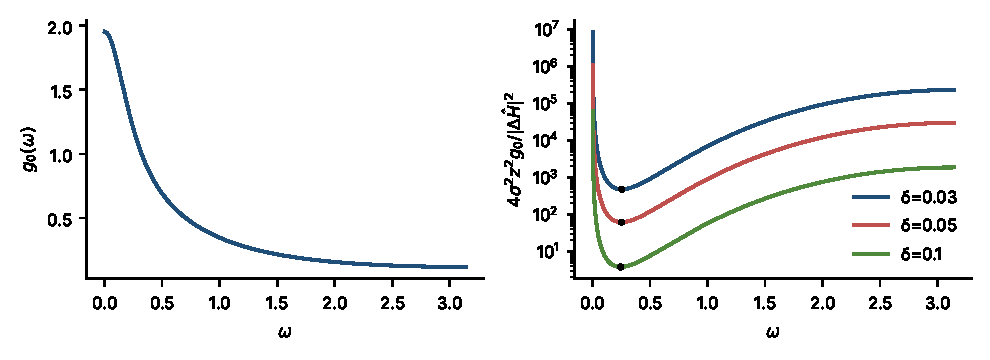
\includegraphics[width=\textwidth]{figs/fig_dissipation.pdf}
\caption{Left: the dissipation kernel $g_0(\omega)$ is strictly positive. Right: the capital ratio in \eqref{eq:Cdet}; dots mark its minimum, near $\omega^*\approx0.25$ for every separation. Recomputed in this revision.}\label{fig:dissip}
\end{figure}

Positivity of $g_i$ follows from Lemma~\ref{lem:cm}: $g_i(\omega)=\tfrac12\sum_\ell\omega_\ell\frac{1-\lambda_\ell^2}{1-2\lambda_\ell\cos\omega+\lambda_\ell^2}>0$. We compute $C^*_{\rm det,quad}$ across separations (Table~\ref{tab:capbounds}): $61.14$ at $\delta=0.05$, with $\delta^4C^*_{\rm det,quad}$ between $3.67\times10^{-4}$ and $3.84\times10^{-4}$, confirming the $\delta^{-4}$ law. The fee term, the feasible upper bounds and the adaptive bound of Theorem~\ref{thm:adaptive} are reported in the same table.

\begin{theorem}[Adaptive and sequential probing]\label{thm:adaptive}
Let $(v_t)_{t\le\tau}$ be any non-anticipating policy adapted to the price filtration, with an almost surely finite stopping time and $\sum_{t\le\tau}v_t=0$. Then
\begin{equation}\label{eq:adaptive}
\E_0[L_0(v)]\;\ge\;2\sigma^2\,{\rm kl}(\alpha,1-\beta)\inf_\omega\frac{g_0(\omega)}{|\Delta\hat H(e^{i\omega})|^2},
\end{equation}
where ${\rm kl}(\alpha,1-\beta)=\alpha\log\tfrac{\alpha}{1-\beta}+(1-\alpha)\log\tfrac{1-\alpha}{\beta}$.
Hence adaptation can lower expected fee-free loss by at most the factor ${\rm kl}(\alpha,1-\beta)/(2z_{1-\alpha}^2)\approx0.4897$ at $\alpha=\beta=0.05$, and cannot alter the $\delta^{-4}$ order.
\end{theorem}

At $\delta=0.05$ the adaptive bound is $29.94$, or $30.22$ with the minimal fee. Pairing it with the feasible deterministic 64.48 gives a numerical ratio of at least $0.464$. In 20{,}000 simulated sequential probability-ratio tests, which split the optimal probe into ten copies of equal information, mean loss was $39.5$ under $H_0$, between the two bounds, but losses vary with the stopping time: the 95th and 99th percentiles of required account capital were $91.7$ and $128.4$, and funding a trader with only the mean loss gives a 37.5\% insolvency rate before the test ends. Expected-loss savings are not solvency savings.

\begin{table}[t]\centering\small
\begin{threeparttable}
\caption{Capital lower bounds and feasible upper bounds across separations (par units)}\label{tab:capbounds}
\begin{tabular}{lcccccc}
\toprule
$\delta$ & $\omega^*$ & $C^*_{\rm det,quad}$ & $\delta^4C^*_{\rm det,quad}$ & Certified $C_{\rm det}$ & Feasible UB & Adaptive LB\\
\midrule
0.02 & 0.2546 & 2397.85 & $3.84\times10^{-4}$ & 2399.58 & 2428.25 & 1176.04\\
0.03 & 0.2541 & 473.19 & $3.83\times10^{-4}$ & 473.97 & 484.50 & 232.51\\
0.05 & 0.2526 & 61.14 & $3.82\times10^{-4}$ & 61.41 & 64.48 & 30.22\\
0.08 & 0.2488 & 9.26 & $3.79\times10^{-4}$ & 9.37 & 10.38 & 4.64\\
0.10 & 0.2453 & 3.77 & $3.77\times10^{-4}$ & 3.83 & 4.44 & 1.91\\
0.15 & 0.2331 & 0.73 & $3.67\times10^{-4}$ & 0.76 & 1.01 & 0.38\\
\bottomrule
\end{tabular}
\begin{tablenotes}\footnotesize\item Calibration $a=0.5$, $\kappa=0.8$, $q=0.2$, $\eta=0.4$, $\sigma=0.01$, $\alpha=0.05$. From \texttt{recompute\_theory.py} and \texttt{recompute\_p1\_capital.py}; the numerical-bound column adds the fee lower bound to the fee-free infimum; the feasible column is the best flat probe found over $L\le240$; the adaptive column adds the fee lower bound to the adaptive bound.\end{tablenotes}
\end{threeparttable}
\end{table}

\begin{theorem}[Finite-horizon Rayleigh--H\"older duality]\label{thm:rh}
For a horizon of $L\ge4$ trading periods, let $E\in\R^{L\times(L-1)}$ be the first-difference basis of flat probes ($\sum_tv_t=0$), $Q_i=\tfrac12T_{h_i}$ (so that $L_i(v)=v^\top Q_iv$), $A_{\rm diff}=(H_1-H_0)^\top(H_1-H_0)$, and let $G_i=E^\top Q_iE\succ0$ and $M=E^\top A_{\rm diff}E\succeq0$ be the reduced execution-loss and information matrices, with $G_i$-orthonormal generalized eigenvectors $e_j$ and eigenvalues $0\le\lambda_1\le\cdots\le\lambda_{L-3}<\lambda_{L-2}\le\lambda_{L-1}$; put $c_{\rm req}=4\sigma^2z_{1-\alpha}^2$ and $c_{\rm fee}=\phi P_*$. For $\theta\in[0,\pi)$ let $d(\theta)=\cos\theta\,e_{L-2}+\sin\theta\,e_{L-1}$, $\lambda(\theta)=\lambda_{L-2}\cos^2\theta+\lambda_{L-1}\sin^2\theta$, $s_\theta={\rm sign}(Ed(\theta))$, and
\begin{equation}\label{eq:rhdefs}
\begin{gathered}
F_{\rm dom}(\theta)=c_{\rm fee}\sqrt{\frac{c_{\rm req}}{\lambda(\theta)}}\,\|Ed(\theta)\|_1,\qquad W_\perp(\theta)=c_{\rm fee}^2\sum_{j\le L-3}\frac{(s_\theta^\top Ee_j)^2}{1-\lambda_j/\lambda(\theta)},\\
\gamma(\theta)=\frac{\lambda(\theta)\,\lambda_{L-3}}{(\lambda(\theta)-\lambda_{L-3})\,c_{\rm req}} .
\end{gathered}
\end{equation}
Then every flat probe meeting the separation constraint of \eqref{eq:capprob} satisfies
\begin{equation}\label{eq:rh}
L_i(v)+c_{\rm fee}\|v\|_1\;\ge\;\min_{\theta}\Bigl\{\frac{c_{\rm req}}{\lambda(\theta)}+\Psi(\theta)\Bigr\}\;\equiv\;C_{\rm RH}(L)\;\ge\;\frac{c_{\rm req}}{\lambda_{L-1}},
\end{equation}
\[
\Psi(\theta)=\min_{x\ge0}\Bigl\{x^2+\Bigl[F_{\rm dom}(\theta)\bigl(1-\gamma(\theta)x^2\bigr)_+-\sqrt{W_\perp(\theta)}\,x\Bigr]_+\Bigr\}\;\ge0 ,
\]
a piecewise-quadratic minimization in closed form; when $\gamma F_{\rm dom}<1$ and the minimizer has $\gamma x^2\le1$, $\Psi=\max\bigl(0,F_{\rm dom}-W_\perp/(4(1-\gamma F_{\rm dom}))\bigr)$.
\end{theorem}

The bound is computable for any horizon. Table~\ref{tab:rh} reports its quadratic part $c_{\rm req}/\lambda_{L-1}$, which decays toward the infinite-horizon value 61.14 at rate $O(L^{-1})$, the full bound $C_{\rm RH}(L)$, and the best feasible fee-paying probe we find at each horizon. At $L=80$ the full bound is $64.72$ against a best probe of $64.76$ on the same loss-plus-fee objective, so the dual is essentially tight at short horizons; at longer horizons the fee term of the dual weakens and the bracket widens to about 5\%. The fee of unpadded full-support eigenvectors grows as $\Theta(\sqrt L)$, which is why zero-padded or $L_1$-localized probes are needed at long horizons.

\begin{table}[t]\centering\small
\begin{threeparttable}
\caption{Finite-horizon capital at $\delta=0.05$ (par units)}\label{tab:rh}
\setlength{\tabcolsep}{4pt}
\begin{tabular}{lcccc}
\toprule
Horizon $L$ & Quadratic part $c_{\rm req}/\lambda_{L-1}$ & Full bound $C_{\rm RH}(L)$ & Best feasible probe & Gap to $C_{\rm det}=61.41$\\
\midrule
80 & 62.55 & 64.72 & 65.02 & 5.9\%\\
120 & 61.84 & 63.39 & 64.59 & 5.2\%\\
160 & 61.54 & 62.46 & 64.50 & 5.0\%\\
240 & 61.32 & 61.76 & 64.48 & 5.0\%\\
320 & 61.25 & --- & $\le64.48$ & $\le5.0\%$\\
480 & 61.19 & --- & $\le64.48$ & $\le5.0\%$\\
\bottomrule
\end{tabular}
\begin{tablenotes}\footnotesize\item Quadratic bound $c_{\rm req}/\lambda_L$ from the generalized eigenproblem of Theorem~\ref{thm:rh} on flat probes (equivalently $c_{\rm req}/(2\lambda'_L)$ with $\lambda'$ computed against $T_{h_0}$ rather than $\tfrac12T_{h_0}$); it converges to the infinite-horizon value 61.14. The full bound minimizes \eqref{eq:rh} over 3{,}600 values of $\theta$ (\texttt{hardening/rh\_bound.py}); at $L=80$ and $120$ a direct numerical minimization of loss plus fee under the separation constraint gives $64.76$ and $64.43$, above the bound. Feasible probes: top generalized eigenvector refined by sequential quadratic programming on the full ledger; at $L=320$ and $480$ the $L=240$ probe padded with zeros is feasible at the same cost, so the best feasible value can only be lower. \end{tablenotes}
\end{threeparttable}
\end{table}

\subsection{Robustness: heteroskedastic impact and probing protocols}
Probing-induced heteroskedasticity and convex impact leave the $\delta^{-4}$ capital order unchanged (Supplemental Appendix, Corollary~\ref{cor:garch}), and four simulated probing protocols all exhibit log--log capital slopes near $-4$ (Table~\ref{tab:protocols}).

\subsection{From par units to Bitcoin dollars}\label{sec:dollars}

Capital scales as $\sigma^2\delta^{-4}$, so the dollar magnitude hinges on the observation noise. Treating the 4 USDT ten-second price volatility as observation noise would give 9.8 million USDT at $\delta=0.05$, but that conflates price volatility with measurement error. We now estimate observation noise from Binance BTCUSDT one-second closes on January 10--20, 2023, with the Roll covariance estimator $\hat\sigma=\sqrt{-{\rm cov}(\Delta p_t,\Delta p_{t-1})}$ \citep{roll1984}. Daily estimates range from $0.09$ to $0.77$ USDT, median $0.40$ USDT.

\begin{table}[t]\centering
\begin{threeparttable}
\caption{Capital lower bound under alternative observation-noise calibrations (USDT)}\label{tab:capital}
\begin{tabular}{lrrr}
\toprule
Noise calibration & $\delta=0.02$ & $\delta=0.05$ & $\delta=0.10$\\
\midrule
Roll estimator, median (0.40 USDT) & 3{,}874{,}696 & 99{,}193 & 6{,}200\\
One-second price-change s.d., median (1.98 USDT) & 93{,}688{,}369 & 2{,}398{,}422 & 149{,}902\\
Earlier assumption (4 USDT, upper scenario) & 383{,}812{,}500 & 9{,}825{,}600 & 614{,}100\\
\bottomrule
\end{tabular}
\begin{tablenotes}\footnotesize
\item $C(\sigma,\delta)=61.41\times(\sigma/0.01)^2\times(0.05/\delta)^4$, with $\sigma$ the unrounded median. Noise estimated on 11 days of checksum-verified Binance BTCUSDT one-second klines. \end{tablenotes}
\end{threeparttable}
\end{table}

\begin{table}[t]\centering\small
\begin{threeparttable}
\caption{Daily observation-noise estimates, Binance BTCUSDT one-second closes}\label{tab:roll}
\begin{tabular}{lccc}
\toprule
Date & Roll $\hat\sigma$ (USDT) & One-second change s.d.\ (USDT) & Mean price (USDT)\\
\midrule
2023-01-10 & 0.152 & 0.679 & 17{,}288\\
2023-01-11 & 0.092 & 0.891 & 17{,}456\\
2023-01-12 & 0.232 & 2.292 & 18{,}343\\
2023-01-13 & 0.348 & 1.762 & 19{,}075\\
2023-01-14 & 0.773 & 3.511 & 20{,}818\\
2023-01-15 & 0.482 & 1.790 & 20{,}778\\
2023-01-16 & 0.629 & 2.357 & 21{,}036\\
2023-01-17 & 0.457 & 1.976 & 21{,}194\\
2023-01-18 & 0.695 & 2.541 & 21{,}122\\
2023-01-19 & 0.402 & 1.316 & 20{,}850\\
2023-01-20 & 0.316 & 2.038 & 21{,}306\\
\midrule
Median & 0.402 & 1.976 & \\
\bottomrule
\end{tabular}
\begin{tablenotes}\footnotesize\item The Roll estimator measures the negative first-order autocovariance of price changes, which reflects bid-ask bounce and recording noise rather than price volatility.\end{tablenotes}
\end{threeparttable}
\end{table}

\begin{figure}[t]\centering
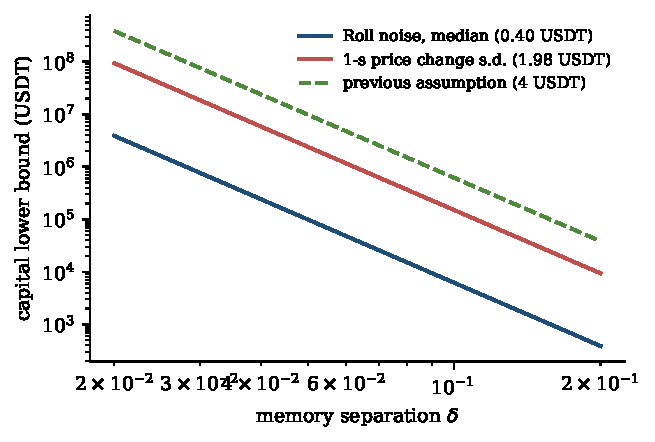
\includegraphics[width=0.62\textwidth]{figs/fig_capital.pdf}
\caption{Capital lower bound against memory separation for three observation-noise calibrations.}\label{fig:capital}
\end{figure}

At realistic noise, separating rates that differ by $0.05$ costs about $9.9\times10^4$ USDT, which is not prohibitive for a well-capitalized desk (Table~\ref{tab:capital}). The barrier becomes large only for finer separation ($3.9$ million USDT at $\delta=0.02$) and, through Theorem~\ref{thm:kcohort}, when several cohorts are unknown. Two factors we do not model would raise these figures: walking several levels of a real book costs more than the linear top-of-book impact assumed here, and impact-induced heteroskedasticity raises the noise a probe must overcome. The capital figures are therefore lower bounds for the stated model.
\section{Unknown mixtures and passive data}\label{sec:mixtures}

Theorem~\ref{thm:quantity} concerns a \emph{known} pair. A supervisor faces an unknown number of cohorts with unknown rates and weights. This section asks how fast the cost of recovering them grows.

\subsection{Why naive pole fitting fails}

Because the memory rates are zeros of $H$ (Theorem~\ref{thm:merged}), extracting poles directly from the price impulse response by matrix-pencil or Prony methods targets closed-loop eigenvalues. A four-step inversion repairs this: (1) decouple $g_t=h_{t+1}-ah_t$; (2) form a Hankel matrix of $g$ and compute a minimal realization by Kung's eigensystem realization; (3) compute its transmission zeros, which are the roots of the denominator of $G$; (4) project reconstructed flow onto the recovered memory filters to obtain the weights (Appendix~\ref{app:era}). Without noise this recovers $K=0$, $K=1$ and well-separated two-cohort systems exactly (Appendix~\ref{app:era}); with noise, per-cohort weights become unreliable once rates are close. The reason is information-theoretic, as the rest of this section shows.

\subsection{Local information: the Cram\'er--Rao benchmark}

\begin{proposition}[Cram\'er--Rao benchmark]\label{prop:crb}
Let $\theta$ collect the weights $w_1,\ldots,w_K$ and rates $\eta_1,\ldots,\eta_K$. Suppose the impulse response $h_t(\theta)$, $t\le T$, is observed with i.i.d.\ Gaussian error from $N$ reset probes of size $V_{\rm probe}$ against innovation noise $\sigma_p$, so the error has standard deviation $\sigma_h=\sigma_p/(V_{\rm probe}\sqrt N)$. With Jacobian $J_{tj}=\partial h_t/\partial\theta_j$ and $F_{\rm unit}=J^\top J$, any regular unbiased estimator has ${\rm Var}(\hat w_k)\ge\sigma_h^2[F_{\rm unit}^{-1}]_{kk}$, and a 95\% interval of half-width ${\rm tol}$ requires
\begin{equation}\label{eq:Ncrb}
N^*\ge\Bigl(\frac{1.96}{\rm tol}\Bigr)^2\Bigl(\frac{\sigma_p}{V_{\rm probe}}\Bigr)^2[F_{\rm unit}^{-1}]_{kk}.
\end{equation}
For $K=2$ with spacing $\Delta\eta$, $[F_{\rm unit}^{-1}]_{kk}=\Theta((\Delta\eta)^{-6})$, so $N^*=\Theta((\Delta\eta)^{-6})$.
\end{proposition}

\begin{table}[t]\centering\small
\begin{threeparttable}
\caption{Cram\'er--Rao sample sizes for multi-cohort weight recovery ($T=120$ taps)}\label{tab:crb}
\begin{tabular}{lcrccc}
\toprule
Scenario & $K$ & $N^*$ probes & $\sigma_{\rm crit}$ & ML success ($f=1$) & RMSE/CRB\\
\midrule
$\eta=0.30$ & 1 & 0.1 & $6.05\times10^{-3}$ & 94\% & 1.02\\
$\Delta\eta=0.30$ & 2 & 47.8 & $2.31\times10^{-4}$ & 94\% & 1.01\\
$\Delta\eta=0.20$ & 2 & 597 & $6.55\times10^{-5}$ & 96\% & 0.98\\
$\Delta\eta=0.10$ ($\delta=0.05$ pair) & 2 & 40{,}374 & $7.96\times10^{-6}$ & 93\% & 1.03\\
$\Delta\eta=0.05$ & 2 & 2{,}620{,}320 & $9.88\times10^{-7}$ & 95\% & 1.03\\
spacing 0.10 & 3 & 17{,}349{,}791 & $3.84\times10^{-7}$ & 98\% & 1.22\\
spacing 0.20 & 3 & 27{,}038 & $9.73\times10^{-6}$ & 98\% & 0.88\\
\bottomrule
\end{tabular}
\begin{tablenotes}\footnotesize\item Tolerance $\pm0.01$ at 95\%. $\sigma_{\rm crit}$ is the single-probe noise at which one probe suffices; operational single-probe noise is $1.6\times10^{-3}$. ML columns: least squares over all weights and rates from six generic starts (never the true values), 200 replications per row at $\sigma_{\rm crit}$; success means every weight within $\pm0.01$. Fitted log--log slope of $N^*$ in $\Delta\eta$: $-6.04$. \end{tablenotes}
\end{threeparttable}
\end{table}

At the critical noise level maximum likelihood attains the bound: its RMSE for the hardest weight is between 0.88 and 1.22 times the Cram\'er--Rao value and every weight is within tolerance in 93\% to 98\% of replications (Table~\ref{tab:crb}), so the critical noise levels, not estimator failure, are what make close cohorts expensive. Under ordinary surveillance budgets ($N\le50$) unbiased estimators cannot resolve close weights.

\subsection{A global two-point bound for any estimator}

Proposition~\ref{prop:crb} applies to regular unbiased estimators. Could biased, ridge, shrinkage or Bayesian estimators escape the $(\Delta\eta)^{-6}$ scaling? No.

\begin{theorem}[Global two-point bound and matching upper bound, $K=2$]\label{thm:twocohort}
Fix total weight $q=0.20$, mean rate $\bar\eta=0.40$, target weight separation $\tau=0.01$, and $\Delta\eta\in(0,8/11)$. Let $p_\mp=\tfrac12\mp\tau/q$ and
\begin{equation}\label{eq:pair}
\theta_0=(qp_-,qp_+,\bar\eta-p_+\Delta\eta,\bar\eta+p_-\Delta\eta),\qquad\theta_1=(qp_+,qp_-,\bar\eta-p_-\Delta\eta,\bar\eta+p_+\Delta\eta).
\end{equation}
\begin{enumerate}[label=(\roman*)]
\item Label cohorts in increasing order of rate, so that weight vectors are compared rate by rate (as unordered sets the two weight vectors coincide). Both economies have spacing $\Delta\eta$, weight separation $\|w(\theta_1)-w(\theta_0)\|_\infty=2\tau$ in this labelling, and equal rate moments $M_m=\sum_kw_k\eta_k^m$ for $m\in\{0,1,2\}$, while
\begin{equation}\label{eq:dM3}
M_3(\theta_1)-M_3(\theta_0)=4\tau p_-p_+(\Delta\eta)^3 .
\end{equation}
Hence $\|h(\theta_1)-h(\theta_0)\|_2=\Theta(\tau(\Delta\eta)^3)$.
\item For any measurable estimator (including biased, ridge, James--Stein or MAP) that reports weights in the same rate order, the supremum being over the class of two-cohort economies with total weight $q$, mean rate $\bar\eta$ and spacing $\Delta\eta$,
\begin{equation}\label{eq:lecam2}
\sup_\theta P_\theta(\|\hat w-w(\theta)\|_\infty\ge\tau)\;\ge\;1-\Phi\!\Bigl(\frac{\sqrt N\|h(\theta_1)-h(\theta_0)\|_2}{2\sigma_h}\Bigr),
\end{equation}
so failure probability at most $0.05$ requires $N\ge4\sigma_h^2z_{0.95}^2/\|h(\theta_1)-h(\theta_0)\|_2^2=\Omega((\Delta\eta)^{-6})$. The same bound holds without any labelling convention for the permutation-invariant loss
\[
d_\infty(\hat\theta,\theta)=\min_{\pi\in S_2}\max_{k}\bigl(|\hat w_{\pi(k)}-w_k|+|\hat\eta_{\pi(k)}-\eta_k|\bigr)
\]
in place of $\|\hat w-w(\theta)\|_\infty$, whenever $\Delta\eta\ge2\tau q/(q+2\tau)$, because then $d_\infty(\theta_0,\theta_1)=\min\{2\tau(1+\Delta\eta/q),\,(1+2\tau/q)\Delta\eta\}\ge2\tau$.
\item Conversely, on the known-midpoint family a linear estimator that projects the averaged impulse response on the normalized third-moment direction and inverts \eqref{eq:dM3} has error at most $|\hat M_3-M_3|/(2p_-p_+(\Delta\eta)^3)$, giving $N=O(\tau^{-2}(\Delta\eta)^{-6}\log(1/\delta_{\rm fail}))$. On the separated class with weights and rates bounded away from the boundary, Toeplitz deconvolution followed by a Prony--Hankel root step has Hankel determinant $g_1g_3-g_2^2=w_1w_2\eta_1\eta_2r_1r_2(\Delta\eta)^2>0$ for the deconvolved kernel $g_m=\sum_iw_i\eta_ir_i^m$, and perturbation analysis gives the same order.
\end{enumerate}
\end{theorem}

We recomputed the two-point quantities exactly (Table~\ref{tab:lecam}): the moment gap equals $4\tau p_-p_+(\Delta\eta)^3$ to machine precision, and the Le Cam requirement at $\Delta\eta=0.10$ is $5{,}927.6$ resets. The worst-case failure rates of four re-implemented estimators all lie above the lower bound (Table~\ref{tab:lecam}).

\begin{table}[t]\centering\small
\begin{threeparttable}
\caption{Two-point sample complexity for two-cohort weight recovery}\label{tab:lecam}
\begin{tabular}{lcccc}
\toprule
$\Delta\eta$ & $\Delta M_3$ & $\|\Delta h\|_2$ & $N^*_{\rm LeCam}$ (95\%) & $N^*_{\rm CRB}$\\
\midrule
0.30 & $2.67\times10^{-4}$ & $1.98\times10^{-3}$ & 7.1 & 47.8\\
0.20 & $7.92\times10^{-5}$ & $5.60\times10^{-4}$ & 88.2 & 597.0\\
0.14 & $2.72\times10^{-5}$ & $1.89\times10^{-4}$ & 775.3 & 5{,}267.9\\
0.10 & $9.90\times10^{-6}$ & $6.84\times10^{-5}$ & 5{,}927.6 & 40{,}374.2\\
0.08 & $5.07\times10^{-6}$ & $3.49\times10^{-5}$ & 22{,}740.5 & 155{,}048.9\\
0.06 & $2.14\times10^{-6}$ & $1.47\times10^{-5}$ & 128{,}333.0 & 875{,}732.3\\
0.05 & $1.24\times10^{-6}$ & $8.50\times10^{-6}$ & 383{,}859.1 & 2{,}620{,}321.2\\
0.04 & $6.34\times10^{-7}$ & $4.35\times10^{-6}$ & 1{,}466{,}361.5 & 10{,}012{,}662.4\\
\midrule
\multicolumn{5}{p{0.85\textwidth}}{\emph{Worst-case failure at $\Delta\eta=0.10$, $N=50$, 1,000 trials per hypothesis}: bound 44.1\%; ML 94.5\%, ridge 47.5\%, positive-part shrinkage 100\%, heavy prior 73.9\%.}\\
\bottomrule
\end{tabular}
\begin{tablenotes}\footnotesize\item $\tau=0.01$, $\sigma_h=1.6\times10^{-3}$, $a=0.5$, $\kappa=0.8$, 121 taps. Recomputed columns from \texttt{recompute\_theory.py}. Estimators re-implemented in \texttt{recompute\_p1\_estimators.py}: ML is least squares from four starts; ridge and heavy prior are posterior modes with prior standard deviations $(0.05,0.10)$ and $(0.005,0.02)$ for (weights, rates) around the symmetric centre of the two hypotheses; positive-part shrinkage pulls the ML weights toward their mean. Failure means some weight is off by at least $\tau$.\end{tablenotes}
\end{threeparttable}
\end{table}

\begin{remark}[The hard directions carry no risk]\label{rem:riskneutral}
The two economies of Theorem~\ref{thm:twocohort} have the same total weight $\sum_iq_i=q$, so their summed price response $\sum_th_t=\kappa/(1-a-\kappa\sum_iq_i)$ is identical, $2.353$ at the calibration of Table~\ref{tab:lecam}: the directions in which prices are least informative about the cohorts are directions in which cumulative price risk does not move. The summed response is a linear functional of the response and is estimated at the parametric rate whatever the spacing of the memories; the companion paper turns this into a certification theorem, a minimax-optimal pre-trade guard and a decision value of disclosure \citep{niroula2026b}. Identification and safety ask different questions of the same data.
\end{remark}

\subsection{Many unknown cohorts}

\begin{theorem}[$K$-cohort two-point lower bound]\label{thm:kcohort}
Fix $K\ge2$, a center $r_c\in(0,1)$ and total merged weight $W>0$. There exist two $K$-cohort economies with rates in $r_c+\Delta\eta[-1,1]$, positive weights, and merged measures whose moments of order $0,\ldots,2K-2$ coincide while the moment of order $2K-1$ differs by a constant times $(\Delta\eta)^{2K-1}$. Their impulse responses differ by $\|h^A-h^B\|_2\asymp(\Delta\eta)^{2K-1}$, so recovering the weights from $N$ independent noisy reset experiments with worst-case error probability below $1/4$ requires
\[
N\;\ge\;c\,\sigma^2(\Delta\eta)^{-(4K-2)} .
\]
The same requirement holds for the permutation-invariant loss $W_1(\hat M,M)$ between estimated and true merged measures at accuracy $c_KW\Delta\eta$, where $2c_K>0$ is the Wasserstein distance between the two normalized quadrature rules, so no relabelling of atoms escapes it.
\end{theorem}

The construction uses the $K$-point Gauss and Gauss--Radau rules of the same weight function: both are positive, have $K$ atoms and integrate polynomials of degree $2K-2$ exactly. For $K=2$ it reproduces the order of Theorem~\ref{thm:twocohort}. Table~\ref{tab:radau} lists the two rules: their low moments agree to machine precision and their moment of order $2K-1$ differs by $0.222$, $0.0533$ and $0.0131$ for $K=2,3,4$. The shrinking gap explains why constants deteriorate with $K$ on top of the exponent.

\begin{table}[t]\centering\small
\begin{threeparttable}
\caption{Gauss and Gauss--Radau rules on $[-1,1]$ used in Theorem~\ref{thm:kcohort}}\label{tab:radau}
\begin{tabular}{cp{0.42\textwidth}cc}
\toprule
$K$ & Gauss nodes / Gauss--Radau nodes & Max gap, orders $<2K-1$ & Gap at order $2K-1$\\
\midrule
2 & $\pm0.5774$ \;/\; $-1,\ 0.3333$ & $6\times10^{-17}$ & 0.2222\\
3 & $0,\ \pm0.7746$ \;/\; $-1,\ -0.2899,\ 0.6899$ & $2\times10^{-16}$ & 0.0533\\
4 & $\pm0.3400,\ \pm0.8611$ \;/\; $-1,\ -0.5753,\ 0.1811,\ 0.8228$ & $4\times10^{-16}$ & 0.0131\\
\bottomrule
\end{tabular}
\begin{tablenotes}\footnotesize\item All Gauss--Radau weights are positive. \end{tablenotes}
\end{threeparttable}
\end{table} Table~\ref{tab:kcohort} and Figure~\ref{fig:kcohort} confirm the order numerically.

\begin{table}[t]\centering
\begin{threeparttable}
\caption{Numerical check of Theorem~\ref{thm:kcohort}}\label{tab:kcohort}
\begin{tabular}{lccc}
\toprule
 & $K=2$ & $K=3$ & $K=4$\\
\midrule
Theoretical exponent of $N^*$ & $-6$ & $-10$ & $-14$\\
Fitted log--log slope (small $\Delta\eta$) & $-5.96$ & $-9.96$ & $-14.01$\\
\bottomrule
\end{tabular}
\begin{tablenotes}\footnotesize
\item Le Cam bound $N^*\propto\sigma^2/\|h^A-h^B\|_2^2$ with $\sigma=1$, $a=0.5$, $\kappa=1$, total merged weight $0.10$, rates centered at $0.70$, responses over 400 lags. \end{tablenotes}
\end{threeparttable}
\end{table}

\begin{figure}[t]\centering
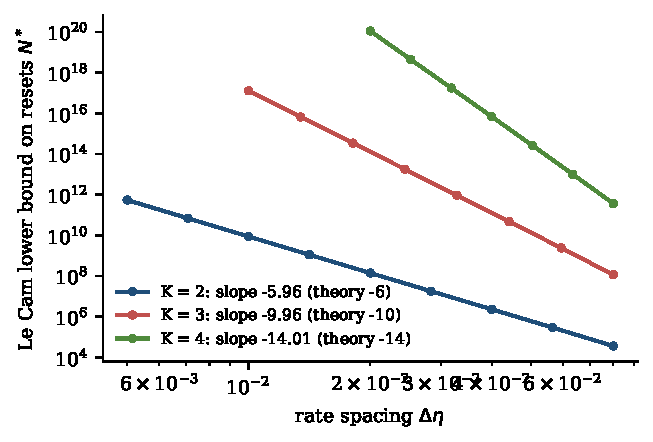
\includegraphics[width=0.62\textwidth]{figs/fig_kcohort.pdf}
\caption{Two-point lower bound on the number of reset experiments needed to separate $K$-cohort economies, as a function of the rate spacing.}\label{fig:kcohort}
\end{figure}

\begin{theorem}[Matching upper bound for every $K$]\label{prop:esprit}
Fix $K\ge2$, a compact set $\mathcal S\subset\{s\in[-1,1]^K:s_1<\cdots<s_K\}$ of ordered rescaled rates with $\min_{i\ne j}|s_i-s_j|\ge\gamma>0$, and weights in $[\omega_{\min},\omega_{\max}]$ with $\omega_{\min}>0$. Consider the class of $K$-cohort economies with rates $r_c+\Delta\eta\,s$, $s\in\mathcal S$, and $N$ independent reset experiments whose responses carry Gaussian noise with variance $\sigma^2$. There are constants $c_0,C>0$ depending only on $(K,\mathcal S,\gamma,\omega_{\min},\omega_{\max},a,\kappa,r_c)$ such that, whenever $\epsilon_N\equiv\sigma N^{-1/2}(\Delta\eta)^{-(2K-1)}\le c_0/\sqrt{\log(2/\beta)}$, Prony's method applied to the first $2K$ estimated kernel values, with its output atoms listed in increasing order of rate, recovers the weights with
\[
\max_i|\hat w_i-w_i|\;\le\;C\sqrt{\log(2K/\beta)}\;\epsilon_N
\]
with probability at least $1-\beta$. Hence $N=C'\sigma^2(\Delta\eta)^{-(4K-2)}$ experiments suffice for any fixed accuracy and confidence, and together with Theorem~\ref{thm:kcohort} the minimax sample requirement is $N^*\asymp\sigma^2(\Delta\eta)^{-(4K-2)}$.
\end{theorem}

\begin{proof}
The kernel values $k_m=\sum_iw_ir_i^m$ are the power moments of the merged measure. The closed-loop recursion $h_t=ah_{t-1}+\kappa\sum_mk_mh_{t-1-m}$ (plus $\kappa$ at $t=0$) can be solved for $k_0,\ldots,k_{2K-1}$ from $h_0,\ldots,h_{2K}$ with $h_0=\kappa\ne0$; the map is smooth with Lipschitz constant independent of $\Delta\eta$, so the estimated kernel values have error $O_P(\sigma N^{-1/2})$. Centring at $r_c$ is a fixed triangular linear map, $\mu_m=\sum_{j\le m}\binom mj(-r_c)^{m-j}k_j$, and $\mu_m=(\Delta\eta)^m t_m$ with $t_m=\sum_iw_is_i^m$. The map $F:(s,\omega)\mapsto(t_0,\ldots,t_{2K-1})$ does not depend on $\Delta\eta$; its Jacobian is a confluent Vandermonde matrix with determinant $\prod_i\omega_i\prod_{i<j}(s_i-s_j)^4$, bounded away from zero on the compact class. By the quantitative inverse function theorem there are $\rho_0>0$ and $L<\infty$, uniform over the class, such that $F^{-1}$ exists and is $L$-Lipschitz on the ball of radius $\rho_0$ around every point of $F(\text{class})$. An error $e$ in $\mu_m$ is an error $e(\Delta\eta)^{-m}$ in $t_m$, largest at $m=2K-1$. The observed response errors are Gaussian; after nonlinear deconvolution the kernel errors need not be exactly Gaussian. On the compact family, a local Lipschitz bound for that smooth map and Gaussian concentration for the response coordinates give, for sufficiently large $N$, $\|\hat t-t\|_\infty\le C_1\sqrt{\log(2K/\beta)}\,\epsilon_N$ with probability at least $1-\beta$. When this is below $\rho_0$, $\hat t$ lies in the ball where $F^{-1}$ is $L$-Lipschitz. The moment map is invariant to relabelling the atoms, so it is injective only on ordered nodes; on the class of ordered, $\gamma$-separated nodes it is injective, and the inverse function theorem applies there. Prony's method computes the algebraic inverse of the moment map up to the order of the atoms, so, listing its output in increasing order of rate (which the error bound below keeps unambiguous once $C\sqrt{\log(2K/\beta)}\,\epsilon_N<\gamma/2$), its output is $F^{-1}(\hat t)$ and the stated bound follows with $C=LC_1$ and $c_0=\rho_0/C_1$. The matching statement requires the class to contain the Gauss and Gauss--Radau pair of Theorem~\ref{thm:kcohort} (ordered nodes with separation at least the smaller of their two minimum gaps, and weights within $[\omega_{\min},\omega_{\max}]$ after scaling to total weight $W$); for any such class the orders match, with constants that depend on the class.
\end{proof}

Table~\ref{tab:kupper} confirms the order numerically. For numerical stability the estimator works in centred and rescaled coordinates (the estimator is the same; only its floating-point evaluation changes). The argument parallels the stability analysis of super-resolution for clustered complex nodes \citep{batenkov2021}, here for real nodes, and it reproduces the ESPRIT slope of $-6.15$ reported for $K=2$ in the earlier version.

\begin{table}[t]\centering\small
\begin{threeparttable}
\caption{Sample requirement of Prony's method against the lower-bound order}\label{tab:kupper}
\begin{tabular}{lcccc}
\toprule
 & $K=2$ & $K=3$ & $K=4$ & $K=5$\\
\midrule
Lower-bound order $-(4K-2)$ & $-6$ & $-10$ & $-14$ & $-18$\\
Fitted slope of $N^*$ in $\Delta\eta$ (Prony) & $-5.94$ & $-10.00$ & $-13.93$ & $-18.34$\\
\bottomrule
\end{tabular}
\begin{tablenotes}\footnotesize\item Rates $0.7+\Delta\eta\,s$ with $s$ the $K$-point Gauss nodes, total weight 0.1, $\Delta\eta\in[0.03,0.2]$; $N^*$ is the number of experiments for a weight RMSE of 10\% of the smallest weight, from 400 simulated estimates per point. \end{tablenotes}
\end{threeparttable}
\end{table}

\subsection{Near-colliding rates: a uniform rate for the merged measure}\label{sec:uniform}

Theorem~\ref{prop:esprit} needs the rates to stay $\gamma$-separated and every weight to stay away from zero. Neither restriction can be dropped for weight recovery: two atoms of weights $w$ and $W-w$ at rates $r$ and $r+\Delta$ and two of weights $W-w$ and $w$ at the same rates have merged measures that converge to the same measure as $\Delta\to0$, so no estimator recovers the individual weights uniformly over near-colliding economies. What can be recovered uniformly is the merged measure itself, in the permutation-invariant Wasserstein distance.

\begin{theorem}[Uniform rate without separation]\label{thm:uniformw1}
Fix $K\ge1$, a memory bound $\bar r<1$ and $0<m_{\min}\le B$. Let $\mathcal M_K$ be the merged measures with at most $K$ atoms in $[0,\bar r]$ and total mass $k_0\in[m_{\min},B]$, with no separation condition and no lower bound on individual weights, and write $\bar M=M/k_0$ for the normalized memory distribution. From $N$ reset experiments as in Theorem~\ref{prop:esprit}, let $\hat M$ be any element of $\mathcal M_K$ whose first $2K$ kernel values are closest in the sup norm to the estimated ones. There is $C$ depending only on $(K,\bar r,a,\kappa,B)$ such that, with probability at least $1-\beta$,
\[
W_1(\hat{\bar M},\bar M)\;\le\;C\Bigl(\frac{\sigma\sqrt{\log(4K/\beta)}}{m_{\min}\sqrt N}\Bigr)^{1/(2K-1)}\qquad\text{uniformly over }\mathcal M_K .
\]
Hence $N=O(\sigma^2m_{\min}^{-2}\epsilon^{-(4K-2)})$ experiments give accuracy $\epsilon$, and with the Wasserstein statement of Theorem~\ref{thm:kcohort} the minimax rate for the merged memory distribution is $N^{-1/(4K-2)}$, uniformly over near-colliding economies.
\end{theorem}

\begin{proof}
As in the proof of Theorem~\ref{prop:esprit}, the kernel values $k_0,\ldots,k_{2K-1}$ are a Lipschitz function of the first $2K+1$ responses on the bounded set of responses the class produces, so a union bound gives $\max_{t<2K}|\bar k_t-k_t|\le e=C_1\sigma\sqrt{\log(4K/\beta)/N}$ with probability at least $1-\beta$. The class is compact and the moment map continuous, so a closest element $\hat M$ exists, and $\max_t|k_t(\hat M)-k_t(M)|\le2e$ by the triangle inequality. Since all atoms lie in $[0,1]$, $|k_t|\le k_0$, and the normalized moments $m_t=k_t/k_0$ satisfy $|m_t(\hat M)-m_t(M)|\le2e/k_0+(|\hat k_t|/\hat k_0)(2e/k_0)\le4e/m_{\min}$. The affine map $r\mapsto2r/\bar r-1$ carries both normalized measures to distributions on $[-1,1]$ with at most $K$ atoms, multiplies $W_1$ by $2/\bar r$ and the differences of moments of order below $2K$ by at most $(1+2/\bar r)^{2K-1}$. The moment comparison inequality for $K$-atomic distributions on $[-1,1]$ \citep{wu2020}, $W_1\le c_K\delta^{1/(2K-1)}$ when the first $2K-1$ moments differ by at most $\delta$, then gives the bound with $C=c_K(\bar r/2)(1+2/\bar r)(4C_1)^{1/(2K-1)}$.
\end{proof}

The theorem separates two questions that Theorem~\ref{prop:esprit} answers together. Which memory distribution do the participants have? That has the same polynomial cost whether or not their rates collide. Which participant has which weight? That becomes impossible as rates collide, at any sample size. A supervisor who needs the first can have it at the rate of Theorem~\ref{thm:kcohort}; one who needs the second has to be told the number of cohorts and a separation, or has to obtain tagged data (Section~\ref{sec:disclosure}).

\subsection{General memory: the minimax rate is logarithmic}\label{sec:general}

Exponential memory is a modelling choice. Suppose instead that the feedback kernel is completely monotone, $k_m=\int_{[0,\rho]}r^m\,d\mu(r)$ with $\rho<1$, where $\mu$ is any nonnegative measure of total mass $W$: a finite or infinite mixture of exponential memories with merged weight $W$. Write $\mathcal M(\rho,W)$ for this class, assume the closed loop is uniformly stable, $s\equiv a+\kappa W/(1-\rho)<1$, and measure accuracy by
\[
d(\mu,\mu')=\sup\Bigl\{\textstyle\int f\,d(\mu-\mu'):\ f\ \text{1-Lipschitz on }[0,\rho],\ f(0)=0\Bigr\},
\]
which equals the Wasserstein-1 distance between measures of equal mass and also compares estimates whose mass is not exactly $W$. Let $E_L(|x|)$ denote the error of the best uniform approximation of $|x|$ on $[-1,1]$ by polynomials of degree $L$, and let $c_*=\inf_{L\ge1}L\,E_L(|x|)$. \citet{bernstein1914} showed that $L\,E_L(|x|)$ converges to a positive constant ($0.2802$; \citealp{varga1985}), so $c_*>0$; numerically $c_*=1/4$, attained at $L=2$ (Table~\ref{tab:general}).

\begin{lemma}[Moment-matched cohort pairs]\label{lem:altpair}
For every $n\ge2$ there are two probability measures on $[0,\rho]$, each with exactly $n$ atoms, whose moments of orders $0,\ldots,2n-2$ coincide and whose Wasserstein-1 distance is at least $\rho\,E_{2n-2}(|x|)\ge c_*\rho/(2n-2)$.
\end{lemma}

The atoms are the points where the best approximation of $|r-\rho/2|$ by polynomials of degree $2n-2$ attains its maximal error with alternating signs, and the weights are those of the divided difference on these points, which annihilates every polynomial of degree $2n-2$ (Appendix~\ref{app:proofs}). Each measure is an $n$-cohort economy.

\begin{theorem}[Minimax rate for general memory]\label{thm:general}
Let $N$ independent reset experiments observe the impulse response with Gaussian noise of variance $\sigma^2$ per tap, and let $B(\rho)=(1+\sqrt2)(1+2/\rho)$ and $C_h=\kappa^2/(1-s)^2$.
\begin{enumerate}[label=(\roman*)]
\item \emph{Lower bound.} Let $\Lambda_N=\log(N/\sigma^2)+\log\bigl(2C_h^2W^2/((1-\rho)\rho)^2\bigr)$. Whenever $\Lambda_N\ge4\log(1/\rho)$, every estimator $\hat\mu$ satisfies
\[
\sup_{\mu\in\mathcal M(\rho,W)}P_\mu\Bigl(d(\hat\mu,\mu)\ge\frac{c_*\,\rho W\log(1/\rho)}{\Lambda_N}\Bigr)\;\ge\;\frac1{4e},
\]
and the bound already holds over $n$-cohort economies, for a finite $n$ that grows with $N$.
\item \emph{Upper bound.} With $a$ and $\kappa$ known, invert the averaged response into kernel values $\hat k_0,\ldots,\hat k_L$, with $L+1=\lfloor\log(N/\sigma^2)/(4\log B(\rho))\rfloor$, and let $\hat\mu$ be any measure on $[0,\rho]$ minimizing $\max_{j\le L}|\int r^jd\hat\mu-\hat k_j|$ (a linear program). For every $\beta\in(0,1)$ there is $N_0$ depending only on $(\rho,W,a,\kappa,\beta)$ such that for $N/\sigma^2\ge N_0$,
\[
\sup_{\mu\in\mathcal M(\rho,W)}P_\mu\Bigl(d(\hat\mu,\mu)>\frac{3\pi\rho W\log B(\rho)}{\log(N/\sigma^2)}\Bigr)\;\le\;\beta .
\]
\end{enumerate}
Hence the minimax accuracy is of exact order $1/\log(N/\sigma^2)$, and reaching accuracy $w$ requires and suffices $N/\sigma^2=\exp(\Theta(1/w))$.
\end{theorem}

\begin{proof}[Proof sketch]
(i) Put the measures of Lemma~\ref{lem:altpair}, scaled to mass $W$, into the model. Their difference annihilates polynomials of degree $2n-2$, so the generating function of the kernel difference is $\int(1-rz)^{-1}d(\mu_A-\mu_B)=z^{2n-1}\int r^{2n-1}(1-rz)^{-1}d(\mu_A-\mu_B)$; on $|z|=1$ it is at most $2W\rho^{2n-1}/(1-\rho)$, and Parseval bounds $\|k^A-k^B\|_2$ by the same quantity. The response difference is $H_AH_B$ times the shifted kernel difference, so $\|h^A-h^B\|_2\le C_h\|k^A-k^B\|_2$. Choosing the smallest $n$ for which the Kullback--Leibler divergence of the $N$-sample experiments is at most one, the Bretagnolle--Huber form of Le Cam's lemma gives the bound with half the Wasserstein separation of the lemma. (ii) For a 1-Lipschitz $f$ with $f(0)=0$, Jackson's theorem gives a polynomial $q$ of degree $L$ with $\sup|f-q|\le\pi\rho/(4(L+1))$, and expanding $q$ in Chebyshev polynomials of $2r/\rho-1$ bounds the sum of its monomial coefficients by $\rho B(\rho)^{L+1}$. Hence $d(\hat\mu,\mu)\le\pi\rho(W+\delta)/(2(L+1))+2\delta\rho B(\rho)^{L+1}$, where $\delta$ is the largest kernel error. The kernel is recovered from the response by a series reciprocal, $K(z)=(1-az-\kappa/H(z))/(\kappa z)$, whose error is at most $2((1+s)/\kappa)^2(L+2)$ times the largest response error, so $\delta=O_P(\sigma N^{-1/2}L\sqrt{\log L})$. The choice of $L$ makes $\delta B(\rho)^{L+1}=O_P((\sigma^2/N)^{1/4}L\sqrt{\log L})$, negligible against the first term. Full proofs are in Appendix~\ref{app:proofs}.
\end{proof}

Theorem~\ref{thm:general} replaces a polynomial barrier with a logarithmic one. With exponential memory and $K$ known cohorts, halving the error multiplies the required number of experiments by a constant; with general memory, halving the error squares it. The lower bound holds already for finite mixtures, so knowing that the memory is a finite mixture of exponentials does not help unless the number of cohorts and their spacing are also known. The constants of the two bounds differ, by a factor that grows as $\rho\to1$, so the dependence on how long memory lasts is not pinned down. The source of the gap is visible in the proof: as $\rho\to1$ the moment-matched pairs separate their kernels more slowly ($\rho^{2n-1}$ decays slowly), which weakens the lower bound through $\log(1/\rho)$, while the upper bound pays $\log B(\rho)$, which stays bounded away from zero, for the conditioning of polynomial approximation on $[0,\rho]$. Logarithmic rates of this kind are familiar from deconvolution with supersmooth errors \citep{fan1991} and from moment methods for mixing distributions \citep{kong2017,wu2020}; here they arise from the closed loop of a market.

Table~\ref{tab:general} checks the construction and the estimator. The pairs of Lemma~\ref{lem:altpair} have exactly $n$ atoms, agree in all moments below order $2n-1$ to $10^{-61}$, and remain at Wasserstein distance about $0.4/n$, while the distance between their kernels shrinks by a factor of about $0.2$ per atom at $\rho=0.9$. The linear-programming estimator applied to a continuous memory distribution has error times $\log(N/\sigma^2)$ between $0.18$ and $0.28$ for $N$ from $10^4$ to $10^{24}$: a $10^{20}$-fold increase in data halves the error. The exponential-memory model of the previous subsections, where the cost is polynomial in $1/\Delta\eta$, is therefore the optimistic case: relaxing the parametric form makes identification from prices much harder, not easier.

\begin{table}[t]\centering\small
\begin{threeparttable}
\caption{General memory: moment-matched cohort pairs and the moment estimator}\label{tab:general}
\setlength{\tabcolsep}{3.5pt}
\begin{tabular}{lcccccc}
\toprule
\multicolumn{7}{l}{\emph{A. Best approximation of $|x|$}}\\
$L$ & 2 & 4 & 6 & 10 & 20 & 30\\
$L\,E_L(|x|)$ & 0.2500 & 0.2705 & 0.2756 & 0.2785 & 0.2797 & 0.2800\\
\midrule
\multicolumn{7}{l}{\emph{B. Pairs of Lemma~\ref{lem:altpair}}}\\
Atoms per measure $n$ & 2 & 4 & 6 & 8 & 10 & 12\\
$W_1(\mu_A,\mu_B)$, $\rho=0.9$ & 0.2250 & 0.1037 & 0.0669 & 0.0494 & 0.0391 & 0.0324\\
$n\,W_1$, $\rho=0.9$ & 0.450 & 0.415 & 0.402 & 0.395 & 0.391 & 0.388\\
$\|k^A-k^B\|_2$, $\rho=0.9$ & $4.41\times10^{-2}$ & $1.03\times10^{-3}$ & $4.08\times10^{-5}$ & $1.96\times10^{-6}$ & $1.05\times10^{-7}$ & $5.95\times10^{-9}$\\
$\|k^A-k^B\|_2$, $\rho=0.99$ & $7.41\times10^{-2}$ & $5.84\times10^{-3}$ & $1.07\times10^{-3}$ & $2.76\times10^{-4}$ & $8.33\times10^{-5}$ & $2.76\times10^{-5}$\\
\midrule
\multicolumn{7}{l}{\emph{C. Linear-programming estimator, continuous memory distribution, $\rho=0.9$}}\\
$\log_{10}N$ & 4 & 8 & 12 & 16 & 20 & 24\\
Moments used $L$ & 2 & 3 & 5 & 6 & 7 & 8\\
Error $d(\hat\mu,\mu)$ & 0.00878 & 0.00759 & 0.00432 & 0.00445 & 0.00382 & 0.00399\\
Error $\times\log(N/\sigma^2)$ & 0.202 & 0.245 & 0.179 & 0.226 & 0.229 & 0.276\\
\bottomrule
\end{tabular}
\begin{tablenotes}\footnotesize\item A: Remez algorithm; the limit is Bernstein's constant $0.2802$. B: moments of orders $0,\ldots,2n-2$ agree to $10^{-61}$ (60-digit arithmetic); every $W_1$ exceeds $\rho E_{2n-2}(|x|)$. C: true merged measure Beta(2,3) on $[0,0.9]$ with mass $0.1$; kernel values observed with noise $\sigma N^{-1/2}$, $\sigma=10^{-3}$; $L$ from the rule in Theorem~\ref{thm:general}(ii); measure fitted on a 401-point grid; 20 replications. Kind: recomputed (\texttt{general\_minimax.py}).\end{tablenotes}
\end{threeparttable}
\end{table}

\subsection{Passive data}

\begin{theorem}[Passive identification: minimum phase]\label{thm:minphase}
In a stable economy with $0<a<1$, distinct $0<r_i<1$ and nonzero merged weights, the zeros of $H$ are the memory rates $r_i$ together with a structural zero at $z=0$, and $H$ is minimum phase. Degenerate anchor and zero-rate cases require the cancellations described in the merged-equivalence proof. With a single price innovation, the price spectrum identifies $H$ up to scale, hence the memory rates; with $\kappa$ and $a$ known, as in Theorem~\ref{thm:merged}, it identifies the merged measure.
\end{theorem}

The result holds for signed weights (mean-reverting cohorts): in 1,733 stable random economies with weights of both signs, the nonstructural zeros equalled the memory rates and lay inside the unit disk. With a second independent shock in the cohorts' memories, the Jacobian of the price spectrum with respect to six model parameters has full rank, with singular values from $34.51$ down to $0.0698$. Passive noise helps identification rather than hindering it.

\begin{theorem}[Passive cost]\label{prop:passive}
Suppose the price is observed passively as the stationary output $x_t=H_\theta(L)\xi_t$ of a single innovation with variance $\sigma^2>0$, for $\theta$ in a compact, uniformly Schur-stable family with rates in $[\eta_{\min},\eta_{\max}]\subset(0,1)$, and let $D(\theta_1\|\theta_0)$ be the Kullback--Leibler divergence rate per observation.
\begin{enumerate}[label=(\roman*)]
\item For a single cohort at $\bar\eta$ against the symmetric pair at $\bar\eta\pm\delta$ with the same total weight, $D=\Theta(\delta^4)$.
\item For the moment-matched two-cohort economies of Theorem~\ref{thm:twocohort}, $D=\Theta(\tau^2(\Delta\eta)^6)$.
\item For every $K\ge2$, for the $K$-cohort Gauss and Gauss--Radau economies of Theorem~\ref{thm:kcohort}, $D=\Theta((\Delta\eta)^{4K-2})$.
\end{enumerate}
Hence any test based on $T$ passive observations with worst-case error at most $\alpha<1/4$ needs $T=\Omega(\delta^{-4})$, $T=\Omega(\tau^{-2}(\Delta\eta)^{-6})$ and $T=\Omega((\Delta\eta)^{-(4K-2)})$ respectively, and the likelihood-ratio test attains these orders as $T\to\infty$: passive data cost the same polynomial order as active probing for every number of cohorts.
\end{theorem}

The proof (Appendix~\ref{app:proofs}) combines the Whittle form of the divergence rate with the resolvent identity $H_1-H_0=H_1H_0(G_1-G_0)$: the two spectra differ by the leading unmatched moment, of order $\delta^2$ for the pair and $\tau(\Delta\eta)^3$ for the moment-matched economies, and the divergence rate is the square of that difference. Numerically, the fitted slopes of the required sample length are $-4.21$ and $-5.93$, against the theoretical $-4$ and $-6$; for part (iii) the fitted slopes of the Whittle divergence rate in $\Delta\eta$ are $5.91$, $9.98$ and $14.05$ for $K=2,3,4$, against $6$, $10$ and $14$ (\texttt{hardening/p1\_checks.py}).

Passive surveillance is possible in principle but costs the same polynomial order as active probing. Proposition~\ref{prop:passive0} is the exact finite-sample version for the known pair.

\section{Robustness to nonlinear and adaptive trading rules}\label{sec:learners}

The theorems of Sections~\ref{sec:ident}--\ref{sec:mixtures} use the linear exponential-memory recursion~\eqref{eq:cohort}. Real desks cap positions, trade only beyond thresholds, adapt their gains and learn online. A small probe of size $A$ moves the state by $O(A)$, so any rule whose order is a twice-differentiable function of an exponential-memory state is linear to first order and differs from it by $O(A^2)$; the theorems should then hold for small probes and fail for large ones. We check this, and locate where it fails, in simulations of five stylized rules at $a=0.5$, $\kappa=0.8$, total weight $q=0.2$ and mean rate $\bar\eta=0.4$, over 240 periods after a pulse probe.

The rules are: (1) \emph{momentum with a position limit}, the cohort's order a smooth saturating ($\tanh$) function of its memory state $y_{i,t}$, normalized to unit slope at the operating point; (2) a \emph{threshold rule} that trades only when $|y_{i,t}|>\tau=0.05$, in two versions, an exact dead zone and one averaged over background state variation of standard deviation $0.04$; (3) an \emph{adaptive-gain rule} in the form of recursive least squares with forgetting factor $1-\eta_i$, whose gain falls when the regressor is large; (4) an \emph{online neural readout}, a linear readout of a fixed two-layer $\tanh$ feature map with eight hidden units, trained by regularized stochastic gradient steps of size $\eta_i$; and (5) a \emph{tabular value rule} that updates a 21-bin table at rate $\eta_i$, in two versions, kernel-smoothed across bins and a single-bin lookup. These are stylized: each is built so that its small-signal dynamics are an exponential filter with rate $\eta_i$, and they are not calibrated to any production system.

Two checks follow the theory. \emph{Test~A (merged measure):} one cohort with weight $q$ and position limit $1$ against two cohorts with weights $q/2$ at the same rate and limits $0.55$ and $1.65$, so the two economies have the same merged measure; the raw response gap $\|X^{(1)}(A)-X^{(2)}(A)\|_2$ should be $O(A^2)$ (slope $2$ in $\log A$) and the probe-normalised gap $\|X^{(1)}(A)-X^{(2)}(A)\|_2/A$ should be $O(A)$ (slope $1$ in $\log A$) over $A\in[0.002,0.064]$. \emph{Test~B ($\delta^{-4}$ law):} one cohort at $\bar\eta$ against the symmetric pair at $\bar\eta\pm\delta$, $\delta\in[0.015,0.12]$, at probe size $A=0.005$; the normalized response difference $\|\Delta h\|_2$ should scale as $\delta^2$ and the certified capital of Theorem~\ref{thm:spectral} as $\delta^{-4}$. The saturation threshold $A_{\rm sat}$ is the smallest probe at which $\|\Delta h\|_2$ at $\delta=0.05$ departs by more than 10\% from its small-probe value.

To check that these conclusions do not depend on hand-built rules, we pre-registered a second experiment (\texttt{P1\_\allowbreak trained\_\allowbreak learners.json}, SHA-256 \texttt{3e8bf30cbfb6\ldots}) in which online learners are trained from scratch inside the closed-loop market for $T_{\rm burn}=5{,}000$ periods of flow and noise innovations; their learned parameters are saved and reloaded into the probing simulator without rescaling. Four learning rules are used: (i) recursive least squares with forgetting factor $\lambda=0.995$, learning its return-forecast slope; (ii) a two-layer $\tanh$ network with eight hidden units whose readout is trained by regularized online stochastic gradient descent on trading profit; (iii) a scalar policy-gradient rule trained on trading profit; and (iv) a tabular Q-learner with 21 states and 21 actions, TD(0) Bellman backups ($\gamma=0.90$) and Boltzmann action choice. Each learner acts on an exponential-memory state $y_{i,t}$ with rate $\eta_i$: training sets its response gain and curvature, not its memory rate, so the experiment asks whether learned policies preserve the merged-measure and $\delta^{-4}$ predictions, not whether learning produces exponential memory. The specification fixed four predictions: (a) a single exponential fits each trained learner's small-probe impulse response with $R^2\ge0.90$; (b) two trained populations with the same merged measure differ by at most $1\%$ in relative $L_2$ response at $A=0.005$; (c) the certified capital to separate trained populations whose memory rates differ by $2\delta$ scales with log--log slope in $[-4.15,-3.85]$; and (d) we report where equivalence and the $\delta^{-4}$ law fail when learning continues during the probe. A first implementation of this experiment did not pass the trained parameters to the probing simulator; the results below come from the corrected implementation (\texttt{validate\_\allowbreak trained\_\allowbreak learners\_\allowbreak hardened.py}), which reloads the saved parameters.

\begin{table}[t]\centering\footnotesize
\begin{threeparttable}
\caption{Merged-measure equivalence and the $\delta^{-4}$ law under stylized nonlinear rules and closed-loop trained online learners}\label{tab:learners}
\setlength{\tabcolsep}{1.5pt}
\begin{tabular}{@{}lcccccc@{}}
\toprule
Rule & Test A raw & Test A norm.\ & Test B slope & Test B slope & Capital at & $A_{\rm sat}$ /\\
 & ($O(A^2)$) & ($O(A)$) & ($\|\Delta h\|_2$) & (capital) & $\delta=0.05$ & $R^2_{\rm exp}$\\
\midrule
\multicolumn{7}{@{}l@{}}{\emph{Panel A. Stylized nonlinear and adaptive rules (fixed operating point)}}\\
Linear benchmark & --- & --- & $2.007$ & $-4.001$ & $61.42$ & ---\\
1. Momentum ($\tanh$ limit) & $2.015$ & $1.015$ & $2.007$ & $-4.001$ & $61.47$ & $0.834$\\
2. Threshold rule, averaged & $2.043$ & $1.043$ & $2.007$ & $-4.001$ & $61.42$ & $0.049$\\
3. Adaptive gain (RLS) & $2.064$ & $1.064$ & $2.007$ & $-4.001$ & $61.46$ & $0.751$\\
4. Online neural readout & $2.011$ & $1.011$ & $2.007$ & $-4.001$ & $61.48$ & $0.751$\\
5. Tabular value, smoothed & $2.039$ & $1.039$ & $2.007$ & $-4.001$ & $61.44$ & $1.271$\\
\midrule
\multicolumn{7}{@{}p{0.94\textwidth}@{}}{\emph{Panel B. Learners trained in the closed loop, saved and reloaded (frozen during the probe; shared training stream)}}\\
6. Recursive least squares & $3.000$ & $2.000$ & $2.008$ & $-4.014$ & $54.58$ & $R^2=0.993$\\
7. Two-layer network (SGD) & $1.878$ & $0.878$ & $2.007$ & $-4.012$ & $65.19$ & $R^2=0.994$\\
8. Policy gradient on profit & $3.000$ & $2.000$ & $2.004$ & $-4.006$ & $58.05$ & $R^2=0.995$\\
9. Tabular Q-learner (TD(0)) & $2.108$ & $1.108$ & $1.994$ & $-3.973$ & $186{,}821$ & $R^2=1.000$\\
\midrule
\multicolumn{7}{@{}l@{}}{\emph{Panel C. Where the trained-learner results change (range over the four learners)}}\\
Independent training streams & \multicolumn{2}{c}{rel.\ gap $\le10^{-5}$} & $0.13$ to $0.92$ & $-1.75$ to $-0.38$ & --- & (c) fails\\
Learning during the probe & \multicolumn{2}{c}{rel.\ gap $\le1.1\times10^{-3}$} & $1.99$ to $2.01$ & $-4.02$ to $-3.98$ & --- & (c) holds\\
\midrule
\multicolumn{7}{@{}p{0.82\textwidth}@{}}{Exact dead zone ($\tau=0.05$): $\|\Delta h\|_2=0$ at $A=0.005$; the probe moves the state past $\tau$ only for $A>0.139$.}\\
\multicolumn{7}{@{}p{0.82\textwidth}@{}}{Single-bin value lookup: $\|\Delta h\|_2=0$ at $A=0.005$; the probe leaves the central bin only for $A>0.149$.}\\
\bottomrule
\end{tabular}
\begin{tablenotes}\footnotesize\item Panel A: deterministic simulations around the operating point; Test A reports the raw response-gap slope in $\log A$ ($O(A^2)$) and the probe-normalised gap slope $\|X^{(1)}(A)-X^{(2)}(A)\|_2/A$ ($O(A)$, plotted in Figure~\ref{fig:learners}). Panel B: learners trained for $5{,}000$ periods, parameters saved and reloaded without rescaling and frozen during the probe; the two compared populations are trained on the same innovation stream; relative equivalence gaps at $A=0.005$ are at most $10^{-5}$. A raw Test A slope above $2$ means the gap is of higher order than $A^2$. Panel C: the same learners trained on independent innovation streams (first row) or updated at learning rate $0.35$ during the probe (second row). Capital in par units, certified bound of Theorem~\ref{thm:spectral} ($61.42$ for the linear model); the Q-learner settles on a small response gain ($0.022$), so separating it costs far more capital. Kind: recomputed (Panel A: \texttt{recompute\_p1\_learners.py} $\to$ \texttt{R\_P1\_learners.json}; Panels B--C: \texttt{validate\_trained\_learners\_hardened.py} $\to$ \texttt{R\_P1\_trained\_learners\_hardened.json}).\end{tablenotes}
\end{threeparttable}
\end{table}

\begin{figure}[t]\centering
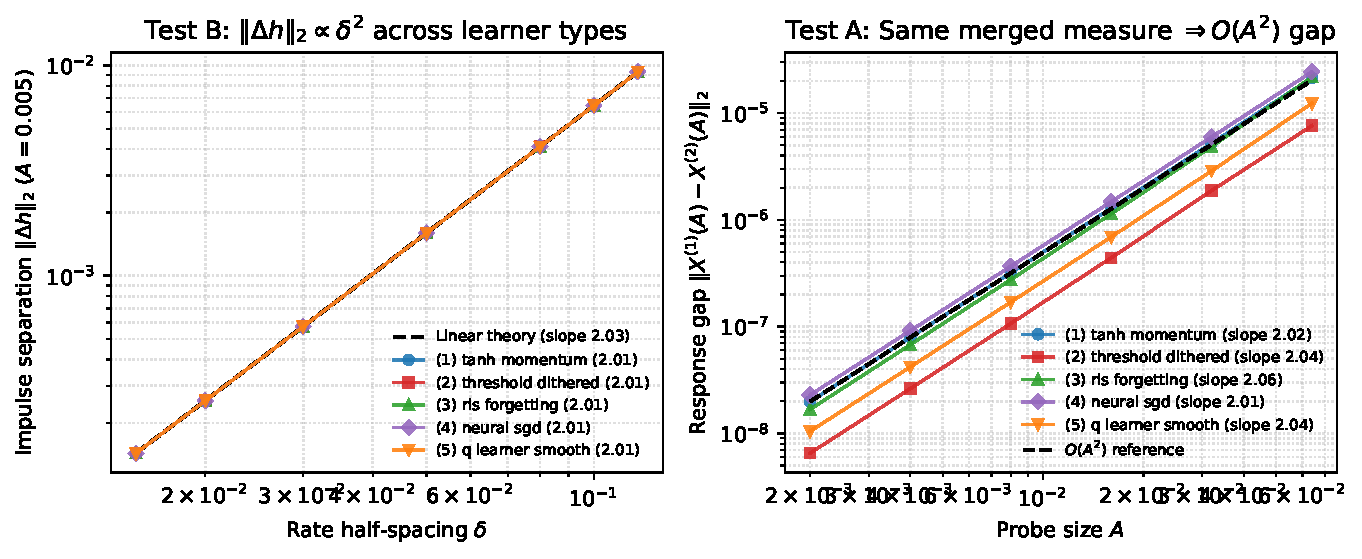
\includegraphics[width=0.92\textwidth]{figs/fig_learners.pdf}
\caption{Left: Test~B, probe-normalised response difference $\|\Delta h\|_2$ against the rate half-spacing $\delta$ at probe size $A=0.005$, five stylized rules and the linear benchmark. Right: Test~A, probe-normalised response gap $\|X^{(1)}(A)-X^{(2)}(A)\|_2/A$ between two economies with the same merged measure against the probe size $A$, with an $O(A)$ reference line (corresponding to an $O(A^2)$ raw gap).}\label{fig:learners}
\end{figure}

Table~\ref{tab:learners} and Figure~\ref{fig:learners} show both where the linear reduction holds and where it breaks down. In Panel~A, for small probes every smooth or dithered rule behaves like the linear model: economies with the same merged measure have raw response gap $O(A^2)$ (slopes $2.011$ to $2.064$) and probe-normalised gap $O(A)$ (slopes $1.011$ to $1.064$), while the response difference and certified capital scale as $\delta^2$ (slope $2.007$) and $\delta^{-4}$ (slope $-4.001$), with capital at $\delta=0.05$ within $0.1\%$ of the linear $61.42$. In Panel~B, predictions (a)--(c) pass for all four trained learners: a single exponential explains $R^2\ge0.993$ of each small-probe impulse response, populations with the same merged measure differ by at most $10^{-5}$ in relative response at $A=0.005$, and certified capital scales with slopes $-4.014$ to $-3.973$, inside the registered band. The level of capital differs across learners because training sets the response gain.

Panel~C shows where this changes. When the two populations are trained on independent innovation streams, prediction (c) fails: the capital slopes are $-1.75$, $-0.97$, $-1.62$ and $-0.38$. Independently trained populations end with learned gains that differ by sampling error of order $T_{\rm burn}^{-1/2}$, so they differ in merged weight as well as in memory rate, and a difference in weight is cheaper to detect than an $O(\delta^2)$ difference in rates. The $\delta^{-4}$ law therefore prices the separation of memory rates between populations whose feedback weights match; it is not a claim about telling apart any two trained populations. When learning continues during the probe at rate $0.35$, the law survives (slopes $-4.02$ to $-3.98$) and the merged-measure gap rises only to $1.1\times10^{-3}$, so the breakdown we anticipated under prediction (d) did not occur in this design.

The linear theory fails in two further places. First, saturation, adaptive gains and the neural readout leave the small-signal regime once probes exceed $A_{\rm sat}\in[0.751,1.271]$ par units, and the dithered threshold rule leaves it already at $A_{\rm sat}=0.049$, the threshold itself. Second, rules with hard discontinuities are different in kind: an exact dead zone ($\tau=0.05$) or a single-bin lookup does not respond at all to probes smaller than $0.139$ and $0.149$ par units ($\|\Delta h\|_2=0$), concealing those cohorts from small probes altogether. Neither smooth nonlinearity nor hard thresholds offers a cheaper route to separating memory rates than the linear benchmark; populations whose learned weights differ are told apart by their weights, not their rates.

\section{What disclosure buys}\label{sec:disclosure}

Because active probing is costly and passive data are slow, the natural policy question is what a supervisor gains from disclosure. We compare six observation contracts at $\delta=0.05$.
\begin{itemize}[itemsep=1pt]
\item $I_0$: public prices only.
\item $I_1$: prices and aggregated executed flow.
\item $I_2$: prices and one independent noisy report of dealer marked equity per reset ($\sigma_E=0.5$).
\item $I_3$: prices and exact audited equity (Proposition~\ref{prop:disclosure}), also with reports rounded to $0.01$.
\item $I_4$: algorithm update timestamps without the update values.
\item $I_5$: a supervisory audit registry with access to internal algorithm states.
\end{itemize}

\begin{table}[t]\centering\small
\begin{threeparttable}
\caption{Disclosure contracts at $\delta=0.05$ (pulse-design capital, par units)}\label{tab:contracts}
\begin{tabular}{llrrr}
\toprule
Contract & Channel & Pulses & Benchmark & Saving vs.\ $T=20$\\
\midrule
$I_0$: prices, $T=3$ & public prices & 271 & 4{,}305.25 & $-2{,}123.5\%$\\
$I_0^*$: prices, $T=20$ & full price path & 12 & 193.62 & 0.0\%\\
$I_1$: prices and signed flow & public flow & 12 & 193.62 & 0.0\%\\
$I_2$: noisy equity ($\sigma_E=0.5$) & statement & 12 & 193.62 & 0.0\%\\
$I_3$: exact equity, 5-unit lot & audited equity & 1 & 12.70 & 93.4\%\\
$I_3$: exact equity, 0.01 rounding & rounded report & 1 & 15.52 & 92.0\%\\
$I_4$: timestamps only & no likelihood & 12 & 193.62 & 0.0\%\\
$I_5$: audit registry & internal states & 0 & 0.00 & 100.0\%\\
\bottomrule
\end{tabular}
\begin{tablenotes}\footnotesize\item Closed-form values. Noisy equity adds information linearly in the number of resets, $\KL=N\Delta_E^2/(2\sigma_E^2)$, and saves only 1.5\% against the $T=3$ baseline. The equity difference is $\Delta E=\kappa^2q\delta^2V^2$; with reports rounded to $0.01$, a guaranteed change needs $V\ge5.59$.\end{tablenotes}
\end{threeparttable}
\end{table}

Table~\ref{tab:contracts} shows that disclosure is not one thing. Timestamps without update values carry no information about $\delta$ in this model. Noisy periodic statements barely help. Exact audited equity collapses the requirement to a single trade, limited only by lot sizes and report precision, and an audit registry removes the trading requirement altogether.

The cleanest form of useful disclosure is flow tagged by participant class.

\begin{proposition}[Tagged flow removes the barrier]\label{prop:tagged}
Let the price be driven by i.i.d.\ innovations of variance $\sigma_\xi^2$ in a positive, stable economy, with stationary autocovariances $\gamma_x(s)=\sum_\ell c_\ell\lambda_\ell^{|s|}$ ($c_\ell\ge0$, $0\le\lambda_\ell<1$ the closed-loop modes). Suppose the observer receives prices and each cohort's flow $\tilde u_{i,t}=u_{i,t}+\varepsilon_{i,t}$, $u_{i,t}=q_iy_{i,t}$, with i.i.d.\ measurement noise of variance $\sigma_f^2$ independent of prices. Then $\tilde u_{i,t}=r_i\tilde u_{i,t-1}+w_ix_t+e_{i,t}$ with $e_{i,t}=\varepsilon_{i,t}-r_i\varepsilon_{i,t-1}$, and the just-identified IV estimator of $\beta_i=(r_i,w_i)$ with instruments $Z_t=(x_{t-1},x_t)^\top$ satisfies $\sqrt T(\hat\beta_i-\beta_i)\to N(0,V_i)$,
\begin{equation}\label{eq:ivvar}
V_i=\Sigma_i^{-1}\Omega_i\Sigma_i^{-\top},\qquad \Sigma_i=\begin{pmatrix}w_iA_0&\gamma_x(1)\\ w_iA_1&\gamma_x(0)\end{pmatrix},\qquad \Omega_i=\sigma_f^2\bigl[(1+r_i^2)\Gamma_0-r_i(\Gamma_1+\Gamma_1^\top)\bigr],
\end{equation}
where $A_m=\sum_{s\ge0}r_i^s\gamma_x(s+m)$, $\Gamma_0=\begin{psmallmatrix}\gamma_x(0)&\gamma_x(1)\\ \gamma_x(1)&\gamma_x(0)\end{psmallmatrix}$ and $\Gamma_1=\E[Z_tZ_{t-1}^\top]$. The Jacobian determinant is
\begin{equation}\label{eq:ivdet}
\det\Sigma_i=w_i\sum_{\ell,m}c_\ell c_m\frac{1-\lambda_\ell\lambda_m}{1-r_i\lambda_m}\;>\;0 .
\end{equation}
$V_i$ depends only on cohort $i$'s own $(w_i,r_i)$, $\sigma_f^2$ and the price autocovariances, which are bounded and nondegenerate uniformly on a uniformly stable family whatever the rate spacing; so the merged weights are estimated at rate $T^{-1/2}$ with a constant that does not depend on $|r_i-r_j|$.
\end{proposition}

Each tagged flow follows $u_{i,t}=r_iu_{i,t-1}+w_ix_t$, a regression whose information about $w_i$ does not involve the other cohorts' rates; the closed form \eqref{eq:ivdet} matches the simulated Jacobian ($0.1330$ against $0.1322$ in a two-cohort economy with $4\times10^5$ periods; \texttt{hardening/p1\_checks.py}). In simulation ($T=5{,}000$, 60 replications) the root-mean-square error of the recovered weights is flat in $\Delta\eta$ (fitted slope $0.011$, error between $5.8\times10^{-4}$ and $6.6\times10^{-4}$). This is the formal content of a disclosure regime such as a consolidated audit trail: tagging flow by participant class turns a polynomial barrier into an ordinary estimation problem.

\subsection{How much disclosure is worth}\label{sec:discvalue}

Proposition~\ref{prop:tagged} says that tagging removes the barrier; the next result says by how much.

\begin{theorem}[Value of class-tagged disclosure]\label{thm:discvalue}
In the class of Theorem~\ref{prop:esprit}, let $N_p$ be the number of experiments needed with prices alone and $N_t$ the number needed with each class's flow observed with noise $\sigma_f$. To recover the weights to fixed accuracy, $N_p/N_t\asymp(\sigma/\sigma_f)^2(\Delta\eta)^{-(4K-2)}$; to resolve the rates to accuracy proportional to their spacing, $N_p/N_t\asymp(\sigma/\sigma_f)^2(\Delta\eta)^{-(4K-4)}$.
\end{theorem}

\begin{proof}
$N_p\asymp\sigma^2(\Delta\eta)^{-(4K-2)}$ by Theorems~\ref{thm:kcohort} and~\ref{prop:esprit}. With tagged flow each class is a single-exponential problem whose Fisher information for $(w_i,r_i)$ does not depend on the other classes, so $N_t\asymp\sigma_f^2$ for the weights and $N_t\asymp\sigma_f^2(\Delta\eta)^{-2}$ for rates resolved to a fraction of $\Delta\eta$.
\end{proof}

With the same noise and lags for both observers, the Cram\'er--Rao requirements give fitted slopes of $-6.08$ for prices and $-4.34$ for the ratio at $K=2$ (theory $-6$ and $-4$). Calibrated to the class memories estimated below, prices alone would need about 333 times as many days as the published class ratios to separate the top-trader and all-account memories in BTCUSDT (rates $0.9889$ and $0.9986$ per five minutes; about 6{,}000 days against 18), and about 19 times as many in ETHUSDT (rates $0.9793$ and $0.9972$). These rates come from day-demeaned regressions, which bias persistence down (Section~\ref{sec:disc_data}), so the factors are illustrative.

\subsection{Disclosure in dollars}\label{sec:disc_dollars}

Theorem~\ref{thm:discvalue} states the value of class-tagged disclosure in samples. Theorems~\ref{thm:spectral} and~\ref{thm:kcohort} let us translate that value into a flow of round-trip trading losses and set it beside the official operating budgets of the U.S.\ Consolidated Audit Trail (CAT). Two adjustments make the comparison exact and like-for-like:
\begin{enumerate}[label=(\roman*),itemsep=1pt]
\item \emph{Exact $K$-cohort moment-gap constant.} Rather than extrapolating from Cram\'er--Rao ratios, we evaluate the spectral round-trip trading loss bound of Theorem~\ref{thm:spectral},
\[
L_{\rm rt}^*(K,\Delta\eta)\;=\;\frac{4\sigma^2 z_{1-\alpha}^2}{\sup_\omega\bigl(|\Delta\hat H_{K,\Delta\eta}(e^{i\omega})|^2/g_0(\omega)\bigr)},
\]
directly for the $K$-point Gauss versus Gauss--Radau economies of Theorem~\ref{thm:kcohort} and Table~\ref{tab:radau}, whose moments below order $2K-1$ coincide and whose $(2K-1)$-th moment gap has the exact constant $\Delta_2=0.222222$, $\Delta_3=0.053333$, and $\Delta_4=0.013061$ at spacing $\Delta\eta$ (with $\Delta\eta=2\delta$ for the symmetric known pair).
\item \emph{Flow against flow.} A single probe loss $L_{\rm rt}^*$ is a one-time certification cost, whereas an audit trail is an ongoing annual expenditure. Because algorithm populations turn over and regulatory surveillance is periodic, we compare annual CAT operating costs against the annualised round-trip trading loss $52\times L_{\rm rt}^*$ under weekly certification renewal (matching the CFTC weekly reporting cycle of Section~\ref{sec:cot}). We benchmark against three primary official figures: the CAT LLC 2025 operating budget of $\$248.8$~million in the November 2024 filing (SEC Release No.\ 34-101901, Dec.\ 12, 2024, p.~4), revised to $\$228.3$~million in May 2025; the SEC's 2016 CAT NMS Plan Approval Order estimate of $\$2.4$~billion in initial industry build costs and $\$1.7$~billion per year in ongoing industry costs \citep[Release No.\ 34-79318, Nov.\ 15, 2016, 81 FR 84696 at 84801, p.~363]{sec2016}; and the SEC's Rule 613 proposing and adopting releases estimating $\$4.0$~billion initial and $\$2.1$~billion annual ongoing costs \citep[Release No.\ 34-62174, May 26, 2010, 75 FR 32556 at 32598, 32600, pp.~147, 153; Release No.\ 34-67457, July 18, 2012, 77 FR 45722 at 45790--45795, pp.~220--238]{sec2012}.
\end{enumerate}

\begin{table}[t]\centering\footnotesize
\begin{threeparttable}
\caption{Price-only round-trip probing loss per market and annualised weekly-renewal cost against official CAT budgets}\label{tab:cat_dollars}
\setlength{\tabcolsep}{1.5pt}
\begin{tabular}{@{}>{\scriptsize}l*{6}{>{\scriptsize}r}@{}}
\toprule
 & \multicolumn{2}{c}{\scriptsize Loss / probe (USDT)} & \multicolumn{2}{c}{\scriptsize Annual ($52\times$, USDT)} & \multicolumn{2}{c}{\scriptsize Mkts ($\$228.3$M / $\$1.7$B)}\\
Economy ($\Delta\eta$) & Roll & 1-sec & Roll & 1-sec & Roll & 1-sec\\
\midrule
$K=2$, known ($0.20$) & 6{,}200 & 149{,}901 & 322{,}400 & 7{,}794{,}852 & 708.1 / 5{,}273.0 & 29.29 / 218.09\\
$K=2$, known ($0.10$) & 99{,}192 & 2{,}398{,}422 & 5{,}157{,}984 & 124{,}717{,}944 & 44.3 / 329.6 & 1.83 / 13.63\\
$K=2$, known ($0.04$) & 3{,}874{,}696 & 93{,}688{,}369 & 201{,}484{,}192 & 4{,}871{,}795{,}188 & 1.1 / 8.4 & 0.05 / 0.35\\
\midrule
$K=2$, Radau ($0.20$) & 4{,}292 & 103{,}788 & 223{,}184 & 5{,}396{,}976 & 1{,}022.9 / 7{,}617.0 & 42.30 / 314.99\\
$K=2$, Radau ($0.10$) & 283{,}488 & 6{,}854{,}612 & 14{,}741{,}376 & 356{,}439{,}824 & 15.5 / 115.3 & 0.64 / 4.77\\
$K=3$, Radau ($0.20$) & 804{,}403 & 19{,}450{,}107 & 41{,}828{,}956 & 1{,}011{,}405{,}564 & 5.5 / 40.6 & 0.23 / 1.68\\
$K=3$, Radau ($0.10$) & 1{,}137{,}325{,}880 & 27{,}500{,}017{,}407 & 59{,}140{,}945{,}760 & 1{,}430{,}000{,}905{,}164 & 0.0 / 0.0 & 0.00 / 0.00\\
$K=4$, Radau ($0.20$) & 156{,}632{,}086 & 3{,}787{,}291{,}895 & 8{,}144{,}868{,}472 & 196{,}939{,}178{,}540 & 0.0 / 0.2 & 0.00 / 0.01\\
\bottomrule
\end{tabular}
\begin{tablenotes}\footnotesize\item Separation variable $\Delta\eta$ throughout ($\Delta\eta=2\delta$ for the symmetric known pair). Gauss--Radau rows use the exact $K$-cohort quadrature pair of Theorem~\ref{thm:kcohort} and Table~\ref{tab:radau} (moment gaps $\Delta_2=0.222222$, $\Delta_3=0.053333$, $\Delta_4=0.013061$ at $W=0.08$, $r_c=0.60$). Loss per probe is the spectral round-trip trading loss bound of Theorem~\ref{thm:spectral} at the median BTCUSDT Roll noise ($0.40$ USDT) and median one-second price-change standard deviation ($1.98$ USDT); annual loss multiplies by $52$ weekly renewals. The final columns divide the revised CAT LLC 2025 operating budget ($\$228.3$M; Nov.\ 2024 filing $\$248.8$M, SEC Release No.\ 34-101901, p.~4) and the SEC 2016 annual industry estimate ($\$1.7$B, Release No.\ 34-79318, p.~363) by the annual probing loss per market. Probing cost is a lower bound on the cost of learning from prices, not a social cost. Kind: recomputed (\texttt{recompute\_p1\_cat\_costs.py} $\to$ \texttt{R\_P1\_cat\_disclosure\_dollars.json}).\end{tablenotes}
\end{threeparttable}
\end{table}

Probing cost is a lower bound on the cost of learning from prices, not a social cost. Within that interpretation, Table~\ref{tab:cat_dollars} shows how rapidly the polynomial exponent $(\Delta\eta)^{-(4K-2)}$ and the shrinking Gauss--Radau moment-gap constant $\Delta_K$ turn the comparison in favour of disclosure. For a known pair at coarse separation $\Delta\eta=0.20$ ($\delta=0.10$), weekly price-only renewal costs $\$0.32$~million per market per year at Roll noise and $\$7.79$~million at one-second noise, so matching the $\$228.3$~million CAT LLC operating budget requires $708.1$ or $29.29$ markets. At $\Delta\eta=0.10$ ($\delta=0.05$) the unknown $K=2$ Gauss--Radau pair costs $\$14.74$~million (Roll) or $\$356.44$~million (one-second) per market per year, matching the CAT LLC budget in $15.5$ or $0.64$ markets and the SEC's $\$1.7$~billion industry figure in $115.3$ or $4.77$ markets. Once a supervisor must separate $K=3$ unknown cohorts at $\Delta\eta=0.20$, annual probing loss rises to $\$41.83$~million (Roll) and $\$1.01$~billion (one-second) per market ($5.5$ and $0.23$ markets at the CAT LLC budget; $40.6$ and $1.68$ markets at $\$1.7$~billion), and at $K=3, \Delta\eta=0.10$ or $K=4, \Delta\eta=0.20$ a single market's annual probing loss exceeds both the CAT LLC operating budget and the SEC's total annual industry estimate. The renewal frequency is an assumption: break-even market counts scale inversely with it, so monthly renewal multiplies every count in the last two columns by $4.3$ and renewal on each of 252 trading days divides them by $4.8$.

\subsection{Disclosure in real data}\label{sec:disc_data}

Binance publishes, every five minutes, long/short ratios for its top-trader group, by position and by account, and for all accounts. These are class-level positions, the closest public analogue to the tagged data of Proposition~\ref{prop:tagged}. We treat a class's reported net position as the observable counterpart of its cohort state: it obeys the same one-lag recursion class by class, so the block-diagonal information structure of Proposition~\ref{prop:tagged} carries over. The mapping is an assumption, because the reports are positions rather than flows and returns stand in for the unobserved deviation $x_t$. For each class $c$ we estimate $n_{c,t}=r_cn_{c,t-1}+w_c\,{\rm ret}_t$, with $n=(R-1)/(R+1)$ from the ratio $R$. The price-only alternative regresses signed five-minute taker flow on twelve lagged five-minute returns and fits two exponentials to the kernel; it estimates the memory rates without class information. Intervals come from a day bootstrap with 200 draws.

\begin{table}[t]\centering\small
\begin{threeparttable}
\caption{Memory rates with and without class-tagged data}\label{tab:disc}
\setlength{\tabcolsep}{3pt}
\begin{tabular}{lcccp{0.1\textwidth}p{0.08\textwidth}}
\toprule
Symbol & Days & Top position $\hat r$ [95\% CI] & All accounts $\hat r$ [95\% CI] & Width ratio & Classes differ\\
\midrule
BTCUSDT & 48 & 0.9889 [0.9842, 0.9935] & 0.9986 [0.9955, 1.0005] & 121.7 & yes\\
ETHUSDT & 48 & 0.9793 [0.9616, 0.9907] & 0.9972 [0.9934, 0.9997] & 55.6 & yes\\
CELRUSDT & 48 & 0.9884 [0.9830, 0.9922] & 0.9882 [0.9804, 0.9914] & 81.6 & no\\
CVXUSDT & 33 & 0.9822 [0.9732, 0.9908] & 0.9829 [0.9694, 0.9900] & 45.9 & no\\
\midrule
\multicolumn{6}{l}{\emph{Pre-registered test on fresh days, 30 USD-M perpetuals, 2025--2026}}\\
\multicolumn{3}{l}{(i) width ratio $>10$} & \multicolumn{3}{l}{30 of 30 (range 27.6--124.0)}\\
\multicolumn{3}{l}{(ii) price-only rate interval wider than 0.25} & \multicolumn{3}{l}{30 of 30 (range 0.65--0.99)}\\
\multicolumn{3}{l}{(iii) merged response $\sum_mk_m$ identified} & \multicolumn{3}{l}{5 of 30}\\
\multicolumn{3}{l}{Classes differ} & \multicolumn{3}{l}{11 of 30}\\
\bottomrule
\end{tabular}
\begin{tablenotes}\footnotesize\item Top panel: training days 2023--2024; width ratio is the mean price-only rate-interval width over the mean tagged width. The price-only intervals for both rates cover most of $[0,0.99]$. Bottom panel: specification registered before the fresh days were downloaded (SHA-256 \texttt{65acda361861\ldots}); a symbol passes if all three of the first rows hold, and the test required 80\% of symbols to pass. \end{tablenotes}
\end{threeparttable}
\end{table}

Table~\ref{tab:disc} gives three results. First, tagged class data restrict persistence rates that prices and flow leave essentially unrestricted: with the one-hour price-only kernel, the price-only intervals are 28 to 124 times wider in every one of 30 symbols on fresh days, and cover most of the admissible range. Part of this ratio is mechanical, because a series of positions identifies its own persistence directly while the price-only route must fit two exponentials to a weakly identified kernel. Restricting attention to the five symbols in which the price-only fit does identify the merged response (ACH, API3, OGN, ZEN and DASH) does not change the conclusion: the price-only rate intervals are still $0.64$ to $0.92$ wide and the ratios run from $27.6$ to $62.5$ (median $47.5$). We therefore read the ratios as a measure of how little prices reveal about class memory, not as a horse race between two estimators of equal standing. The ratios also overstate the gap for a second reason: the price-only kernel spans one hour (twelve five-minute lags), while the tagged half-lives are several hours, so the price-only fit cannot see memories of that length. An exploratory check on the 30 symbols and 105 days of the follow-up test refits the price-only kernel with 48 and 96 lags (four and eight hours) and compares both routes in one unit, the half-life. With 96 lags the price-only slow half-life (median 5.6 hours) reaches the tagged scale (median 4.2 hours). The tagged intervals remain narrower in all 30 symbols, but by a median factor of 7.5 in log half-life rather than 28 to 124, and the price-only interval still reaches a bound of the fit in 25 of 30. The horizon-matched comparison was then registered as a primary hypothesis of a test on 30 symbols never used in this project, before its data were downloaded, and passed: the tagged interval was narrower in 29 of 29 evaluable symbols (median factor 7.3, smallest 2.6), and the price-only interval reached a bound of the fit in 26. A registered secondary of the same test qualifies what the tagged estimate measures. Day-demeaned regressions bias persistence down; corrected by a split-panel jackknife, the median tagged rate is 1.0008 per five minutes, and the corrected interval lies below one in only 7 of 87 class fits. Within a day the class ratios are close to a random walk, so the half-lives of a few hours reported here are largely produced by removing each day's mean. The evidence therefore supports a narrower claim than identification of class memory: positioning data restrict a persistence parameter that prices cannot bound. Whether that persistence reflects learning memory or slow turnover of positions, which theory's tagged contract (class-tagged flow) would distinguish, is not established by these data. Second, the classes differ where theory says the information should be: in BTCUSDT and ETHUSDT the top-trader group's positioning has a half-life of about three to five hours against about one to two days for all accounts, while in thin symbols the classes are often indistinguishable. Third, the pre-registered test fails its 80\% criterion, on the part of the prediction that concerns what prices \emph{do} reveal: the merged response is significantly different from zero in only 5 of 30 symbols. Theorem~\ref{thm:minphase} says the merged measure is identified; on 42 days of thin-market data it is not estimated precisely. This is a failure of the prediction as registered, and we report it as one. A post hoc reading, not tested here, is that identification is an asymptotic statement and 42 days of passive thin-market data are far from that regime. Two follow-ups were registered before their data were downloaded, and each ran once. On 105 untouched days in the same 30 markets, price-only intervals were again at least ten times wider than class-tagged ones in all 30 symbols (median ratio 74.9 with the one-hour kernel), but the merged response was significantly different from zero in only 9 symbols, and pinning it down was at least ten times cheaper than separating the memory rates in only 10 of 30 (23 were required): that prediction failed. On 58 further days, the advantage of tagging grew with the sample in 22 of 29 symbols, the number required, but the tagged intervals shrank more slowly than the parametric rate (20 of 29 in the predicted range, 22 required), consistent with drift in class persistence over 21 months. Both results are reported in full in the companion thesis.

To test directly whether the memory rates identified by class-tagged positions improve out-of-sample return predictions after large order-flow shocks, we pre-registered a dedicated out-of-sample test (\texttt{P1\_disclosure\_oos.json}, SHA-256 \texttt{f0182ce50978\ldots}) before downloading the 22nd-of-month data for January 2025--September 2026 across 19 thin perpetuals ($6{,}137$ top-decile five-minute flow shocks on 2024 training days; $4{,}579$ shocks on untouched 2025--2026 test days). On the training sample we estimate each symbol's two memory rates $\hat r_1,\hat r_2$ either from the class-tagged positions or from the price-only two-exponential fit, construct the filtered memory states $y_{k,t}=\hat r_k y_{k,t-1}+(1-\hat r_k){\rm ret}_t$, and forecast the 30-minute post-shock cumulative return $R_{t+1\to t+6}$ out of sample relative to an AR(1) return-and-flow baseline. The primary hypothesis fails: on the untouched test shocks, the price-only memory states yield $\Delta R^2=-0.199$~percentage points relative to the baseline, the class-tagged memory states yield $\Delta R^2=-1.288$~points, and the tagged-minus-price-only difference is $\Delta R^2=-1.089$~points (95\% date-block bootstrap CI $[-2.605,+0.376]$, Clark--West $t=0.96$, $p=0.1684$). Likewise, adding the level and one-hour change of the top-trader and all-account positions to the hourly tail-risk controls of the companion paper leaves out-of-sample $R^2$ unchanged ($-0.19$~points, CI $[-0.99,0.83]$).

After this test failed, we registered a follow-up (\texttt{P1\_disclosure\_state\_oos.json}, SHA-256 \texttt{5136cc6b846d\ldots}) on untouched 2nd-and-9th-of-month data for January 2025--September 2026 across the same 19 thin perpetuals ($12{,}046$ top-decile five-minute flow shocks on 24 training dates in 2024; $9{,}875$ shocks on 42 test dates; test opened once). It asks the narrower question that Theorem~\ref{thm:merged} and Proposition~\ref{prop:tagged} answer directly: can prices and flow track the class states themselves? A two-exponential price-and-flow filter ($\alpha_{\rm fast}=0.50$, $\alpha_{\rm slow}=0.10$ on five-minute returns and signed flow, plus shock return, shock flow and symbol fixed effects) is compared with a filter that adds the current class states and their one-bar changes. Both registered primaries pass by a wide margin (Table~\ref{tab:disc_state_oos}): for the 30-minute-ahead divergence between top-trader and all-account positions, out-of-sample $R^2$ is $-4.8\%$ with prices and flow and $46.0\%$ with class data; for the top-trader state it is $4.4\%$ and $54.8\%$.

\begin{table}[!htbp]\centering\footnotesize
\begin{threeparttable}
\caption{Pre-registered out-of-sample cohort-state trajectory test on untouched 2nd-and-9th-of-month days (\texttt{P1\_disclosure\_state\_oos}), 2025--2026}\label{tab:disc_state_oos}
\setlength{\tabcolsep}{1.4pt}
\begin{tabular}{lccccc}
\toprule
30-min post-shock target (19 thin) & $R^2_{\rm pf}$ & $R^2_{\rm tag}$ & $\Delta R^2$ (pts) [95\% CI] & CW $t$ ($p$) & Res.\\
\midrule
Prim.\ 1: Divergence $d_{t+6}$ ($9{,}875$ shocks) & $-4.766$ & $45.962$ & $+50.728$ [$+45.291$, $+55.918$] & $21.27$ ($<10^{-16}$) & pass\\
Prim.\ 2: Top state $n_{{\rm top},t+6}$ ($9{,}875$ shocks) & $4.441$ & $54.845$ & $+50.404$ [$+47.226$, $+53.724$] & $21.85$ ($<10^{-16}$) & pass\\
Sec.: Divergence $d_{t+6}$, all ($210{,}144$ bars) & $-0.586$ & $37.053$ & $+37.639$ [$+36.232$, $+39.107$] & $72.75$ ($<10^{-16}$) & ---\\
Sec.: Top state $n_{{\rm top},t+6}$, all ($210{,}144$ bars) & $0.186$ & $46.779$ & $+46.593$ [$+45.555$, $+47.643$] & $80.44$ ($<10^{-16}$) & ---\\
\bottomrule
\end{tabular}
\begin{tablenotes}\footnotesize\item Out-of-sample $R^2$ in percent. Trained on 24 dates in 2024 ($12{,}046$ shocks, $120{,}384$ bars); evaluated once on 42 untouched test dates (2nd and 9th of each month, Jan 2025--Sep 2026); 2{,}000-draw date-block bootstrap 95\% CIs; Holm $p<10^{-16}$ across both primaries. Spec SHA-256 \texttt{5136cc6b846d\ldots} (\texttt{R\_P1\_disclosure\_state\_oos.json}).\end{tablenotes}
\end{threeparttable}
\end{table}

The gain is almost entirely persistence. In an exploratory decomposition on the same test shocks (\texttt{hardened\_empirical\_audits.py} $\to$ \texttt{R\_hardened\_empirical\_audits.json}), an AR(1) on the current level alone accounts for $100.5\%$ and $99.1\%$ of the improvement, and when the target is the 30-minute \emph{change} in positions the class data add $-0.26$ and $+1.41$ points. Because the class filter observes the series it forecasts, this is a weak test: it confirms that prices and flow cannot reconstruct where the classes are positioned, which Theorem~\ref{thm:merged} implies, but it does not show that class data reveal how their positions will move, and neither registered test finds that class data improve return forecasts.

\subsection{A second disclosure regime: the CFTC's trader-class reports}\label{sec:cot}

Binance publishes its class ratios voluntarily, for one venue. The U.S. Commodity Futures Trading Commission requires large traders in regulated futures markets to report their positions and publishes them weekly by class: leveraged funds, asset managers and dealers in financial futures, and managed money, producer/merchants and swap dealers in commodities. This is class-tagged disclosure mandated by law. We registered a test (SHA-256 \texttt{6f1d6f35ae88\ldots}) before downloading any data, in eight markets that span asset classes: CME Bitcoin and Ether, the E-mini S\&P 500, 10-year Treasury notes, the euro, the yen, WTI crude oil and Henry Hub natural gas, using every weekly report through October 2026 (282 to 1{,}039 weeks per market). For each class, $n_{c,t}=(\text{long}-\text{short})/\text{open interest}$ follows $n_{c,t}=\alpha_c+r_cn_{c,t-1}+w_c\,{\rm ret}_t$, the weekly version of the cohort recursion. The price-only alternative fits a two-exponential kernel to twelve weekly return lags. Intervals come from a 13-week moving-block bootstrap. The registered hypotheses were: (H1, primary) the fast class's memory rate is pinned to an interval narrower than $0.25$ while both price-only intervals are wider, in at least 75\% of markets; (H2) the fast class trend-follows, $w_c>0$, in at least 75\%; (H3) the fast class has the shorter memory in at least half.

\begin{table}[t]\centering\small
\begin{threeparttable}
\caption{Trader-class memory from the CFTC Commitments of Traders, eight regulated futures markets}\label{tab:cot}
\setlength{\tabcolsep}{3pt}\footnotesize
\begin{tabular}{lrccccr}
\toprule
Market & Weeks & Fast $\hat r$ [95\% CI] & Slow $\hat r$ & $\hat r_{\rm fast}-\hat r_{\rm slow}$ [95\% CI] & $\hat w_{\rm fast}$ & Ratio\\
\midrule
Bitcoin (CME) & 434 & 0.951 [0.928, 0.969] & 0.986 & $-0.035$ [$-0.062$, $-0.010$] & $-$ & 23.7\\
Ether (CME) & 282 & 0.890 [0.826, 0.932] & 0.960 & $-0.070$ [$-0.143$, $-0.011$] & $-$ & 9.1\\
E-mini S\&P 500 & 1{,}039 & 0.914 [0.884, 0.937] & 0.954 & $-0.040$ [$-0.071$, $-0.012$] & $-$ & 18.3\\
10-year T-note & 1{,}039 & 0.992 [0.985, 0.998] & 0.993 & $-0.000$ [$-0.006$, $+0.007$] & (0) & 71.4\\
Euro & 1{,}035 & 0.961 [0.947, 0.972] & 0.996 & $-0.034$ [$-0.051$, $-0.022$] & $+$ & 37.3\\
Yen & 1{,}035 & 0.955 [0.939, 0.968] & 0.984 & $-0.029$ [$-0.047$, $-0.013$] & $+$ & 34.0\\
WTI crude oil & 1{,}039 & 0.961 [0.946, 0.974] & 0.999 & $-0.037$ [$-0.053$, $-0.023$] & $+$ & 35.2\\
Natural gas & 1{,}039 & 0.981 [0.969, 0.990] & 0.980 & $+0.001$ [$-0.014$, $+0.017$] & $+$ & 44.0\\
\midrule
\multicolumn{7}{l}{\emph{Pre-registered hypotheses}: H1 (primary) 8 of 8, pass; H2 4 of 8, fail; H3 6 of 8, pass.}\\
\bottomrule
\end{tabular}
\begin{tablenotes}\footnotesize\item Fast class: leveraged funds (financial futures) or managed money (commodities); slow class: asset managers or producer/merchants. $\hat w_{\rm fast}$: sign of the response to returns, $+$ or $-$ when the 95\% interval excludes zero, (0) otherwise. Ratio: mean width of the two price-only rate intervals over the width of the fast-class interval; the price-only intervals span 0.95--0.96 of the admissible range $[0,0.99]$ in every market. Weekly returns from Binance spot (Bitcoin, Ether) and Yahoo Finance (others; the Treasury return is minus the change in the 10-year yield). Specification SHA-256 \texttt{6f1d6f35ae88\ldots}; test opened once. Kind: real data (Part 11).\end{tablenotes}
\end{threeparttable}
\end{table}

The primary hypothesis holds in all eight markets (Table~\ref{tab:cot}). The class reports pin each fast class's memory rate to an interval between $0.013$ and $0.106$ wide, while weekly prices leave both memory rates anywhere in the admissible range; the width ratios run from 9 to 71. The ratio partly reflects how little weekly returns reveal, which is the point of the theory rather than an artefact of it: with prices alone the memories are not located at all. The classes differ as the cohort model allows. Leveraged funds and managed money have the shorter memory in six of eight markets, with half-lives of 6 to 18 weeks against months to years for asset managers and producers; in Treasuries and natural gas the two memories are indistinguishable.

The trend-following hypothesis fails. The fast class buys after rises in the euro, the yen, crude oil and natural gas, but sells after rises in Bitcoin, Ether and the S\&P 500 futures. The first half matches the finding of \citet{moskowitz2012} that speculators' positions tend to go with past returns. We did not predict this. One candidate explanation is that leveraged-fund positions in financial futures are dominated by the short futures leg of cash--futures basis trades, which a single memory per class cannot represent. A post-hoc check is consistent with it but not decisive (Part 13, \texttt{R6}): weekly position changes of leveraged funds and asset managers are strongly negatively correlated in Bitcoin, Ether, the S\&P 500 and Treasuries ($-0.37$ to $-0.67$) but not in the euro or yen ($-0.04$ and $-0.05$), and holding the asset managers' change fixed removes the negative response in Bitcoin and halves it in Ether and the S\&P 500. Because class positions sum to zero across all reporting categories, some negative correlation is mechanical, so this is a signature, not a test. The failure sharpens rather than weakens the case for class tagging: class labels are not strategies, and a supervisor who wants to know how a class responds to prices needs its positions, which the price process does not reveal.

Together with Table~\ref{tab:disc}, the evidence now covers two disclosure regimes, one voluntary and one mandated by law, in crypto and in regulated equity-index, rate, currency and commodity futures. In both, class-tagged positions restrict persistence rates that prices leave unrestricted; whether that persistence is learning memory or slow turnover of positions, these data do not say.

\section{A spectral blind spot}
For any eigenvalues $0<\lambda_2<\lambda_1<1$, one-step price variance and sufficiently large stationary price variance, there is a family of two-state markets sharing all three quantities whose worst-case transient gain grows without bound (Supplemental Appendix, Theorem~\ref{thm:blind} and Figure~\ref{fig:blind}).

\section{Empirical feedback and its measurement}
Across a 96-date, eight-pair Binance spot panel (66.3M one-second bars), a 72-date BTCUSDT one-second panel, 30 USD-M perpetuals and two BTCUSDT spot zero-fee events, standard reduced-form feedback indices are dominated by EMA filtering mechanics ($1-\alpha=0.9355$) and clock alignment ($0.0081$ with look-ahead vs.\ $0.00037$ aligned); real feedback beyond the placebo is positive but small ($0.0045$), rises with market depth (Spearman $+0.70$), and does not move when zero fees multiply trading volume by $2.6$ to $4.9$ (Supplemental Appendix, Tables~\ref{tab:samples}--\ref{tab:fee2}).

\section{Implications for supervision and market design}\label{sec:policy}

\paragraph{What a supervisor can learn from public data.} Prices and anonymous flow reveal the merged measure $M$, the closed-loop impulse response and the reduced-form operator, and nothing finer. A supervisor who wants to know \emph{which} algorithms drive a feedback loop cannot get there from public data at reasonable cost when their memories are close. This is not a failure of econometric technique: Theorem~\ref{thm:twocohort} holds for every estimator, biased or not.

\paragraph{What probing costs.} At realistic observation noise, an exchange or a large desk could separate two well-separated memory rates for about $10^5$ USDT of capital. Probing is therefore feasible for coarse questions and infeasible for fine ones. Because capital grows as $\delta^{-4}$ and experiments as $(\Delta\eta)^{-(4K-2)}$, halving the separation multiplies the cost by 16 for a known pair and by $2^{4K-2}$ for $K$ unknown cohorts.

\paragraph{What disclosure buys.} Disclosure regimes differ sharply in value (Table~\ref{tab:contracts}). Timestamps without update values are worthless for this purpose. Noisy periodic statements are nearly worthless. Audited equity and, above all, flow tagged by participant class remove the barrier entirely (Proposition~\ref{prop:tagged}). This gives a quantitative argument for audit-trail regimes that record the participant class of each order, and a quantitative argument against relying on periodic statements for the same purpose. Calibrated to Binance's published class ratios, separating the memories of the top-trader group and of all accounts in BTCUSDT would take prices alone about 333 times as long (Theorem~\ref{thm:discvalue}). The class reports that the CFTC already requires have the same property in regulated markets (Table~\ref{tab:cot}), so the argument concerns the granularity and frequency of existing disclosure, not a new kind of reporting.

\paragraph{When audit trails already exist.} The US Consolidated Audit Trail (SEC Rule 613) gives the SEC and the self-regulatory organizations a record of every order in NMS stocks and listed options from origination to execution or cancellation, linked to an anonymized customer identifier and to the broker-dealer that handled it; since 2025 it no longer collects the names, addresses and years of birth of natural persons \citep{sec2012,sec2016,sec2024cat,sec2025}. Our results bear on such regimes in three ways. First, they price what the record is worth for the question of who drives a feedback loop: participant-level records remove a barrier that otherwise costs round-trip trading loss of order $\delta^{-4}$ and samples of order $(\Delta\eta)^{-(4K-4)}$ (Proposition~\ref{prop:tagged}, Theorem~\ref{thm:discvalue}); set against the CAT LLC 2025 operating budget ($\$248.8$~million in November 2024, revised to $\$228.3$~million in May 2025) and the SEC's 2016 annual industry estimate ($\$1.7$~billion), the annualised weekly-renewal probing loss that disclosure makes unnecessary is small for two well-separated classes and exceeds the entire CAT budget once $K\ge3$ at $\Delta\eta\le0.10$ or $K=4$ at $\Delta\eta=0.20$ (Section~\ref{sec:disc_dollars}, Table~\ref{tab:cat_dollars}). For this purpose a stable account identifier is what matters and names are not needed, which is a quantitative reason to keep the account linkage while removing personal data. Second, an audit trail records accounts, not decision rules. One account can run several algorithms and one algorithm can trade through several accounts, so an observer with account-level records who wants rule-level memories faces our problem within each account's flow, with fewer cohorts but the same exponent; MiFID II's algorithm identifier \citep{esma2016} is the closer analogue of the tagged flow in Proposition~\ref{prop:tagged}. Third, the audit trail does not reach the markets we study. Crypto perpetual futures are outside it, futures regulated by the CFTC have separate reporting, and its data are not available to exchanges, other participants or researchers. For these observers the price-only and coarse-disclosure contracts of this paper are the relevant ones.

\paragraph{What to monitor instead.} Because transient loss can be arbitrarily large at fixed eigenvalues and volatility (Theorem~\ref{thm:blind}), supervision that wants to control risk rather than identify participants should monitor quantities that bound transient loss directly: the summed absolute impulse response and operator confidence sets, both of which are identified from public data. These are cheap where identification is expensive (Remark~\ref{rem:riskneutral}); the companion paper shows that the summed response is certified at the parametric rate from controlled experiments, and only under a declared bound on memory length from a finite window \citep{niroula2026b}.

\paragraph{How to measure feedback.} Empirical feedback indices should (i) compare persistence with the mechanical value of the filter, (ii) align flow with the bar in which it is observed, (iii) control for order-splitting persistence or use instruments with a defended exclusion, and (iv) report placebo pipelines. Each of these changes the sign or the order of magnitude of published-style estimates in our data.

\section{Conclusion and an open problem}\label{sec:conclusion}

Prices reveal a merged summary of algorithmic feedback. Recovering the algorithms behind it costs executed quantity of order $\delta^{-2}$ and trading capital of order $\delta^{-4}$ for a known pair, with a certified constant of about 61 par units at the calibration, and a number of experiments of exact order $(\Delta\eta)^{-(4K-2)}$ for $K$ unknown cohorts, passively as well as actively; in simulations of stylized nonlinear rules and of online learners trained in the closed loop the same costs hold when the competing populations' feedback weights match, populations whose learned weights differ are told apart by those weights instead, and hard thresholds hide cohorts from small probes altogether. Without the exponential form, accuracy improves only as $1/\log N$, with matching lower and upper bounds. Class-tagged disclosure removes the barrier, and its value can be stated in samples and in dollars: a sample factor of order $(\Delta\eta)^{-(4K-4)}$, about 333 for the trader classes Binance already publishes in BTCUSDT, and an annualised weekly-renewal probing loss that matches the $\$228.3$~million CAT LLC operating budget across $15.5$ (Roll) or $0.64$ (one-second) markets for an unknown two-cohort Gauss--Radau pair at $\Delta\eta=0.10$ and exceeds it in a single market once $K\ge3$ at $\Delta\eta=0.10$; the CFTC's class reports restrict persistence rates that prices leave unrestricted in all eight regulated markets we examined, while a pre-registered out-of-sample test finds that class-tagged memory states do not improve 30-minute post-shock return forecasts ($\Delta R^2=-1.09$ points). At realistic noise the capital barrier for a moderate separation is about $10^5$ USDT. Measured feedback in crypto markets is real but small, rises with depth, does not move when fees change trading volume severalfold, and is easily confused with filtering and timing artefacts. Finally, eigenvalues and volatility cannot certify safety, because transient loss can be arbitrarily large at fixed spectrum and variance.

This leaves an open question for supervision: \emph{what can be measured and controlled without identifying the algorithms?} The impulse response $g_m=c^\top J^mb$, the operator $J$ and finite-sample confidence sets for it are identified from public data even when cohorts are not. The companion paper uses exactly this interface to build an identification-free pre-trade control.

\paragraph{Data and code availability.} All data are public: Binance archives (\url{https://data.binance.vision}), verified against published checksums. The pre-registered specification of the disclosure test, its SHA-256 hash and its test-set unlock counter are in the replication package. Every number in this paper is produced by a notebook cell or script that writes a result file (Appendix~\ref{app:repro}).

\paragraph{Use of AI tools.} The authors used Claude (Anthropic), an AI assistant, to write and debug analysis code, run checks of derivations and numerical results, and draft and edit text. Every number in the paper is produced by code the authors executed and archived in the replication package. The authors reviewed all content and take full responsibility for it.

\paragraph{Disclosures.} The authors declare no relevant financial interests.
\begin{thebibliography}{99}\setlength{\itemsep}{2pt}\small
\bibitem[Alfonsi et~al.(2016)]{alfonsi2016} Alfonsi, A., A. Schied, and F. Kl\"ock (2016). Multivariate transient price impact and matrix-valued positive definite functions. \emph{Mathematics of Operations Research} 41, 914--934.
\bibitem[Almgren and Chriss(2001)]{almgren2001} Almgren, R., and N. Chriss (2001). Optimal execution of portfolio transactions. \emph{Journal of Risk} 3, 5--39.
\bibitem[Batenkov et~al.(2021)]{batenkov2021} Batenkov, D., G. Goldman, and Y. Yomdin (2021). Super-resolution of near-colliding point sources. \emph{Information and Inference} 10, 515--572.
\bibitem[Bernstein(1914)]{bernstein1914} Bernstein, S. (1914). Sur la meilleure approximation de $|x|$ par des polyn\^omes de degr\'es donn\'es. \emph{Acta Mathematica} 37, 1--57.
\bibitem[Bessembinder et~al.(2006)]{bessembinder2006} Bessembinder, H., W. Maxwell, and K. Venkataraman (2006). Market transparency, liquidity externalities, and institutional trading costs in corporate bonds. \emph{Journal of Financial Economics} 82, 251--288.
\bibitem[Boehmer et~al.(2005)]{boehmer2005} Boehmer, E., G. Saar, and L. Yu (2005). Lifting the veil: An analysis of pre-trade transparency at the NYSE. \emph{Journal of Finance} 60, 783--815.
\bibitem[Bouchaud et~al.(2004)]{bouchaud2004} Bouchaud, J.-P., Y. Gefen, M. Potters, and M. Wyart (2004). Fluctuations and response in financial markets: The subtle nature of ``random'' price changes. \emph{Quantitative Finance} 4, 176--190.
\bibitem[Bouchaud et~al.(2018)]{bouchaud2018} Bouchaud, J.-P., J. Bonart, J. Donier, and M. Gould (2018). \emph{Trades, Quotes and Prices: Financial Markets Under the Microscope}. Cambridge University Press.
\bibitem[Brogaard et~al.(2014)]{brogaard2014} Brogaard, J., T. Hendershott, and R. Riordan (2014). High-frequency trading and price discovery. \emph{Review of Financial Studies} 27, 2267--2306.
\bibitem[Brunnermeier and Pedersen(2009)]{brunnermeier2009} Brunnermeier, M. K., and L. H. Pedersen (2009). Market liquidity and funding liquidity. \emph{Review of Financial Studies} 22, 2201--2238.
\bibitem[Cochrane and Orcutt(1949)]{cochrane1949} Cochrane, D., and G. H. Orcutt (1949). Application of least squares regression to relationships containing auto-correlated error terms. \emph{Journal of the American Statistical Association} 44, 32--61.
\bibitem[Colliard et~al.(2022)]{colliard2022} Colliard, J.-E., T. Foucault, and S. Lovo (2022). Algorithmic pricing and liquidity in securities markets. CEPR Discussion Paper 17606.
\bibitem[Dou et~al.(2025)]{dou2025} Dou, W.~W., I. Goldstein, and Y. Ji (2025). AI-powered trading, algorithmic collusion, and price efficiency. NBER Working Paper 34054.
\bibitem[ESMA(2016)]{esma2016} European Securities and Markets Authority (2016). Guidelines on transaction reporting, order record keeping and clock synchronisation under MiFID II. ESMA/2016/1452.
\bibitem[Fan(1991)]{fan1991} Fan, J. (1991). On the optimal rates of convergence for nonparametric deconvolution problems. \emph{Annals of Statistics} 19, 1257--1272.
\bibitem[Gatheral(2010)]{gatheral2010} Gatheral, J. (2010). No-dynamic-arbitrage and market impact. \emph{Quantitative Finance} 10, 749--759.
\bibitem[Glosten and Milgrom(1985)]{glosten1985} Glosten, L. R., and P. R. Milgrom (1985). Bid, ask and transaction prices in a specialist market with heterogeneously informed traders. \emph{Journal of Financial Economics} 14, 71--100.
\bibitem[Hasbrouck(1991)]{hasbrouck1991} Hasbrouck, J. (1991). Measuring the information content of stock trades. \emph{Journal of Finance} 46, 179--207.
\bibitem[Heinrich and Kahn(2018)]{heinrich2018} Heinrich, P., and J. Kahn (2018). Strong identifiability and optimal minimax rates for finite mixture estimation. \emph{Annals of Statistics} 46, 2844--2870.
\bibitem[Hendershott et~al.(2011)]{hendershott2011} Hendershott, T., C.~M. Jones, and A.~J. Menkveld (2011). Does algorithmic trading improve liquidity? \emph{Journal of Finance} 66, 1--33.
\bibitem[Hua and Sarkar(1990)]{hua1990} Hua, Y., and T. K. Sarkar (1990). Matrix pencil method for estimating parameters of exponentially damped/undamped sinusoids in noise. \emph{IEEE Transactions on Acoustics, Speech, and Signal Processing} 38, 814--824.
\bibitem[Kirilenko et~al.(2017)]{kirilenko2017} Kirilenko, A., A. S. Kyle, M. Samadi, and T. Tuzun (2017). The Flash Crash: High-frequency trading in an electronic market. \emph{Journal of Finance} 72, 967--998.
\bibitem[Kong and Valiant(2017)]{kong2017} Kong, W., and G. Valiant (2017). Spectrum estimation from samples. \emph{Annals of Statistics} 45, 2218--2247.
\bibitem[Kreiss(1962)]{kreiss1962} Kreiss, H.-O. (1962). \"Uber die Stabilit\"atsdefinition f\"ur Differenzengleichungen die partielle Differentialgleichungen approximieren. \emph{BIT Numerical Mathematics} 2, 153--181.
\bibitem[Kyle(1985)]{kyle1985} Kyle, A. S. (1985). Continuous auctions and insider trading. \emph{Econometrica} 53, 1315--1335.
\bibitem[Le Cam(1986)]{lecam1986} Le Cam, L. (1986). \emph{Asymptotic Methods in Statistical Decision Theory}. Springer.
\bibitem[Liu and Ammari(2022)]{liu2023} Liu, P., and H. Ammari (2022). Super-resolution of positive near-colliding point sources. arXiv preprint arXiv:2212.00536.
\bibitem[Makarov and Schoar(2020)]{makarov2020} Makarov, I., and A. Schoar (2020). Trading and arbitrage in cryptocurrency markets. \emph{Journal of Financial Economics} 135, 293--319.
\bibitem[Manole and Ho(2022)]{manole2022} Manole, T., and N. Ho (2022). Refined convergence rates for maximum likelihood estimation under finite mixture models. \emph{Proceedings of the 39th International Conference on Machine Learning}, PMLR 162.
\bibitem[Manski(2003)]{manski2003} Manski, C.~F. (2003). \emph{Partial Identification of Probability Distributions}. Springer, New York.
\bibitem[Niroula et~al.(2026)]{niroula2026b} Niroula, P., S. Alkhushayni, Y. Chen, M. Bhavsar, and P. Niroula (2026). From human markets to machine markets: Transient amplification, an exact depth condition, and a maximal pre-trade guard. Working paper, Minnesota State University, Mankato.
\bibitem[Moskowitz et~al.(2012)]{moskowitz2012} Moskowitz, T. J., Y. H. Ooi, and L. H. Pedersen (2012). Time series momentum. \emph{Journal of Financial Economics} 104, 228--250.
\bibitem[Obizhaeva and Wang(2013)]{obizhaeva2013} Obizhaeva, A. A., and J. Wang (2013). Optimal trading strategy and supply/demand dynamics. \emph{Journal of Financial Markets} 16, 1--32.
\bibitem[Pagano and R\"oell(1996)]{pagano1996} Pagano, M., and A. R\"oell (1996). Transparency and liquidity: A comparison of auction and dealer markets with informed trading. \emph{Journal of Finance} 51, 579--611.
\bibitem[Rivlin(1981)]{rivlin1981} Rivlin, T. J. (1981). \emph{An Introduction to the Approximation of Functions}. Dover.
\bibitem[Roll(1984)]{roll1984} Roll, R. (1984). A simple implicit measure of the effective bid-ask spread in an efficient market. \emph{Journal of Finance} 39, 1127--1139.
\bibitem[Roy and Kailath(1989)]{roy1989} Roy, R., and T. Kailath (1989). ESPRIT---estimation of signal parameters via rotational invariance techniques. \emph{IEEE Transactions on Acoustics, Speech, and Signal Processing} 37, 984--995.
\bibitem[SEC(2010)]{sec2010} U.S. Securities and Exchange Commission (2010). Risk management controls for brokers or dealers with market access. Release No.\ 34-63241.
\bibitem[SEC(2012)]{sec2012} U.S. Securities and Exchange Commission (2012). Consolidated Audit Trail; Final Rule (Release No.\ 34-67457, July 18, 2012, 77 FR 45722 at 45790--45795, pp.\ 220--238; proposing release No.\ 34-62174, May 26, 2010, 75 FR 32556 at 32598, 32600, pp.\ 147, 153).
\bibitem[SEC(2016)]{sec2016} U.S. Securities and Exchange Commission (2016). Joint Industry Plan; Order Approving the National Market System Plan Governing the Consolidated Audit Trail. Release No.\ 34-79318, November 15, 2016, 81 FR 84696 at 84801, p.\ 363.
\bibitem[SEC(2024)]{sec2024cat} U.S. Securities and Exchange Commission (2024). Notice of Filing of Proposed Rule Change Relating to the 2025 CAT Budget. Release No.\ 34-101901, December 12, 2024, p.\ 4 (revised May 2025).
\bibitem[SEC(2025)]{sec2025} U.S. Securities and Exchange Commission (2025). Order granting exemptive relief from certain requirements of the National Market System Plan governing the Consolidated Audit Trail. Release No.\ 34-102386, February 10, 2025.
\bibitem[Shleifer and Vishny(1992)]{shleifer1992} Shleifer, A., and R. W. Vishny (1992). Liquidation values and debt capacity: A market equilibrium approach. \emph{Journal of Finance} 47, 1343--1366.
\bibitem[Sornette et~al.(2023)]{sornette2023} Sornette, D., S. Lera, J. Lin, and K. Wu (2023). Non-normal interactions create socio-economic bubbles. \emph{Communications Physics} 6, 261.
\bibitem[Staiger and Stock(1997)]{staiger1997} Staiger, D., and J. H. Stock (1997). Instrumental variables regression with weak instruments. \emph{Econometrica} 65, 557--586.
\bibitem[Trefethen and Embree(2005)]{trefethen2005} Trefethen, L. N., and M. Embree (2005). \emph{Spectra and Pseudospectra: The Behavior of Nonnormal Matrices and Operators}. Princeton University Press.
\bibitem[Tsybakov(2009)]{tsybakov2009} Tsybakov, A. B. (2009). \emph{Introduction to Nonparametric Estimation}. Springer.
\bibitem[Varga and Carpenter(1985)]{varga1985} Varga, R. S., and A. J. Carpenter (1985). On the Bernstein conjecture in approximation theory. \emph{Constructive Approximation} 1, 333--348.
\bibitem[Wellman(2006)]{wellman2006} Wellman, M.~P. (2006). Methods for empirical game-theoretic analysis. In \emph{Proceedings of the 21st National Conference on Artificial Intelligence (AAAI-06)}, 1552--1555.
\bibitem[Whittle(1953)]{whittle1953} Whittle, P. (1953). Estimation and information in stationary time series. \emph{Arkiv f\"or Matematik} 2, 423--434.
\bibitem[Wu and Yang(2020)]{wu2020} Wu, Y., and P. Yang (2020). Optimal estimation of Gaussian mixtures via denoised method of moments. \emph{Annals of Statistics} 48, 1981--2007.
\end{thebibliography}

\appendix
\clearpage
\setcounter{page}{1}\renewcommand{\thepage}{S-\arabic{page}}
\setcounter{section}{0}\renewcommand{\thesection}{S.\arabic{section}}
\begin{center}{\Large Supplemental Appendix for ``Auditable Memory and Financial Identification Limits''}\end{center}
\label{app:suppstart}
\section{Map of results}
\begin{table}[t]\centering\small
\begin{threeparttable}
\caption{Map of results}\label{tab:map}
\begin{tabular}{p{0.34\textwidth}p{0.36\textwidth}p{0.18\textwidth}}
\toprule
Question & Answer & Where\\
\midrule
What do prices identify? & The merged rate--weight measure only & Thm~\ref{thm:merged}\\
Quantity to separate a known pair & $\Theta(\delta^{-2})$, exact error formula & Thm~\ref{thm:quantity}\\
Capital to separate a known pair & $\Theta(\delta^{-4})$, counterparty or own funds & Thm~\ref{thm:cap}, Lem.~\ref{thm:capital}\\
Constant at the calibration & $[61.41,64.48]$ par units; $\approx10^5$ USDT & Thms~\ref{thm:spectral}--\ref{thm:rh}, Table~\ref{tab:capital}\\
Does adaptivity help? & At most by a factor $\approx0.49$ in expected loss & Thm~\ref{thm:adaptive}\\
Unknown mixtures & $(\Delta\eta)^{-(4K-2)}$, tight for every $K$ & Thms~\ref{thm:kcohort}, \ref{prop:esprit}\\
General memory & Accuracy $\asymp1/\log N$, lower and upper bounds & Lem.~\ref{lem:altpair}, Thm~\ref{thm:general}\\
Passive data & Identifies $M$; same polynomial cost for every $K$ & Thms~\ref{thm:minphase}, \ref{prop:passive}, Prop.~\ref{prop:passive0}\\
Nonlinear and adaptive rules? & Settled online learners obey $\delta^{-4}$; fast adaptation or thresholds break it & Table~\ref{tab:learners}\\
What removes the barrier? & Tagged flow, audited equity & Props~\ref{prop:disclosure}, \ref{prop:tagged}\\
What is tagging worth? & Factor $(\Delta\eta)^{-(4K-4)}$; $\approx333\times$ for BTCUSDT (illustrative) & Thm~\ref{thm:discvalue}\\
Disclosure in dollars? & Annual probing loss exceeds CAT budget once $K\ge3$ or $\Delta\eta\le0.04$ & Table~\ref{tab:cat_dollars}\\
Do class data restrict class persistence? & Yes: 30 of 30, and 29 of 29 new markets (registered); whether it is memory is open & Table~\ref{tab:disc}\\
Can eigenvalues certify safety? & No & Thm~\ref{thm:blind}\\
What do feedback indices measure? & Mostly filtering and timing; small real feedback & Tables~\ref{tab:panel}, \ref{tab:feedback}\\
Does feedback track activity? & No: fees move volume 2.6--4.9$\times$, not $\hat Q$ & Table~\ref{tab:fee2}\\
\bottomrule
\end{tabular}
\end{threeparttable}
\end{table}
\section{Observation design and the tri-region partition}

An observer distinguishes two candidate mechanisms with rates $\theta_0$ and $\theta_1=\theta_0+\delta$ over $N$ periods, submitting probes $V=(V_1,\ldots,V_N)^\top$ that generate inventory $I_t=\sum_{s\le t}V_s$. Under contract $I_0$ (active probing, Gaussian observation noise) $p_t=(h_i*V)_t+\epsilon_t$, $\epsilon_t\sim N(0,\sigma^2)$, so
\begin{equation}\label{eq:klconv}
\KL(P_0^{\otimes N}\|P_1^{\otimes N})=\frac1{2\sigma^2}\sum_{t=1}^N\bigl((h_1*V)_t-(h_0*V)_t\bigr)^2 .
\end{equation}
The observer minimizes capital $C(N,V)=\sum_t(\lambda V_t^2+\phi|V_t|)+\max_t\mu p_0|I_t|$ subject to (i) separation $\KL\ge\tfrac12(z_\alpha+z_\beta)^2$, (ii) caps $|V_t|\le V_{\rm eff}$ and $|I_t|\le I_{\max}$, and (iii) a solvency budget $\max_t{\rm Loss}_t(V)\le B$. Here $V_{\rm eff}=\min(V_{\max},D_{\max}/\kappa)$ combines resting depth and a price-displacement limit.

\begin{proposition}[Tri-region partition and finite-session resolution floor]\label{prop:tri}
Under observation horizon $T$ per pulse, $(\delta,B)$ space splits into three regions.
\begin{enumerate}[label=(\roman*)]
\item \emph{Feasible single pulse.} For $\delta\ge\delta_{\min}(T)$ and $B\ge C^*(\delta)$ one pulse within capacity suffices. For a simple rate shift ($\eta_1=\eta_0+\delta$) the response difference is $\Theta(\delta)$ and $C^*=\Theta(\delta^{-2})$; for symmetric splitting the first-order variation cancels, the difference is $\Theta(\delta^2)$ and $C^*=\Theta(\delta^{-4})$.
\item \emph{Sequential bounded probing.} For $\delta<\delta_{\min}(T)$ the required quantity exceeds $V_{\rm eff}$. Capped pulses each supply divergence $V_{\rm eff}^2\|d_T\|^2/(2\sigma^2)$, so
\begin{equation}\label{eq:npulses}
N_{\rm pulses}(T,\delta)=\Bigl\lceil\frac{4\sigma^2z_\alpha^2}{V_{\rm eff}^2\|d_T\|_2^2}\Bigr\rceil .
\end{equation}
\item \emph{Infeasible with isolated pulses.} If the budget cannot finance sequential costs, peak inventory breaches $I_{\max}$, or a session deadline binds, the finite-session floor $\delta_{\min}(T_{\rm session})$ is the root of $V_{\rm eff}\|d_{T_{\rm cycle}}(\delta)\|_2=2\sigma z_\alpha/\sqrt{\lfloor T_{\rm session}/T_{\rm cycle}\rfloor}$, with small-$\delta$ approximation $\delta_{\min}=\Theta(T_{\rm session}^{-1/4})$.
\end{enumerate}
\end{proposition}

At the calibration $\kappa=0.8$, $q=0.2$, $\sigma=0.01$, $V_{\max}=50$, $D_{\max}=5$ ($V_{\rm eff}=6.25$), the single-tap floor is $\delta_{\min}(3)=\sqrt{2\sigma z_\alpha/(V_{\rm eff}\kappa^2q)}=0.2028$; extended observation lowers it to $0.1376$ ($T=4$), $0.0973$ ($T=10$), $0.0914$ ($T=20$) and $0.0905$ ($T=100$). At $\delta=0.05$ the simplified one-leg benchmark (cost $\tfrac12\kappa V_{\rm eff}^2+\phi P_*V_{\rm eff}=15.875$ per pulse plus initial margin $3.125$) needs 271 pulses and $4{,}305.25$ par units with $T=3$, 58 pulses and $923.88$ with $T=4$, but only 12 pulses and $193.63$ with $T=20$ and 11 pulses and $177.75$ with $T=100$; optimizing the pulse size (6.06 rather than 6.25) lowers the $T=20$ figure to $182.03$. Most of the saving comes from observing the transient response rather than a single tap (Figure~\ref{fig:phase}).

\begin{figure}[t]\centering
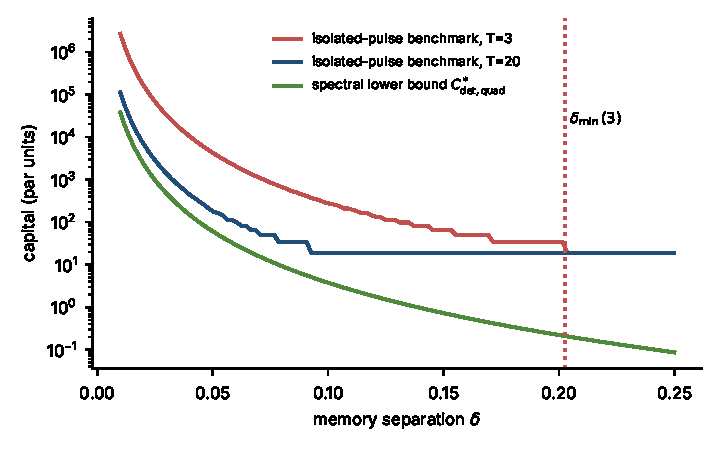
\includegraphics[width=0.62\textwidth]{figs/fig_phase.pdf}
\caption{Capital against separation: isolated-pulse benchmarks with three and twenty observations per pulse, and the spectral lower bound of Theorem~\ref{thm:spectral}. The dotted line is the single-tap resolution floor $\delta_{\min}(3)=0.2028$. Recomputed in this revision.}\label{fig:phase}
\end{figure} These are costs within an isolated-pulse design class, not minimum capital; the next subsection replaces the formula by a ledger.

\section{Robustness: heteroskedastic impact and probing protocols}

\begin{corollary}[Invariance under impact-induced heteroskedasticity]\label{cor:garch}
Suppose probing inflates innovation variance as $\sigma^2_{i,t}(v)=\sigma^2(1+\xi[(h_i*v)_t]^2)$ and slippage scales as $\kappa_{\rm eff}=\kappa(1+\xi_0|v_t|)$. For capacity-bounded probes, $\KL(P_0^v\|P_1^v)\le\frac{1+O(\xi^2V_{\rm eff}^2)}{2\sigma^2}\|(H_1-H_0)v\|_2^2=O(\|v\|_2^2\delta^4)$, and convex impact only raises dissipation. Required capital remains $\Theta(\delta^{-4})$.
\end{corollary}

Four probing protocols (unconstrained single pulse, repeated capped pulses, a sequential test with dynamic throttling, and a predetermined generalized-eigenvector trajectory) all show capital slopes near $-4$ in $\log\delta$: $-3.90$, $-3.84$, $-3.47$ and $-3.81$ over $\delta\in[0.03,0.12]$, where the sequential slope is flattened by the 1.7 pulses needed at $\delta=0.12$ (Appendix Table~\ref{tab:protocols}). At equal observation horizon, sequential stopping saves 14--49\% of capital relative to repeated capped pulses, but most of the apparent saving from the single-tap baseline comes from observing the transient response, not from adaptivity.

\section{A spectral blind spot\label{sec:blind}}

Even without identification, could a supervisor monitor risk through eigenvalues or volatility?

\begin{theorem}[Spectral blindness]\label{thm:blind}
For any eigenvalues $0<\lambda_2<\lambda_1<1$, one-step price variance $s_1>0$ and stationary price variance $V$ large enough, there is a family of two-state markets $J_\theta=\begin{psmallmatrix}\lambda_1&\theta\\0&\lambda_2\end{psmallmatrix}$ with shock covariance ${\rm diag}(s_1,s_2(\theta))$ such that all members share the eigenvalues, the one-step price variance and the stationary price variance, while the worst-case transient gain $\sup_k\|e_1^\top J_\theta^k\|$ grows without bound in $\theta$.
\end{theorem}

At $\lambda=(0.8,0.7)$, $s_1=1$ and $V=5$, the gain is $1.77$, $5.10$, $16.95$, $50.85$ and $169.50$ for $\theta=1,3,10,30,100$, with stationary variance $5.000$ in every case; the cumulative gain rises from $18.3$ to $1{,}667.7$. No monitor that depends only on eigenvalues and second moments of the price can be uniformly safe (Figure~\ref{fig:blind}).

\begin{figure}[t]\centering
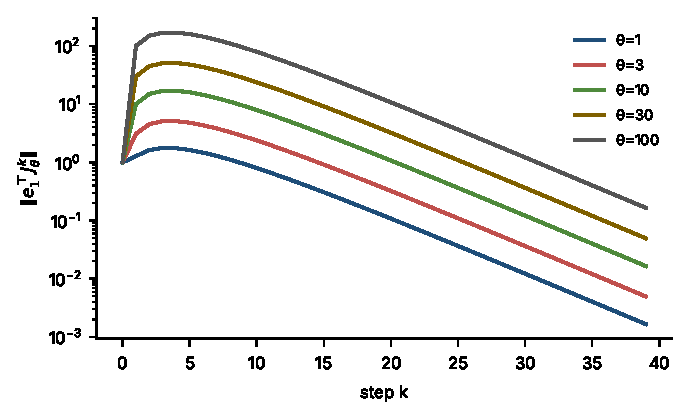
\includegraphics[width=0.6\textwidth]{figs/fig_blind.pdf}
\caption{Price-row transient gain of the spectral-blindness family $J_\theta$: eigenvalues $(0.8,0.7)$, one-step price variance 1 and stationary price variance 5 are the same for every $\theta$.}\label{fig:blind}
\end{figure}

Two clarifications prevent over-reading. First, the cohort economy of Section~\ref{sec:model} is itself non-normal, yet its price output does not amplify (Lemma~\ref{lem:cm}). Large weighted gains can be manufactured by output weights alone: with $C_w=(1,160)$, a price-and-memory functional peaks at $160.003$ at $t=0$, which is the static weight, not dynamic growth (Appendix~\ref{app:coordw}). Second, in a network of $M$ identical cohort economies coupled by symmetric nonnegative cross-impact, the coupled operator stays symmetric in the coordinates of Lemma~\ref{lem:cm}; with cross-impact $0.05$, the spectral radius rises from $0.822$ ($M=1$) to $0.973$ ($M=10$) while the Kreiss constant stays at one, as it must for a stable symmetric operator (\texttt{recompute\_oct20.py}). A stable normal contraction cannot exhibit Euclidean state-norm transient growth. This does not exclude scalar input-output overshoot relative to initial impact, which also depends on the input and output maps. The positive-cohort no-overshoot result is model-specific; the companion paper studies a depth-depletion mechanism.
\section{Empirical feedback and its measurement\label{sec:empirics}}

The theory says what prices can reveal. The empirical work has two roles, and neither is a test of the identification bounds themselves, which concern controlled experiments no outside researcher can run. First, Section~\ref{sec:disc_data} tests the theory's policy prediction directly: that class-tagged data pin down memories that prices leave unrestricted. Second, this section asks what the reduced-form feedback indices a supervisor would compute from public data actually measure, and how much of them is feedback rather than filtering, timing or trading activity.

\subsection{Estimand and filtering mechanics}

In theory $x_t=p_t-p^*_t$ is the deviation from an unobserved fundamental. Empirical work replaces $p^*_t$ by a trailing filter. Let $p_b$ be a log price proxy on uniform bars of length $\Delta$ and $m_b=(1-\alpha)m_{b-1}+\alpha p_b$ an exponential moving average with $\alpha=2/(W/\Delta+1)$. The empirical state is
\begin{equation}\label{eq:ema}
x^{\rm EMA}_b\equiv p_b-m_b=(1-\alpha)(p_b-m_{b-1})=\frac{1-\alpha}{1-(1-\alpha)L}\Delta p_b .
\end{equation}

Because $x^{\rm EMA}_{b+1}=(1-\alpha)(p_{b+1}-m_b)$, a martingale price gives
\begin{equation}\label{eq:mech}
\E[x^{\rm EMA}_{b+1}\mid\mathcal F_b]=(1-\alpha)x^{\rm EMA}_b :
\end{equation}
the filtered state is an AR(1) with mechanical persistence $a_0=1-\alpha$, which equals $29/31\approx0.9355$ for $W=300$ seconds and $\Delta=10$ seconds.

Let $f_t$ be signed flow. The empirical VAR(1)
\begin{equation}\label{eq:var}
\begin{pmatrix}x^{\rm EMA}_{t+1}\\ f_{t+1}\end{pmatrix}=\begin{pmatrix}J_{11}&J_{12}\\ J_{21}&J_{22}\end{pmatrix}\begin{pmatrix}x^{\rm EMA}_t\\ f_t\end{pmatrix}+e_{t+1}
\end{equation}
has reduced-form coefficients, not authenticated impact or learner parameters. When denominators are nonzero we use the scale-invariant indices
\begin{equation}\label{eq:QS}
\hat Q=\frac{\hat J_{12}\hat J_{21}}{1-\hat J_{22}},\qquad\hat S=\hat J_{11}+\hat Q,\qquad\hat L=\frac{\hat Q}{1-\hat J_{11}} .
\end{equation}
Equation~\eqref{eq:mech} implies that $\hat J_{11}$ must be compared with $1-\alpha$, not with zero: persistence that a naive reading attributes to feedback can be pure filtering.

\subsection{Data}

\begin{table}[t]\centering\small
\begin{threeparttable}
\caption{Samples}\label{tab:samples}
\begin{tabular}{p{0.32\textwidth}p{0.25\textwidth}p{0.18\textwidth}l}
\toprule
Sample & Coverage & Size & Source\\
\midrule
Binance spot panel, 8 pairs & 96 dates, 2021--2024 & 66.3M one-second bars & Binance archive\\
Binance spot fee-event windows, 8 pairs & $\pm20$ days around 2022-07-08 and 2023-03-22 & 640 pair-days & Binance archive\\
Binance USD-M perpetuals, 30 symbols & 90 dates, 2023--2026 & 2{,}565 symbol-days & Binance archive\\
Binance BTCUSDT one-second panel & 72 dates, 2021--2023 & 6.2M one-second bars & Binance archive\\
Binance BTCUSDT noise-calibration days & January 10--20, 2023 & 11 days & Binance archive\\
\bottomrule
\end{tabular}
\begin{tablenotes}\footnotesize\item Binance files are verified against the published SHA-256 checksums (every file used). Sampled dates are the 10th and 24th of each month.\end{tablenotes}
\end{threeparttable}
\end{table}

\subsection{Clock alignment dominates reduced-form feedback}

We estimate \eqref{eq:var} on ten-second bars built from one-second Binance klines across a 96-date, eight-pair spot panel (the 10th and 24th of each month, 2021--2024) under three constructions (Table~\ref{tab:panel}), and run the identical pipeline on a placebo random walk with each pair-day's volatility. Pairing the state with \emph{next-bar} flow (a look-ahead) gives $\hat Q=0.0081$; aligning flow with the bar in which it is observed lowers this by more than an order of magnitude, to $0.00037$; and replacing the EMA state by raw returns gives an interval that includes zero. Mean $\hat J_{11}$ under observed flow is $0.9203$, below the mechanical $0.9355$, and the placebo reproduces the mechanical value ($0.9351$) with $\hat Q$ indistinguishable from zero. 

\begin{table}[t]\centering\small
\begin{threeparttable}
\caption{Multi-year Binance spot panel: reduced-form indices under three timing constructions}\label{tab:panel}
\setlength{\tabcolsep}{2.5pt}
\renewcommand{\arraystretch}{1.1}
\begin{tabular}{p{0.2\textwidth}ccccc}
\toprule
Construction & $\hat Q$ & Date interval & $\hat S$ & Date interval & $\hat Q>0$\\
\midrule
Forward-paired flow (look-ahead) & 0.0081424 & [0.0072965, 0.0089882] & 0.92074 & [0.91665, 0.92482] & 87.4\%\\
Observed-flow EMA & 0.0003733 & [0.0002351, 0.0005116] & 0.92072 & [0.91640, 0.92504] & 62.4\%\\
Observed, 30 flow lags & 0.0002580 & [0.0001415, 0.0003745] & 0.91738 & [0.91167, 0.92308] & 59.1\%\\
Observed raw return & $-$0.0001555 & [$-$0.0003732, 0.0000622] & $-$0.04051 & [$-$0.05078, $-$0.03025] & 49.2\%\\
Placebo random walk & 0.0000016 & [$-$0.0000020, 0.0000052] & 0.93510 & [0.93485, 0.93534] & 51.0\%\\
\bottomrule
\end{tabular}
\begin{tablenotes}\footnotesize\item 768 study units (96 dates $\times$ 8 pairs), 6{,}634{,}752 ten-second transitions; equal-weight asset means within date, then date means with Student intervals. Mechanical persistence $29/31=0.93548$. \end{tablenotes}
\end{threeparttable}
\end{table}

\begin{table}[t]\centering\small
\begin{threeparttable}
\caption{Asset means under forward-paired and observed flow}\label{tab:assets}
\begin{tabular}{lcccc}
\toprule
Pair & Forward-paired $\hat Q$ & Observed $\hat Q$ & $\hat Q_{30}$ & Observed $\hat S$\\
\midrule
BTC/USDT & 0.0141870 & 0.0006073 & 0.0004891 & 0.93464\\
ETH/USDT & 0.0130885 & 0.0005675 & 0.0002549 & 0.93511\\
SOL/USDT & 0.0087763 & 0.0002129 & 0.0001100 & 0.91966\\
ADA/USDT & 0.0067465 & 0.0003928 & 0.0003546 & 0.91452\\
DOGE/USDT & 0.0058956 & 0.0002464 & 0.0001432 & 0.92496\\
BNB/USDT & 0.0057420 & 0.0004479 & 0.0002762 & 0.89533\\
XRP/USDT & 0.0057034 & 0.0002249 & 0.0001508 & 0.92362\\
LTC/USDT & 0.0049997 & 0.0002870 & 0.0002853 & 0.91792\\
\bottomrule
\end{tabular}
\begin{tablenotes}\footnotesize\item 96 dates per pair. $\hat Q_{30}$ controls 30 ten-second bars of lagged flow. Placebo $|\hat Q|\le1.1\times10^{-5}$ for every pair. \end{tablenotes}
\end{threeparttable}
\end{table}



\subsection{Feedback beyond filtering mechanics}

We re-estimate feedback on a separate sample and add a placebo. We use Binance BTCUSDT one-second klines on 72 sampled days in 2021--2023. The state $x_t$ is the log price deviation from its EMA (span 30 one-second bins), $f_t$ is next-second signed taker flow, and a VAR(1) gives $\hat Q$. Because the filter alone produces persistence, we run the identical pipeline on a placebo: a random walk with the same one-second volatility, independent of the real flow.

\begin{table}[t]\centering
\begin{threeparttable}
\caption{Feedback beyond filtering mechanics (Binance BTCUSDT, 72 days, 2021--2023)}\label{tab:feedback}
\begin{tabular}{lcc}
\toprule
 & Real prices & Placebo (independent random walk)\\
\midrule
Mean loop gain $\hat Q$ & 0.0045 & 0.0000009\\
95\% CI (day bootstrap) & [0.0034, 0.0056] & [$-$0.0000006, 0.0000023]\\
Mean price persistence $\hat J_{11}$ & 0.9364 & 0.9357\\
Mechanical value $1-2/31$ & \multicolumn{2}{c}{0.9355}\\
\bottomrule
\end{tabular}
\begin{tablenotes}\footnotesize\item Placebo 95\% band across days: $[-0.0000095,0.0000156]$. This construction pairs the state with next-second flow; it is not comparable in level with the observed-flow ten-second index of Table~\ref{tab:panel}.\end{tablenotes}
\end{threeparttable}
\end{table}

Table~\ref{tab:feedback} gives two findings. Feedback, in the sense of a loop gain the filter cannot produce, is detectable: the real $\hat Q$ lies far outside the placebo band. It is also small, and the price persistence that a naive reading would attribute to feedback is almost entirely mechanical ($0.9364$ against $0.9355$). Because this construction pairs the state with next-second flow, part of $\hat Q$ reflects the timing effect of Table~\ref{tab:panel}; the placebo shows only that the filter does not produce it.

\subsection{Order splitting and the estimation of feedback}

Persistent order flow makes lagged-flow regressions inconsistent. Suppose flow follows $q_t=\gamma y_t+u_t$ with memory $y_t=(1-\eta)y_{t-1}+\eta\Delta p_{t-1}$, order splitting $u_t=\rho u_{t-1}+\nu_t$, and $\Delta p_t=\kappa q_t+\lambda z_t+e_t$ with an observed exogenous price shock $z_t$. Lagged returns are correlated with $u_{t-1}$, so OLS of flow on returns is biased even when $\gamma=0$. Quasi-differencing ($q_t-\rho q_{t-1}=\gamma(y_t-\rho y_{t-1})+\nu_t$) or instruments that move $y$ through prices but are independent of $u$ ($z_{t-1},z_{t-2},z_{t-3}$) restore consistency. We compare estimators over 500 replications with $\eta=0.3$ and $\rho=0.8$ (Table~\ref{tab:iv}).

\begin{table}[t]\centering
\begin{threeparttable}
\caption{Feedback estimators under order splitting (simulation, 500 replications)}\label{tab:iv}
\begin{tabular}{lcccc}
\toprule
Estimator & Coverage at $\gamma=0.2$ & Rejection at $\gamma=0$ & Bias & RMSE\\
\midrule
OLS & 0.000 & 1.000 & 0.892 & 0.893\\
Cochrane--Orcutt, true $\rho$ & 0.944 & 0.054 & 0.001 & 0.039\\
Cochrane--Orcutt, estimated $\rho$ & 0.916 & 0.080 & 0.002 & 0.043\\
2SLS & 0.938 & 0.044 & $-$0.002 & 0.116\\
LIML & 0.938 & 0.044 & $-$0.003 & 0.117\\
\bottomrule
\end{tabular}
\begin{tablenotes}\footnotesize\item Newey--West standard errors (10 lags), $T=3{,}000$. Median first-stage $F=224$; a placebo instrument (future $z$) has $F=0.62$. Estimators outside 93--97\% coverage give invalid inference. \end{tablenotes}
\end{threeparttable}
\end{table}

OLS is badly biased. Cochrane--Orcutt with the true $\rho$, 2SLS and LIML have correct size and coverage; Cochrane--Orcutt with an estimated $\rho$ under-covers \citep{cochrane1949,staiger1997}. These are properties of estimators in a simulated market. On real data, a 2024 sub-panel of 192 spot units shows why the correction matters little at our bar length: with one VAR lag, the flow-equation residuals have essentially no first-order serial correlation (median $\hat\rho=-0.0002$), and Cochrane--Orcutt quasi-differencing moves the mean loop gain from $3.15\times10^{-4}$ to $3.21\times10^{-4}$ (Part 13, \texttt{R7}, post hoc). Order splitting shows up instead at longer lags, which the 30-lag control of Table~\ref{tab:assets} addresses. A real-data instrumental-variables estimate needs an instrument whose exclusion can be defended, which we do not claim to have; funding-settlement times, for example, may affect order flow directly.

Controlling for 30 ten-second bars of lagged flow lowers $\hat Q$ further (Table~\ref{tab:assets}, column $\hat Q_{30}$), consistent with persistent order splitting.

\subsection{Feedback across 30 perpetual markets}

The companion paper estimates the same loop gain on one-minute bars of 30 Binance USD-M perpetuals spread across the liquidity ranking (2023--2024 training days). Measured feedback rises with depth: its Spearman correlation with log depth within 1\% of the mid is $+0.70$ [$0.41$, $0.87$], from about $0.012$ in BTCUSDT and ETHUSDT to $0.0016$ on average in the thinnest third, and the placebo pipeline gives $\hat Q\approx0$ for every symbol. Feedback in this reduced-form sense is a feature of deep, algorithmically traded books.

\subsection{Two fee events}

Binance set spot trading fees on BTC pairs to zero on July 8, 2022 and reinstated them on March 22, 2023. Each event changes the cost of trading BTCUSDT while leaving the seven other pairs unchanged, and the second reverses the first. For every pair and every day within 20 days of each event we compute daily quote volume and the observed-flow $\hat Q$, and estimate $Y_{it}=\alpha_i+\gamma_t+\beta\,{\rm ZeroFee}_{it}+e_{it}$ with pair and date fixed effects and date-clustered errors, separately for each event and pooled (Table~\ref{tab:fee2}).

\begin{table}[t]\centering\small
\begin{threeparttable}
\caption{Zero fees on BTCUSDT: activity and measured feedback}\label{tab:fee2}
\begin{tabular}{lccc}
\toprule
 & Zero fees introduced & Zero fees removed & Pooled\\
 & (2022-07-08) & (2023-03-22) & \\
\midrule
Log quote volume, $\hat\beta$ & 0.945 (0.074) & 1.599 (0.080) & 1.272 (0.084)\\
Observed-flow $\hat Q$, $\hat\beta$ & 0.00058 (0.00032) & $-$0.00091 (0.00060) & $-$0.00016 (0.00036)\\
\quad $p$-value & 0.078 & 0.140 & 0.650\\
Pair-days & 320 & 320 & 640\\
\bottomrule
\end{tabular}
\begin{tablenotes}\footnotesize\item $\hat\beta$ is the effect of zero fees on BTCUSDT relative to seven control pairs; date-clustered standard errors in parentheses. For the second event ZeroFee equals one before March 22, 2023. \end{tablenotes}
\end{threeparttable}
\end{table}

The fee change moved activity enormously: zero fees multiplied BTCUSDT volume relative to the controls by $e^{0.945}\approx2.6$ when they began, and their removal divided it by $e^{1.599}\approx4.9$. Measured feedback did not follow. The two point estimates have opposite signs, neither is significant, and the pooled effect is $-0.00016$ with an interval of $[-0.00087,0.00055]$, against a sample mean of $0.00037$. A strong first stage with no second-stage response says that $\hat Q$ is not a by-product of trading activity, and the reversal design removes the main weakness of a single treated event. With one treated asset the interval remains wide, so this is evidence that $\hat Q$ does not scale with activity, not a proof of invariance.

\section{Proofs}\label{app:proofs}

\paragraph{Lemma~\ref{lem:micro}.} (i) For $v_{t+1}=v_t+\zeta_{t+1}$ and $r_t=v_t+\nu_t$, the steady-state prior variance $P$ solves $P=P\sigma_\nu^2/(P+\sigma_\nu^2)+\sigma_\zeta^2$, i.e.\ $P^2-\sigma_\zeta^2P-\sigma_\zeta^2\sigma_\nu^2=0$, whose positive root is $P=\bigl(\sigma_\zeta^2+\sqrt{\sigma_\zeta^4+4\sigma_\zeta^2\sigma_\nu^2}\bigr)/2$. The gain is $\eta=P/(P+\sigma_\nu^2)\in(0,1)$, which simplifies to \eqref{eq:kgain}, and the update $\hat v_{t+1}=\hat v_t+\eta(r_t-\hat v_t)$ has the stated form. (ii) $\nabla_\theta\tfrac12H(x_t-\theta)^2=-H(x_t-\theta)$, so $\theta_{t+1}=(1-\gamma)\theta_t+\alpha H(x_t-\theta_t)=(1-\eta)\theta_t+\eta qx_t$ with $\eta=\gamma+\alpha H$ and $q=\alpha H/\eta$.

\paragraph{Lemma~\ref{lem:cm}.} Omit zero-weight cohorts. For $a>0$ put $b_i=\kappa q_i$ and
\[
T={\rm diag}\bigl(\sqrt a,\sqrt{b_1/\eta_1},\ldots\bigr),\qquad u=\bigl(\sqrt a,\sqrt{b_1\eta_1},\ldots\bigr)^\top .
\]
The price-first transition becomes the symmetric matrix $J'=TJT^{-1}={\rm diag}(0,r_1,\ldots)+uu^\top$, the input transforms to $\kappa u$ and $J'e_x=\sqrt a\,u$, so $h_j=(\kappa/a)e_x^\top(J')^{j+1}e_x$. The spectral decomposition of $J'$ gives nonnegative weights summing to $h_0=\kappa$, and Schur stability puts the eigenvalues in $[0,1)$. The case $a=0$ follows by continuity. A nonnegative mixture of decaying geometric sequences is completely monotone. Since $J$ is nonnegative with row sums at most one, every price row of $J^t$ has $\ell_1$, hence $\ell_2$, norm at most one, attained at $t=0$.

\paragraph{Theorem~\ref{thm:merged}.} With zero initial states, $y_{i,t}=\sum_{s\le t}\eta_ir_i^{t-s}x_s$, so $\sum_iq_iy_{i,t}=\sum_{s\le t}k_{t-s}x_s$ and every response is determined by $(a,\kappa,k)$, hence by $M$. Conversely, equal responses for all probes imply equal $H$, hence equal $G$, and partial fractions of $G$ identify the distinct poles with nonzero residues $w_i$, i.e.\ $M$. After cancellation, $H=\kappa zD(z)/[(z-a)D(z)-\kappa N(z)]$ with $D=\prod(z-r_i)$ and $N(z)=\sum_iw_iz\prod_{j\ne i}(z-r_j)$, as in \eqref{eq:H}; at a retained $r_i$ the denominator equals $-\kappa N(r_i)=-\kappa w_ir_i\prod_{j\ne i}(r_i-r_j)\neq0$ (memory rates are positive because $\eta_i<1$), so no root of $D$ cancels. The remaining numerator factor $z$ cancels if and only if the denominator vanishes at $0$; since $N(0)=0$ the denominator there equals $-aD(0)$, which is nonzero for $a>0$ and zero for $a=0$. Hence the McMillan degree, which is the dimension of a minimal realization, is $1+|{\rm supp}(M)|$ for $a>0$ and $|{\rm supp}(M)|$ for $a=0$ (numerically, the rank of the Hankel matrix of $(h_j)_{j\ge1}$ is $K+1$ and $K$ respectively for $K=1,2,3$; \texttt{hardening/p1\_checks.py}). For (ii), direct algebra gives
\[
G_\delta(z)-G_0(z)=-\frac{qz(z-1)\delta^2}{(z-1+\bar\eta)\bigl((z-1+\bar\eta)^2-\delta^2\bigr)} .
\]
On $|z|=1$ each factor has modulus at least $\epsilon$. Uniform stability gives $M_H=\sup|H_\theta|<\infty$, and the identity $H_\delta-H_0=H_\delta H_0(G_\delta-G_0)$ gives an $\ell_2$ gain at most $K\delta^2$. The mean difference of a power-constrained probe has squared norm at most $K^2\delta^4PT$; the equal-noise KL is at most $K^2\delta^4PT/(2\sigma_\nu^2)$, and Pinsker's inequality with total variation at least $1-2\alpha$ gives \eqref{eq:Tpower}.

\paragraph{Theorem~\ref{thm:quantity}.} In either positive economy $J\ge0$ and $\|J\|_\infty\le1-\epsilon(1-S)<1$, so the response is nonnegative with $\max h=\kappa$ and $\sum h=\kappa/(1-S)$. From the display above, $|G_\delta-G_0|\le2q\delta^2/\epsilon^3$ on the circle; combined with the resolvent identity and positivity this gives $\|H_\delta-H_0\|_\infty\le K_*\delta^2$, and Parseval bounds $\|h^\delta-h^0\|_2$ by the same constant. Young's inequality gives $\|\mu_\delta-\mu_0\|_2\le K_*\delta^2\|v\|_1$, and Gaussian KL with Pinsker gives \eqref{eq:klV}. For (ii), the mean difference is a lower-triangular convolution matrix times $v$; each column is a shifted copy of a prefix of $d_T$, so $\|\mu_\delta-\mu_0\|_2\le V\|d_T\|_2$ with equality for a pulse at $t=0$. For two known equal-covariance Gaussian laws the minimax error is $\Phi(-\|\mu_\delta-\mu_0\|_2/(2\sigma))$, attained by the midpoint likelihood-ratio test. For (iii), the merged measures have equal mass and their first moments differ by $-q\delta^2$, which enters $h_2$ with factor $\kappa^2$ while $h_0,h_1$ coincide; a pulse $A$ separates the third-observation means by $A\kappa^2q\delta^2$. Part (iv) follows from the $\ell_2$ gain bound, and (v) from superposition and $\max_jh_j=\kappa$, which give $\sup_t|\lambda x_t|\le|\lambda|\kappa V$, attained by a single pulse.

\paragraph{Lemma~\ref{lem:toeplitz}.} After the uncontrolled update, the pre-probe displacement at step $j$ is $\sum_{i<j}h_{j-i}v_i$; average linear-book execution adds $\kappa v_j/2$. Summing signed execution costs gives $\tfrac12v^\top T_hv$. Each kernel $\lambda^{|i-j|}$ is a positive-definite AR(1) covariance for $0\le\lambda<1$, and a nonnegative mixture with positive total weight is positive definite. For a round trip the fundamental cash term cancels.

\paragraph{Theorem~\ref{thm:cap}.} Let $U_t=\sum_{j<t}v_j$. Positive responses give $0\le x_t\le\kappa U_t$ and $I_t=-U_t$. Summing cash and marking inventory, $B-E_t=U_tx_t-\sum_{j<t}v_jx^0_{j+1}-\tfrac\kappa2\sum_{j<t}v_j^2+cU_t$. Its quadratic part $v^\top A_tv$ has diagonal $h_{t-1-i}-\kappa/2$ and off-diagonal $\tfrac12(h_{t-1-i}+h_{t-1-j}-h_{j-i})$ for $i<j$; monotonicity of $h$ bounds every entry by $\kappa/2$. Hence $B-E_t\le\kappa U_t^2/2+cU_t\le\kappa V^2/2+cV$, while position value is at most $V(P_*+\kappa V)$; the stated inequality guarantees margin. A single pulse attains both adverse bounds at its first response, so no larger allowance is robust. Solving the quadratic gives \eqref{eq:VB}. The quantity requirement $V_B\gtrsim\delta^{-2}$ then forces $B\gtrsim\delta^{-4}$, and the pulse $A$ funded with $(\mu+\tfrac12)\kappa A^2+(c+\mu P_*)A$ attains it.

\paragraph{Proposition~\ref{prop:disclosure}.} The initial cash receipt is common to both alternatives and the dealer then holds $-A$. At time three $E_{3,r}=B+\kappa A^2/2-cA-A^2h_{r,2}$, so $E_{3,\delta}-E_{3,0}=A^2\kappa^2q\delta^2>0$.

\paragraph{Lemma~\ref{thm:capital}.} Marking residual inventory at $P_*$ gives $E_\infty=B-\tfrac12v^\top T_hv-c\sum|v_t|\ge0$. For each mode $\lambda\le r$ the Toeplitz kernel has spectral density $(1-\lambda^2)/(1-2\lambda\cos\omega+\lambda^2)\ge(1-r)/(1+r)$, so $v^\top T_hv\ge m\|v\|_2^2$ and $\|v\|_2^2\le2B/m$. The transfer bound gives mean-difference squared norm at most $K_*^2\delta^4\|v\|_2^2$, hence the KL bound; Pinsker gives \eqref{eq:Bmin}. For one pulse, cash becomes $B_A-A(P_*+\kappa A/2)-cA$ and inventory $A$; at later marks $E_t=\mu AP_*+A^2h_{t-1}$ and $\mu|I_t|P_t=\mu AP_*+\mu A^2h_{t-1}$, so margin holds for $\mu\le1$.

\paragraph{Proposition~\ref{prop:tri}.} Parts (i) and (ii) follow from \eqref{eq:klconv} with $\Delta h=\Theta(\delta)$ for a rate shift and $\Theta(\delta^2)$ for symmetric splitting, and from additivity of KL over independent pulse cycles. Part (iii) solves the session constraint for $\delta$; substituting $d_T(\delta)\approx\delta^2\tilde d_T$ gives the fourth-root approximation.

\paragraph{Theorems~\ref{thm:spectral} and~\ref{thm:adaptive}.} For a flat round trip, telescoping the cash account gives $L_i(v)=\tfrac12v^\top T_{h_i}v=\frac1{2\pi}\int g_i(\omega)|V(e^{i\omega})|^2d\omega$, with $g_i>0$ by Lemma~\ref{lem:cm}. Parseval gives $\|(H_1-H_0)v\|_2^2=\frac1{2\pi}\int|\Delta\hat H|^2|V|^2\le\sup_\omega(|\Delta\hat H|^2/g_i)L_i(v)$, and the Neyman--Pearson requirement $\|(H_1-H_0)v\|_2\ge2\sigma z_{1-\alpha}$ gives \eqref{eq:Cdet}. For adaptive policies, Doob's optional stopping theorem applied to the log-likelihood-ratio martingale and the data-processing inequality give $\E_0[\Lambda_\tau]\ge{\rm kl}(\alpha,1-\beta)$, while $\E_0[\Lambda_\tau]=\E_0\sum_t(\Delta\mu_t)^2/(2\sigma^2)\le\sup(|\Delta\hat H|^2/g_0)\E_0[L_0]/(2\sigma^2)$, which gives \eqref{eq:adaptive}.

\emph{Part (iv).} Let $G_\theta$ be the $T\times T$ lower-triangular Toeplitz section of $H_\theta/\kappa$, so the observation covariance is $\Sigma_\theta=\sigma_w^2G_\theta G_\theta^\top+\sigma_\nu^2I$. A finite section of a bounded analytic symbol has norm at most its supremum on the circle, so $\|G_\theta\|\le\sup_\omega|H_\theta|/\kappa\le\bar M$ because $|H_\theta(e^{i\omega})|\le\sum_jh_j=\kappa/(1-S)$. The inverse of a lower-triangular Toeplitz section is the section of the reciprocal series; $\kappa/H_\theta$ is analytic on and outside the unit circle because $H_\theta$ is minimum phase (Theorem~\ref{thm:minphase}), and Lemma~\ref{lem:cm} gives ${\rm Re}\,H_\theta(e^{i\omega})=\sum_\ell\omega_\ell(1-\lambda_\ell\cos\omega)/(1-2\lambda_\ell\cos\omega+\lambda_\ell^2)\ge\sum_\ell\omega_\ell/(1+\lambda_\ell)\ge\kappa/2$, so $\|G_\theta^{-1}\|\le2$ and $\Sigma_\theta\succeq\sigma_{\rm eff}^2I$ (the smallest singular value of $G_\theta$ is at least $0.522$ in 762 random positive economies and sections; \texttt{hardening/p1\_checks.py}). The Gaussian divergence splits into a mean and a covariance part. The mean part is $\tfrac12\Delta\mu^\top\Sigma_1^{-1}\Delta\mu\le\|(H_1-H_0)v\|_2^2/(2\sigma_{\rm eff}^2)$. For the covariance part, the eigenvalues $\lambda_k$ of $A=\Sigma_1^{-1/2}\Sigma_0\Sigma_1^{-1/2}$ are at least $c=\sigma_\nu^2/(\sigma_\nu^2+\sigma_w^2\bar M^2)$, and $\lambda-1-\log\lambda\le(\lambda-1)^2/\lambda$, so it is at most $\|A-I\|_F^2/(2c)\le\|\Sigma_0-\Sigma_1\|_F^2/(2c\,\sigma_{\rm eff}^4)$. Writing $\Sigma_0-\Sigma_1=\sigma_w^2(\Delta G\,G_0^\top+G_1\Delta G^\top)$ and $\|\Delta G\|_F^2\le T\|h^\delta-h^0\|_2^2/\kappa^2\le TK_*^2\delta^4/\kappa^2$ (proof of Theorem~\ref{thm:quantity}) gives a covariance part of at most $C_wT\delta^4$. The data-processing inequality turns errors $(\alpha,\beta)$ into $\KL\ge{\rm kl}(\alpha,1-\beta)$, and part (ii) bounds $\|(H_1-H_0)v\|_2^2$ by $\sup_\omega(|\Delta\hat H|^2/g_i)L_i(v)$, which gives \eqref{eq:Cnoise}.

\paragraph{Theorem~\ref{thm:rh}.} Write a feasible flat probe as $v=Eu$ and expand $u=\sum_jc_je_j$ in the $G_i$-orthonormal eigenbasis, so $L_i(v)=\sum_jc_j^2$ and the separation constraint reads $\sum_j\lambda_jc_j^2\ge c_{\rm req}$. Write the top-two component as $(c_{L-2},c_{L-1})=r(\cos\theta,\sin\theta)$ with $r\ge0$; replacing $\theta$ by $\theta+\pi$ flips $d$ and $s_\theta$ and leaves \eqref{eq:rhdefs} unchanged, so $\theta\in[0,\pi)$ suffices. Put $L_0(\theta)=c_{\rm req}/\lambda(\theta)$ and $D=L_i(v)-L_0(\theta)$. The constraint gives $r^2\lambda(\theta)\ge c_{\rm req}-\sum_{j\le L-3}\lambda_jc_j^2$, hence
\[
D=r^2+\sum_{j\le L-3}c_j^2-L_0(\theta)\;\ge\;\sum_{j\le L-3}\Bigl(1-\frac{\lambda_j}{\lambda(\theta)}\Bigr)c_j^2\;\ge\;\Bigl(1-\frac{\lambda_{L-3}}{\lambda(\theta)}\Bigr)\sum_{j\le L-3}c_j^2\;\ge0,
\]
and $r^2\ge L_0(\theta)-\frac{\lambda_{L-3}}{\lambda(\theta)}\sum_{j\le L-3}c_j^2\ge L_0(\theta)\bigl(1-\gamma(\theta)D\bigr)$. By H\"older's inequality with the sign vector $s_\theta$, $c_{\rm fee}\|Eu\|_1\ge c_{\rm fee}r\|Ed(\theta)\|_1+c_{\rm fee}\sum_{j\le L-3}c_j\,s_\theta^\top Ee_j$, and Cauchy--Schwarz with weights $1-\lambda_j/\lambda(\theta)$ bounds the second term below by $-\sqrt{D\,W_\perp(\theta)}$. Using $r\ge\sqrt{L_0(1-\gamma D)_+}\ge\sqrt{L_0}\,(1-\gamma D)_+$ and the fact that the fee is nonnegative, with $x=\sqrt D$,
\[
L_i(v)+c_{\rm fee}\|v\|_1\;\ge\;L_0(\theta)+x^2+\Bigl[F_{\rm dom}(\theta)(1-\gamma(\theta)x^2)_+-\sqrt{W_\perp(\theta)}\,x\Bigr]_+\;\ge\;L_0(\theta)+\Psi(\theta).
\]
Minimizing over the unknown $\theta$ gives \eqref{eq:rh}, and $\Psi\ge0$, $L_0(\theta)\ge c_{\rm req}/\lambda_{L-1}$ give the last inequality. On the piece $\gamma x^2\le1$ with $\gamma F_{\rm dom}<1$ the bracket is a convex quadratic in $x$ with minimum $F_{\rm dom}-W_\perp/(4(1-\gamma F_{\rm dom}))$, which gives the closed form.

\paragraph{Corollary~\ref{cor:garch}.} Since $\Delta h_t=O(\delta^2)$, the variance difference $\sigma^2_{1,t}-\sigma^2_{0,t}=\sigma^2\xi[(h_1+h_0)*v]_t[\Delta h*v]_t=O(\delta^2)$, and the variance term of the Gaussian KL, $\tfrac12\sum(x-1-\log x)$ with $x=\sigma^2_{0,t}/\sigma^2_{1,t}$, is quadratic in that difference. Convex impact only increases dissipation.

\paragraph{Proposition~\ref{prop:crb}.} Standard Cram\'er--Rao for a Gaussian mean model with Jacobian $J$. For $K=2$ the columns of $J$ for the two rates become collinear as $\Delta\eta\to0$; expanding to third order, the smallest singular value of $J$ is of order $(\Delta\eta)^3$, so $[F^{-1}]_{kk}=\Theta((\Delta\eta)^{-6})$.

\paragraph{Theorem~\ref{thm:twocohort}.} Expanding $M_m(\theta_1)-M_m(\theta_0)$ under \eqref{eq:pair} gives zero for $m\le2$ and $4\tau p_-p_+(\Delta\eta)^3$ for $m=3$. The map from moments to impulse responses is analytic with nonsingular derivative at the common limit, so $\|\Delta h\|_2=\Theta(\tau(\Delta\eta)^3)$. Le Cam's two-point lemma with $N$ independent Gaussian experiments gives \eqref{eq:lecam2}. For the permutation-invariant loss, the identity matching of $\theta_0$ and $\theta_1$ costs $2\tau+(p_+-p_-)\Delta\eta=2\tau(1+\Delta\eta/q)$ per atom and the swapped matching costs $\max(2p_+,2p_-)\Delta\eta=(1+2\tau/q)\Delta\eta$; when both are at least $2\tau$, any estimate within $\tau$ of one economy in $d_\infty$ is farther than $\tau$ from the other by the triangle inequality, and the two-point argument is unchanged. For (iii), the projection estimator of $M_3$ is unbiased with variance $\sigma_h^2/(N\|\nabla M_3h\|^2)$, and sub-Gaussian concentration gives the sample size; the Prony--Hankel determinant identity follows from $g_m=w_1\eta_1r_1^m+w_2\eta_2r_2^m$.

\paragraph{Theorem~\ref{thm:kcohort}.} Let $(s^A,\omega^A)$ and $(s^B,\omega^B)$ be the $K$-point Gauss and Gauss--Radau rules for the uniform weight on $[-1,1]$, normalized to unit mass. Both are positive and exact for polynomials of degree $2K-2$, and their moments of degree $2K-1$ differ by $g_K\neq0$. With $r=r_c+\Delta\eta\,s$ and weights $W\omega$, the raw moments $\sum w_ir_i^m$ are polynomials in $\Delta\eta$ that agree below degree $2K-1$, so the kernels differ by $O((\Delta\eta)^{2K-1})$ with nonzero leading coefficient; analyticity of the kernel-to-response map gives $\|h^A-h^B\|_2\asymp(\Delta\eta)^{2K-1}$, and Le Cam's lemma gives the bound. For the $W_1$ version, the two merged measures are the images of the fixed normalized rules under $s\mapsto r_c+\Delta\eta\,s$ scaled to mass $W$, so their distance is $W\Delta\eta$ times the distance $2c_K>0$ between the rules, and the same two-point argument applies with the metric loss.

\paragraph{Lemma~\ref{lem:altpair}.} Let $L=2n-2$ and let $p^*$ be the best uniform approximation of $|x|$ on $[-1,1]$ by polynomials of degree $L$, with error $E=E_L(|x|)$. By Chebyshev's equioscillation theorem \citep{rivlin1981} there are points $t_0<\cdots<t_{L+1}$ at which $|x|-p^*(x)$ equals $\pm E$ with alternating signs. The divided-difference weights $w_i=1/\prod_{j\ne i}(t_i-t_j)$ alternate in sign and satisfy $\sum_iw_ip(t_i)=0$ for every polynomial $p$ of degree at most $L$; multiplying by $-1$ if necessary, $w_i$ has the sign of $|t_i|-p^*(t_i)$ for every $i$. Exactly $n$ weights are positive and $n$ negative, and the positive and negative parts have equal mass because constants are annihilated. Normalizing each part to unit mass and mapping $x\mapsto\rho(x+1)/2$ gives $n$-atom probability measures $\pi_A$ (positive part) and $\pi_B$ (negative part) on $[0,\rho]$ with equal moments of orders $0,\ldots,L$. For the 1-Lipschitz function $f(r)=|r-\rho/2|=(\rho/2)|x|$,
\[
\int f\,d(\pi_A-\pi_B)=\frac\rho2\int\bigl(|x|-p^*(x)\bigr)\,d(\pi_A-\pi_B)=\frac\rho2(E+E)=\rho E ,
\]
because $p^*$ integrates to the same value under both measures, $|x|-p^*=E$ on the support of $\pi_A$ and $-E$ on that of $\pi_B$. By Kantorovich--Rubinstein duality $W_1(\pi_A,\pi_B)\ge\rho E\ge c_*\rho/L$.

\paragraph{Theorem~\ref{thm:general}.} Write $K(z)=\sum_mk_mz^m$, $D=1-az-\kappa zK$ and $H=\kappa/D$, which is the generating function of the recursion $h_t=ah_{t-1}+\kappa\sum_mk_mh_{t-1-m}$ with $h_0=\kappa$. Since $k_m\ge0$ and $\sum_mk_m=\int(1-r)^{-1}d\mu\le W/(1-\rho)$, the $\ell_1$ norm of $az+\kappa zK$ is at most $s<1$, so $\|H\|_1\le\kappa/(1-s)$ and $\|1/H\|_1=\|D\|_1/\kappa\le(1+s)/\kappa$.

(i) Let $\mu_A=W\pi_A$ and $\mu_B=W\pi_B$ with $\pi_A,\pi_B$ from Lemma~\ref{lem:altpair}; both lie in $\mathcal M(\rho,W)$. With $\nu=\mu_A-\mu_B$, $\sum_m(k^A_m-k^B_m)z^m=\int(1-rz)^{-1}d\nu(r)=z^{2n-1}\int r^{2n-1}(1-rz)^{-1}d\nu(r)$, because the first $2n-1$ terms of the geometric series integrate to zero. On $|z|=1$ the modulus is at most $2W\rho^{2n-1}/(1-\rho)$, so Parseval gives $\|k^A-k^B\|_2\le2W\rho^{2n-1}/(1-\rho)$. Next, $H_A-H_B=z(K_A-K_B)H_AH_B$, so by Young's inequality $\|h^A-h^B\|_2\le\|H_A\|_1\|H_B\|_1\|k^A-k^B\|_2\le C_h\|k^A-k^B\|_2$. The Kullback--Leibler divergence between the $N$-sample Gaussian experiments is $N\|h^A-h^B\|_2^2/(2\sigma^2)\le(N/\sigma^2)\,2C_h^2W^2\rho^{2(2n-1)}/(1-\rho)^2$, which is at most one as soon as $2(2n-1)\log(1/\rho)\ge\Lambda_N-2\log(1/\rho)$. Take $n$ the smallest integer with this property and $n\ge2$; then $2n-2<\Lambda_N/(2\log(1/\rho))$ when $\Lambda_N\ge4\log(1/\rho)$. Since $d$ is a norm on signed measures and $d(\mu_A,\mu_B)=W\,W_1(\pi_A,\pi_B)\ge Wc_*\rho/(2n-2)>2c_*\rho W\log(1/\rho)/\Lambda_N$, the Bretagnolle--Huber form of Le Cam's lemma \citep[Lemma 2.6 and Theorem 2.2]{tsybakov2009} gives $\max_{j\in\{A,B\}}P_j(d(\hat\mu,\mu_j)\ge c_*\rho W\log(1/\rho)/\Lambda_N)\ge\tfrac14e^{-1}$.

(ii) \emph{Approximation.} Let $f$ be 1-Lipschitz on $[0,\rho]$ with $f(0)=0$, so $|f|\le\rho$. The function $g(x)=f(\rho(x+1)/2)$ is $(\rho/2)$-Lipschitz on $[-1,1]$, and Jackson's theorem \citep{rivlin1981} gives a polynomial $p$ of degree $L$ with $\sup|g-p|\le(\pi/2)(\rho/2)/(L+1)\le\rho$, hence $\sup|p|\le2\rho$. Its Chebyshev coefficients satisfy $|b_j|\le2\sup|p|\le4\rho$. The polynomial $q(r)=p(2r/\rho-1)$ approximates $f$ with the same error, and its monomial coefficients satisfy $\sum_j|q_j|\le\sum_{j\le L}|b_j|\,\|T_j(2r/\rho-1)\|_{\rm coef}\le4\rho\sum_{j\le L}B(\rho)^j\le\rho B(\rho)^{L+1}$, where $\|\cdot\|_{\rm coef}$ is the sum of absolute monomial coefficients, $\|T_j\|_{\rm coef}\le(1+\sqrt2)^j$, substituting $y=\alpha r-1$ multiplies the coefficient sum of $y^i$ by at most $(1+\alpha)^i$, and $B(\rho)-1\ge4$. \emph{Moment comparison.} If $\max_{j\le L}|\int r^jd\hat\mu-k_j|\le2\delta$, then $\hat\mu$ has mass at most $W+2\delta$ and
\[
\int f\,d(\hat\mu-\mu)=\int(f-q)\,d(\hat\mu-\mu)+\sum_{j\le L}q_j\Bigl(\int r^jd\hat\mu-k_j\Bigr)\le\frac{\pi\rho(W+\delta)}{2(L+1)}+2\delta\rho B(\rho)^{L+1}.
\]
\emph{Kernel recovery.} From $\kappa zK=1-az-\kappa/H$, the kernel values $k_0,\ldots,k_L$ are the coefficients of $(1-az-\kappa/H)/(\kappa z)$, which depend on $h_0,\ldots,h_{L+1}$ only. Work in the algebra of power series modulo $z^{L+2}$ with the $\ell_1$ norm, which is submultiplicative. If the averaged response is $\hat H=H+E$ and $\|1/H\|_1\|E\|_1\le\tfrac12$, then $1/\hat H=(1/H)(1+E/H)^{-1}$ and $\|1/\hat H-1/H\|_1\le2\|1/H\|_1^2\|E\|_1$, so $\max_j|\hat k_j-k_j|\le\delta\equiv2((1+s)/\kappa)^2(L+2)\max_{t\le L+1}|E_t|$. Each $E_t$ is Gaussian with variance $\sigma^2/N$, so with probability at least $1-\beta$, $\max_t|E_t|\le\sigma\sqrt{2\log(2(L+2)/\beta)/N}$. The true $\mu$ is feasible for the linear program with value at most $\delta$, so the minimizer satisfies the moment condition above. \emph{Choice of $L$.} With $L+1=\lfloor\log(N/\sigma^2)/(4\log B(\rho))\rfloor$, $B(\rho)^{L+1}\le(N/\sigma^2)^{1/4}$, so $\delta B(\rho)^{L+1}=O((\sigma^2/N)^{1/4}L\sqrt{\log(L/\beta)})$ and $\delta/(L+1)$ are $o(1/\log(N/\sigma^2))$, while $\pi\rho W/(2(L+1))\le2\pi\rho W\log B(\rho)/(\log(N/\sigma^2)-4\log B(\rho))$. For $N/\sigma^2$ larger than a threshold depending on $(\rho,W,a,\kappa,\beta)$ the side condition $\|1/H\|_1\|E\|_1\le\frac12$ holds on the event and the total is below $3\pi\rho W\log B(\rho)/\log(N/\sigma^2)$, uniformly over $\mathcal M(\rho,W)$. The final statement combines (i) and (ii).

\paragraph{Theorem~\ref{prop:passive}.} For stationary Gaussian processes with spectral densities $f_j\propto|H_j(e^{i\omega})|^2$, the divergence rate is
\[
D=\frac1{4\pi}\int_{-\pi}^{\pi}\bigl(\varrho-1-\log\varrho\bigr)\,d\omega,\qquad \varrho=f_1/f_0=|H_1/H_0|^2 .
\] By the resolvent identity, $H_1/H_0-1=H_1\Delta G$ with $\Delta G=G_1-G_0$, and uniform stability bounds $|H_1|$ on the circle, so $u\equiv\varrho-1=2\,{\rm Re}(H_1\Delta G)+O(|\Delta G|^2)$. Write $G(z)=\sum_kw_k\phi(z,\eta_k)$, with $w_k$ the cohort weights (any factor of $\eta_k$ is absorbed in $\phi$), where $\phi$ is analytic in $\eta$ on a neighbourhood of $[\eta_{\min},\eta_{\max}]$ uniformly for $|z|=1$ (its pole $z=1-\eta$ stays inside the disk). Expanding $\phi$ around $\bar\eta$, $\Delta G=\sum_{j\ge0}\frac{\partial_\eta^j\phi(z,\bar\eta)}{j!}\,\Delta\tilde M_j$, where $\tilde M_j=\sum_kw_k(\eta_k-\bar\eta)^j$. For the pair, $\Delta\tilde M_0=\Delta\tilde M_1=0$ and $\Delta\tilde M_2=q\delta^2$; for the moment-matched economies, $\Delta\tilde M_j=0$ for $j\le2$ and $\Delta\tilde M_3=4\tau p_-p_+(\Delta\eta)^3$ by \eqref{eq:dM3}; for the $K$-cohort Gauss and Gauss--Radau economies with rates $\bar\eta+\Delta\eta\,s$ and weights $W\omega$, both rules integrate polynomials of degree $2K-2$ exactly, so $\Delta\tilde M_j=W(\Delta\eta)^j\sum_k(\omega^A_k(s^A_k)^j-\omega^B_k(s^B_k)^j)$ vanishes for $j\le2K-2$ and equals $\pm Wg_K(\Delta\eta)^{2K-1}\neq0$ at $j=2K-1$. Higher terms are smaller by a factor of the spacing: $|\Delta\tilde M_j|\le2W(\Delta\eta)^j$, and analyticity of $\phi$ in $\eta$ on a disk of radius $\varrho>0$ around $\bar\eta$, uniformly on the circle, gives $|\partial_\eta^j\phi|/j!\le C\varrho^{-j}$, so for $\Delta\eta<\varrho/2$ the tail beyond the first nonzero term is $O((\Delta\eta)^{j_0+1})$. Hence $\sup_\omega|u|=O(\delta^2)$, $O(\tau(\Delta\eta)^3)$, respectively $O((\Delta\eta)^{2K-1})$, and $u=c(\omega)\epsilon+o(\epsilon)$ with $\epsilon=\delta^2$, $\tau(\Delta\eta)^3$ or $(\Delta\eta)^{2K-1}$ and $c(\omega)$ proportional to $2\,{\rm Re}\bigl(H_0\,\partial^{j_0}_\eta\phi(\cdot,\bar\eta)\bigr)/j_0!$, $j_0=2$, $3$ or $2K-1$. The function $c$ does not vanish identically: $H_0\partial^j_\eta\phi$ is analytic outside the disk and non-constant, and an analytic function whose real part vanishes on the circle is an imaginary constant. For $|u|\le\frac12$, $u^2/4\le u-\log(1+u)\le u^2$, so $D\asymp\int c(\omega)^2d\omega\,\epsilon^2$, which gives (i)--(iii). The sample requirements follow from $D(P_1^{T}\|P_0^{T})=TD+O(1)$ for stationary Gaussian processes with smooth spectra and the Bretagnolle--Huber inequality \citep[Lemma 2.6]{tsybakov2009}; attainment follows from Stein's lemma for the likelihood-ratio test.

\paragraph{Theorem~\ref{thm:minphase}.} In the delay variable $\lambda=z^{-1}$, $H=\kappa\prod_i(1-r_i\lambda)/\bigl[(1-a\lambda)\prod_i(1-r_i\lambda)-\kappa\lambda\sum_iw_i\prod_{j\ne i}(1-r_j\lambda)\bigr]$, which is \eqref{eq:H} divided through by $z^{K+1}$; its nonstructural zeros are the memory rates, which do not cancel under the nondegenerate assumptions of Theorem~\ref{thm:minphase}. In the z-plane there is also the structural timing zero at zero: the numerator is proportional to $z\prod_i(z-r_i)$. Stability puts the poles inside the disk. A rational spectral density $\sigma^2|H(e^{i\omega})|^2$ has a unique minimum-phase factor up to a unimodular constant, which is $H$; Theorem~\ref{thm:merged} then gives the merged measure.

\paragraph{Proposition~\ref{prop:tagged}.} With tagged flow, $u_{i,t}=r_iu_{i,t-1}+w_ix_t$ holds exactly and involves only cohort $i$, so $\tilde u_{i,t}=r_i\tilde u_{i,t-1}+w_ix_t+e_{i,t}$ with the MA(1) error $e_{i,t}$. Prices are independent of the measurement noise, so $\E[Z_te_{i,t}]=0$ and the IV estimator is consistent when $\Sigma_i=\E[Z_t(\tilde u_{i,t-1},x_t)]$ is nonsingular. Since $u_{i,t-1}=w_i\sum_{s\ge0}r_i^sx_{t-1-s}$, $\E[x_{t-1}u_{i,t-1}]=w_iA_0$ and $\E[x_tu_{i,t-1}]=w_iA_1$, which gives $\Sigma_i$. The price is a nonnegative mixture of geometric responses to its innovation (Lemma~\ref{lem:cm}), so $\gamma_x(s)=\sum_\ell c_\ell\lambda_\ell^{s}$ with $c_\ell=\sigma_\xi^2\kappa^{-2}\omega_\ell\sum_m\omega_m/(1-\lambda_\ell\lambda_m)\ge0$; substituting, $\det\Sigma_i=w_i(\gamma_x(0)A_0-\gamma_x(1)A_1)=w_i\sum_{\ell,m}c_\ell c_m(1-\lambda_\ell\lambda_m)/(1-r_i\lambda_m)$, each term positive. The scores $Z_te_{i,t}$ are one-dependent with $\E[Z_tZ_t^\top e_{i,t}^2]=\sigma_f^2(1+r_i^2)\Gamma_0$ and $\E[Z_tZ_{t-1}^\top e_{i,t}e_{i,t-1}]=-r_i\sigma_f^2\Gamma_1$, so their long-run variance is $\Omega_i$, and the central limit theorem for $m$-dependent sequences gives \eqref{eq:ivvar}. On a uniformly stable family the modes and weights lie in a compact set with $\lambda_\ell\le\bar\lambda<1$, so $\det\Sigma_i\ge w_{\min}(1-\bar\lambda^2)\gamma_x(0)^2>0$ and $\|\Omega_i\|$ is bounded, uniformly in the spacing.

\paragraph{Theorem~\ref{thm:blind}.} With $J_\theta$ upper triangular the eigenvalues are fixed. The stationary covariance solves $P=J_\theta PJ_\theta^\top+{\rm diag}(s_1,s_2)$, and $P_{11}$ is affine in $s_2$ with positive slope, so for each $\theta$ a unique $s_2(\theta)\ge0$ gives $P_{11}=V$ when $V$ exceeds the value at $s_2=0$. The one-step price variance is $s_1$ throughout, and $e_1^\top J_\theta e_2=\theta$ gives $\sup_k\|e_1^\top J_\theta^k\|\ge|\theta|$.

\section{Notation}\label{app:notation}

\begin{longtable}{p{0.18\textwidth}p{0.72\textwidth}}
\toprule
Symbol & Meaning\\
\midrule
\endhead
$x_t$ & pricing error (price minus fundamental)\\
$a$ & price persistence (anchor), $0\le a<1$\\
$\kappa$ & price impact per unit of executed quantity\\
$q_i,\ \eta_i,\ r_i$ & cohort weight, adaptation rate, memory rate $r_i=1-\eta_i$\\
$w_i=q_i\eta_i$ & merged weight\\
$M=\sum_iw_i\delta_{r_i}$ & merged rate--weight measure\\
$k_m,\ G(z)$ & feedback kernel and its transform\\
$H(z),\ h_j$ & closed-loop transfer function and impulse response, $h_0=\kappa$\\
$J,\ S$ & state transition matrix and $S=a+\kappa\sum q_i$\\
$v_t,\ V$ & executed probe quantity and total quantity $\sum|v_t|$\\
$d_T$ & impulse-response difference between hypotheses, first $T$ taps\\
$\sigma$ & observation-noise standard deviation\\
$\delta,\ \Delta\eta$ & half-separation of a known pair; spacing of unknown cohorts\\
$K_*$ & transfer-difference constant $2\kappa^2q/[\epsilon^3(1-S)^2]$\\
$T_h$ & Toeplitz matrix $(h_{|i-j|})$ of execution cost\\
$g_i(\omega)$ & dissipation kernel ${\rm Re}\,\hat H_i(e^{i\omega})-\kappa/2$\\
$B,\ \mu,\ c,\ \phi$ & capital, maintenance-margin fraction, proportional cost, taker fee\\
$V_{\rm eff}$ & per-trade execution capacity $\min(V_{\max},D_{\max}/\kappa)$\\
$\hat Q,\ \hat S$ & reduced-form loop gain and persistence indices\\
\bottomrule
\end{longtable}

\section{Internet appendix}\label{app:ia}

\subsection{A finite-window price-surveillance bound}

\begin{theorem}[Finite-window abstention]\label{thm:abstain}
Observe $x_t=sx_{t-1}+w_t$, $w_t\sim N(0,\sigma^2)$, $x_0=0$, $t\le T$, with $s\in(0,2)$. Let a possibly randomized rule $\Psi$ output Stable, Unstable or Abstain, with $\sup_{s<1}P_s(\Psi={\rm Unstable})\le\alpha$ and $\sup_{s\ge1}P_s(\Psi={\rm Stable})\le\alpha$, $\alpha<1/2$. Choose $0<c_0<1$ with $c_0e^{c_0}/(2\sqrt2)<1-2\alpha$. On $B_T=(1-c_0/T,1+c_0/T)$,
\[
\inf_{s\in B_T}P_s(\Psi={\rm Abstain})\;\ge\;1-2\alpha-\frac{c_0e^{c_0}}{2\sqrt2}>0 ,
\]
and for every finite $T$ the minimax worst-case error of binary rules over $s\in(0,2)$ is at least $1/2$.
\end{theorem}

\begin{proof}
Pair $s_0\in(1-c_0/T,1)$ with $s_1=s_0+c_0/T$. Then $\KL(P_{s_0}\|P_{s_1})=\frac{(s_1-s_0)^2}{2\sigma^2}\sum_t\E x_{t-1}^2\le c_0^2e^{2c_0}/4$, so Pinsker bounds total variation by $c_0e^{c_0}/(2\sqrt2)$. Error control gives $P_{s_0}({\rm Stable})\le\alpha+{\rm TV}$ and $P_{s_0}({\rm Unstable})\le\alpha$, which yields the abstention bound. For binary rules, continuity in total variation and Le Cam's two-point bound give worst-case error tending to $1/2$.
\end{proof}

The interval $B_T$ is an abstention layer that any error-controlled monitor must respect in the scalar Gaussian case; richer disclosure can remove it.

\subsection{Passive distinction of a known pair in finite samples}

\begin{proposition}[Passive distinction with zero controlled quantity]\label{prop:passive0}
Keep the known pair, but add independent uniform innovations $w_t\in[-b,b]$ of variance $s_w^2=b^2/3$ at each price update, observe $\tilde x_t=x_t+\nu_t$ with $\nu_t\sim N(0,\sigma^2)$, use independent three-step reset blocks and no probes, with $P_*>3b$. Let $b_1=a+\kappa q\eta$, $b_{2,0}=b_1^2+\kappa q\eta(1-\eta)$ and $b_{2,\delta}=b_{2,0}-\kappa q\delta^2$. In each block the covariance of the first and third observations differs by $\Delta=\kappa qs_w^2\delta^2$. With
\[
R=\max_{r\in\{0,\delta\}}\Bigl\{(s_w^2+\sigma^2)\bigl[s_w^2(1+b_1^2+b_{2,r}^2)+\sigma^2\bigr]+s_w^4b_{2,r}^2\Bigr\},
\]
the midpoint test of the average product has worst-case error at most $\alpha$ whenever $n\ge4R/(\alpha\Delta^2)$ blocks are observed: zero controlled quantity and order $\delta^{-4}$ blocks.
\end{proposition}

The Chebyshev bound is conservative but the order is real. With $b=0.03$, observation s.d.\ $0.01$ and $\delta=0.10$, the bound asks for $3.9\times10^7$ blocks at $\alpha=0.1$; in simulation the midpoint test still errs 32--38\% of the time with $2\times10^5$ blocks. Independent resets and known innovation laws are extra conditions. The proposition does not show that anonymous public records identify participants; it shows that passive excitation can accumulate memory information while the probe account stays untouched.

\begin{proof} In each block $x_1=w_1$, $x_2=b_1w_1+w_2$ and $x_3=b_{2,r}w_1+b_1w_2+w_3$, so $|x_t|\le3b$. Observation noise changes variances but not the covariance $s_w^2b_{2,r}$. The product variance is the product of marginal variances plus the squared covariance plus a fourth-cumulant term $b_{2,r}^2(\E w^4-3s_w^4)\le0$ for uniform innovations, so it is at most $R$. Chebyshev bounds each midpoint error by $4R/(n\Delta^2)$.
\end{proof}

\subsection{Blind inversion of the closed loop}\label{app:era}
\begin{enumerate}[itemsep=1pt]
\item \emph{Impulse decoupling:} $g_t=h_{t+1}-ah_t$.
\item \emph{Minimal realization:} form the Hankel matrix $H_{ij}=g_{i+j-1}$ and run Kung's eigensystem realization with a truncated SVD.
\item \emph{Transmission zeros:} compute the zeros of the realization, which under known $(\kappa,a)$ isolate the roots of the denominator of $G$.
\item \emph{Weights:} with recovered rates, project $u_t=(x_t-ax_{t-1})/\kappa$ on the reconstructed filters $y_{k,t-1}$.
\end{enumerate}
Without noise each step is exact: the realization has the order of the true system, its nonstructural transmission zeros are the memory rates (Theorem~\ref{thm:merged}); the known timing zero is discarded, and the projection returns the weights, so the procedure removes the pole-shift bias of fitting poles directly to the price response. With noise, per-cohort recovery degrades as rates move together at the rate given by Theorems~\ref{thm:kcohort} and~\ref{prop:esprit}, which is why we do not report it as an estimator of individual cohorts.

\subsection{Probing protocols}

\begin{table}[h]\centering\small
\begin{threeparttable}
\caption{Probing protocols at observation horizon $T=4$ per cycle}\label{tab:protocols}
\begin{tabular}{lcrrrr}
\toprule
Protocol & $\delta$ & Executed vol. & Max trade & Error (SE) & Capital\\
\midrule
A: single pulse (unconstrained) & 0.03 & 131.5 & 131.5 & 0.047 (0.003) & 6{,}985.91\\
 & 0.05 & 47.3 & 47.3 & 0.054 (0.004) & 921.73\\
 & 0.08 & 18.5 & 18.5 & 0.053 (0.004) & 146.73\\
 & 0.12 & 8.2 & 8.2 & 0.044 (0.003) & 31.45\\
B: repeated capped pulses & 0.03 & 2{,}768.8 & 6.2 & 0.050 (0.003) & 7{,}035.75\\
 & 0.05 & 362.5 & 6.2 & 0.054 (0.004) & 923.88\\
 & 0.08 & 56.2 & 6.2 & 0.047 (0.003) & 146.00\\
 & 0.12 & 12.5 & 6.2 & 0.038 (0.003) & 34.88\\
C: sequential test, capped & 0.03 & 1{,}410.2 & 6.2 & 0.045 (0.003) & 3{,}585.14\\
 & 0.05 & 195.6 & 6.2 & 0.038 (0.003) & 500.00\\
 & 0.08 & 35.9 & 6.2 & 0.032 (0.003) & 94.30\\
 & 0.12 & 10.5 & 6.2 & 0.011 (0.002) & 29.85\\
D: generalized eigenvector & 0.03 & 2{,}359.7 & 3.7 & 0.050 (0.003) & 2{,}632.77\\
 & 0.05 & 314.8 & 3.7 & 0.048 (0.003) & 353.67\\
 & 0.08 & 49.2 & 3.7 & 0.046 (0.003) & 57.53\\
 & 0.12 & 9.9 & 3.8 & 0.045 (0.003) & 13.56\\
\bottomrule
\end{tabular}
\begin{tablenotes}\footnotesize\item 2{,}000 replications per hypothesis and cell. Log--log capital slopes: $-3.90$, $-3.84$, $-3.47$, $-3.81$. Protocols A and B reproduce the earlier version exactly. C and D are re-implemented because the earlier code was not retained: C is a Wald test with capped pulses; D repeats the top generalized eigenvector of a flat $(T+1)$-step probe, scaled to a maximum trade of 3.75, and is cheaper than the earlier D. Kind: \lab{recomputed} (\texttt{recompute\_p1\_protocols.py}).\end{tablenotes}
\end{threeparttable}
\end{table}

\subsection{Coordinate-weighted output}\label{app:coordw}
For $J=\begin{psmallmatrix}a&\kappa q\\ \eta a&1-\eta+\eta\kappa q\end{psmallmatrix}$ with $a=0.5$, $\kappa=0.8$, $q=0.2$, $\eta=0.3$ ($\rho(J)=0.8224$, non-normal), the price output has $\sup_t\|e_x^\top J^t\|=1$. The weighted output $C_w=(1,\lambda/{\rm MMR})=(1,160)$ with $\lambda=0.8$ and ${\rm MMR}=0.005$ has $\sup_t\|C_wJ^t\|=\|C_w\|=160.003$, attained at $t=0$, then $122.32$, $98.32$, $80.79$ \lab{recomputed in closed form}. The factor 160 is a static coordinate weight; $C_wz$ is not a margin quantity because $z$ contains no inventory. Margin must be computed on a cash-and-inventory ledger.

\section{Reproducibility: source of every number}\label{app:repro}

The replication package contains numbered Colab notebooks and stand-alone scripts; its README lists them in run order. ``Part $N$'' below and in table notes refers to notebook $N$ (Part 1: theorem checks and spot tests; Part 2: BTCUSDT futures depth; Parts 4--13: the cross-section, replications, fresh-day tests, second venues, the CFTC test, the certified guard and post-hoc checks). Result identifiers such as \texttt{X6} or \texttt{U6} name the JSON file that the notebook writes. ``Kind'' distinguishes closed-form or simulation results (recomputed), results from public market data (real data), and audits.

\begin{longtable}{p{0.39\textwidth}p{0.37\textwidth}p{0.14\textwidth}}
\toprule
Result & Source & Kind\\
\midrule
\endhead
Complete monotonicity, 892 economies & \texttt{L26\_complete\_monotonicity} & recomputed\\
$d_2=-\kappa^2q\delta^2$ & \texttt{P1.7-T1\_third\_tap} & recomputed\\
Ledger identity; $T_h$ positive definite & \texttt{R2-T1}, \texttt{R2-T3} & recomputed\\
Figure~\ref{fig:knownpair} & \texttt{make\_figs2.py} & recomputed\\
$\delta_{\min}(3)$, Table~\ref{tab:capbounds} recomputed columns, 61.14, 29.94 & \texttt{recompute\_theory.py} $\to$ \texttt{R\_P1\_theory\_constants.json} & recomputed\\
Pulse benchmarks (271, 58, 12, 11 pulses), Figures~\ref{fig:impulse}--\ref{fig:phase} & \texttt{make\_figs3.py} $\to$ \texttt{R\_P1\_pulse\_benchmarks.json} & recomputed\\
Table~\ref{tab:mcerr}, Table~\ref{tab:radau}, worked example, passive simulation & \texttt{recompute\_extra.py} $\to$ \texttt{R\_P1\_extra.json} & recomputed\\
Daily noise (Table~\ref{tab:roll}) & \texttt{P1.3-T1\_sigma\_obs} & real data\\
Table~\ref{tab:lecam} recomputed columns & same & recomputed\\
$K$-cohort slopes (Table~\ref{tab:kcohort}) & \texttt{T1\_K\_cohort\_rate} & recomputed\\
ESPRIT slope $-6.15$ & \texttt{P1.2-T1\_esprit\_rate} & recomputed\\
Minimum phase, 1,733 economies; rank 6 of 6 & \texttt{T2a}, \texttt{T2b} & recomputed\\
Passive slopes $-4.21$, $-5.93$ & \texttt{T3\_passive\_rate} & recomputed\\
Tagged-flow slope 0.011 & \texttt{T4\_disclosure} & recomputed\\
Spectral blindness gains & \texttt{T5\_spectral\_blindness} & recomputed\\
Noise and capital grid (Table~\ref{tab:capital}) & \texttt{P1.3-T1\_sigma\_obs} & real data\\
Loop gain and placebo (Table~\ref{tab:feedback}) & \texttt{P1.6-T1\_ema\_placebo} & real data\\
Estimator table (Table~\ref{tab:iv}) & \texttt{P1.5-T1}, \texttt{T2}, \texttt{T3} & recomputed\\
Data integrity (111 files) & \texttt{R2-T9\_data\_integrity} & audit\\
Tables~\ref{tab:ledger}, \ref{tab:capbounds} (certified, feasible, adaptive columns) & \texttt{recompute\_p1\_capital.py} $\to$ \texttt{R\_P1\_capital\_ledger.json} & recomputed\\
Table~\ref{tab:contracts}; resolution floors; Table~\ref{tab:protocols} & \texttt{recompute\_p1\_protocols.py} $\to$ \texttt{R\_P1\_protocols.json} & recomputed\\
SPRT capital figures & \texttt{recompute\_p1\_sprt.py} $\to$ \texttt{R\_P1\_sprt.json} & recomputed\\
Table~\ref{tab:crb} ($N^*$, $\sigma_{\rm crit}$) & \texttt{recompute\_crb.py} $\to$ \texttt{R\_P1\_crb.json} & recomputed\\
Table~\ref{tab:crb} (ML columns), Table~\ref{tab:lecam} (estimators) & \texttt{recompute\_p1\_estimators.py} & recomputed\\
Symmetric multi-asset network (Section~\ref{sec:blind}) & \texttt{recompute\_oct20.py} & recomputed\\
Proof audit: $K_*$ bound and $d_2$ identity (Theorem~\ref{thm:quantity}), moment gaps (Theorem~\ref{thm:twocohort}), spectral-blindness example (Theorem~\ref{thm:blind}) & \texttt{recompute\_audit.py} $\to$ \texttt{R\_audit\_oct2026.json} & recomputed\\
Theorem~\ref{prop:esprit}, Table~\ref{tab:kupper} & \texttt{kcohort\_upper.py} $\to$ \texttt{R\_P1\_kcohort\_upper.json} & recomputed\\
Lem.~\ref{lem:altpair}, Thm~\ref{thm:general}, Tab.~\ref{tab:general} & \texttt{general\_minimax.py} & recomputed\\
Theorem~\ref{thm:discvalue} numbers & \texttt{disclosure\_value.py} $\to$ \texttt{R\_P1\_disclosure\_value.json} & recomputed\\
Tables~\ref{tab:panel}, \ref{tab:assets}, \ref{tab:fee2} & Part 8: \texttt{V2\_spot\_panel}, \texttt{V3\_fee\_events} & real data\\
Table~\ref{tab:disc}, top panel & Part 4: \texttt{X9\_disclosure\_metrics} & real data\\
Table~\ref{tab:disc}, bottom panel; class-position forecasts & Part 6: \texttt{Z6\_C\_identification}, \texttt{Z6\_secondary}; \texttt{P6\_fresh\_days.json} (65acda36\ldots) & real data\\
Table~\ref{tab:cot} & Part 11: \texttt{C3\_cot\_data}, \texttt{C4\_cot\_disclosure}; \texttt{P11\_cot.json} (6f1d6f35\ldots) & real data\\
Basis-trade signature; real-data Cochrane--Orcutt & Part 13: \texttt{R6}, \texttt{R7} & real data (post hoc)\\
Feedback across 30 perpetuals & Part 4: \texttt{X3\_T6\_cross\_section} & real data\\
Theorem~\ref{thm:rh} full bound (Table~\ref{tab:rh}), direct minimization & \texttt{hardening/rh\_bound.py}, \texttt{rh\_check.py} $\to$ \texttt{R\_P1\_rh\_explicit.json} & recomputed\\
Minimal dimension at $a=0$; Toeplitz sections; passive slopes for $K\le4$; IV determinant & \texttt{hardening/p1\_checks.py} $\to$ \texttt{R\_P1\_hardening\_checks.json} & recomputed\\
Stylized nonlinear and trained online rules (Table~\ref{tab:learners}, Figure~\ref{fig:learners}) & \texttt{recompute\_\allowbreak p1\_\allowbreak learners.py} $\to$ \texttt{R\_P1\_\allowbreak learners.json} (Panel A); \texttt{validate\_\allowbreak trained\_\allowbreak learners\_\allowbreak hardened.py} $\to$ \texttt{R\_P1\_\allowbreak trained\_\allowbreak learners\_\allowbreak hardened.json} (Panels B--C); specification \texttt{P1\_\allowbreak trained\_\allowbreak learners.json} (3e8bf30c\ldots) & recomputed\\
Disclosure in dollars (Table~\ref{tab:cat_dollars}) & \texttt{recompute\_\allowbreak p1\_\allowbreak cat\_\allowbreak costs.py} $\to$ \texttt{R\_P1\_\allowbreak cat\_\allowbreak disclosure\_\allowbreak dollars.json} & recomputed\\
Out-of-sample post-shock return test (Section~\ref{sec:disc_data}) & \texttt{recompute\_\allowbreak prereg\_\allowbreak oct21\_\allowbreak 22nd.py} $\to$ \texttt{R\_P1\_\allowbreak disclosure\_\allowbreak oos.json}; \texttt{P1\_\allowbreak disclosure\_\allowbreak oos.json} (f0182ce5\ldots) & real data\\
Out-of-sample cohort-state trajectory test (Table~\ref{tab:disc_state_oos}) & \texttt{recompute\_\allowbreak prereg\_\allowbreak oct21\_\allowbreak followup.py} $\to$ \texttt{R\_P1\_\allowbreak disclosure\_\allowbreak state\_\allowbreak oos.json}; \texttt{P1\_\allowbreak disclosure\_\allowbreak state\_\allowbreak oos.json} (5136cc6b\ldots) & real data\\
\bottomrule
\end{longtable}





% BEGIN ECONOMIC REVIEW 20261029
\section*{Development revision and validation status: 29 October 2026}
This is a working draft for author and specialist review. The revision corrects
hidden-state drift accounting, distinguishes cumulative displacement from peak
mark-to-market loss, and restricts claims to their stated model and observation
contracts. It does not declare every theorem independently verified or every
research objective complete.

\paragraph{Returned execution record.} The author returned a completed full-mode
notebook archive using source commit \texttt{19805d7e}, seed 20261029,
Python 3.13.18 and NumPy 2.1.3. All 10 exported-file hashes and the four analytical
source modules were checked. The run completed E1, E2, E3, E4 and E6; its log
reports 18 targeted tests passing. This is an execution reproduction of the same
seeded code, not independent scientific validation. No real-market CSV was
provided, and the GPU, known-source-feedback and prospective studies were not run.

\paragraph{What the checks establish.} E1 cross-checks the corrected drift identity
against a resolvent and exercises a sufficient invariant-box guard. E2 demonstrates
filter-induced persistence under martingale nulls. E3 compares known alternatives
with equal aggregate risk; it is an illustrative witness, not a uniform rate
theorem. E4 matches baseline capacity on training episodes and reports test
capacity differences; the guard and volatility control both have zero observed
budget breaches in the three bounded-shock synthetic regimes. This does not
establish universal guard superiority or economic welfare.

\paragraph{Coverage and the observation contract.} E6 uses 1,000 replications,
32 reset responses and 512 taps. The nominal 95\% interval assumes independent
Gaussian tap errors and a valid memory envelope. The intervals in the table
measure Monte Carlo uncertainty about coverage, not financial risk.
\begin{center}\small
\begin{tabular}{lrrc}
\toprule
Setting & Coverage & MC 95\% interval & Contract holds\\
\midrule
Independent Gaussian & 94.6\% & [93.0, 95.8] & yes\\
Correlated tap errors & 48.3\% & [45.2, 51.4] & no\\
Heavy-tailed readings & 95.1\% & [93.6, 96.3] & no\\
Biased readings & 25.6\% & [23.0, 28.4] & no\\
Unseen slow memory & 0.0\% & [0.0, 0.4] & no\\
\bottomrule
\end{tabular}
\end{center}
Failures under correlated errors, biased readings and a false memory floor expose
the contract's limits. The heavy-tail outcome in this configuration is not a
general robustness result. All outcomes, including negative ones, are retained.

\paragraph{Remaining obligations.} Independent review of the load-bearing
identification and certification proofs, continuous numerical extrema, economic
primitives, the public-observation bridge and policy counterfactuals remains
necessary. The current two-paper name-map audit finds 54 of 57 formal environments
with existing declaration mappings, three unmapped statements and seven revised
statements requiring semantic review. A label mapping is not a new Lean proof.
The experiment design and full results are retained under
\texttt{studies/economic\_review\_20261029/}.

% END ECONOMIC REVIEW 20261029

% BEGIN INFORMATION DECISION REVISION 20261029
\section*{Economic interpretation and information-to-decision extension}

\subsection*{What this revision adds}
The information question is distinct from choosing a preferred amount of risk.
For a specified financial decision, the relevant issue is which observations
support an exposure constraint, what remains unidentified, and whether obtaining
additional information changes the attainable decision after costs. This does
not introduce portfolio choice or control without full identification as new
ideas. The general identification-versus-decision-value result still requires
independent proof and a comparison with the closest existing results.

\subsection*{Time conventions and the institution}
The new application is a price-taking, unlevered own-account investor, not a
venue-wide supervisor. It begins with cash, buys once, holds a fixed position
for 60 one-minute model periods, and closes fully. Round-trip linear and
quadratic charges enter cash and wealth. The account cannot change the market's
feedback, and the experiment does not measure customer liquidity or welfare.
This is separate from the paper's dealer/venue admission contracts.

\begin{center}\small
\begin{tabular}{p{0.26\textwidth}p{0.65\textwidth}}
\toprule
Quantity & Interpretation\\
\midrule
Sampling interval & One minute in the new synthetic account; other historical studies retain their stated sampling clocks.\\
Historical lookback & Often six hours in the existing forecasting studies; not a holding period.\\
Forecast horizon & Often the next hour's adverse excursion; not an executed round-trip trade.\\
New holding period & Exactly 60 model minutes, with explicit entry and exit charges.\\
Other theory horizons & The existing finite-horizon theorems retain their declared $H$; no universal holding period is imposed.\\
\bottomrule
\end{tabular}
\end{center}

\subsection*{Information and decision design}
The new comparison uses controlled independent reset observations of 12 impulse
taps, a known plant and reading variance, and a declared finite candidate class.
It does not treat public market trading as a reset experiment. Common training
and validation paths supply 768 and 384 additional reset episodes per repetition;
512 further paths evaluate the selected actions. These are in addition to the
reported tap-reading budget, not evidence of learning from 32 observations in
total. Verified disclosure restricts
the minimum-memory rate to an audited band. The oracle knows the true response,
not future shocks. All certificate arms use the same training objective.

The account selects a position by empirical expected logarithmic terminal
wealth, subject to its information-supported exposure restriction. This is a
finite-horizon application of logarithmic utility, not a newly proved Kelly
growth-optimality theorem. Equal response bounds alone do not imply equal
expected returns or identical utility-optimal portfolios.

The new account has initial wealth of 1,000 dollars and an initial price of
100 dollars; its position grid runs from zero to 9.9 units. Its round-trip
dollar charge is $c(I)=0.002I+0.0002I^2$. For bounded external flow, the
constraint adds this charge to position times the largest admissible absolute
price response over the holding horizon. The resulting bound concerns loss
from initial wealth at each date. It is not peak-to-trough drawdown, protection
against arbitrary unbounded shocks, or a rolling deployment guarantee.

\subsection*{Returned execution and proof scope}
The returned full-mode archive uses seed 20261029. All 35 manifest entries and
eight core source files were checked. The run contains 20 independent
repetitions per regime, not 16,800 independent experiments: the 16,800 policy
rows reuse tapes across policies, budgets and observation counts. Twelve
targeted checks passed. Eight conditional decision-logic lemmas compiled with
Lean 4.19.0 and their axiom printouts report no axioms. This is a seeded
execution reproduction. It neither completes the older manuscript's Lean
coverage nor formalizes the Gaussian confidence argument, market dynamics,
general minimax separation, portfolio optimality or welfare.

The displayed slice uses 32 reset episodes and a one-dollar loss budget from
initial wealth of 1,000 dollars. It is an illustrative presentation of an
exploratory grid, not a primary selected before the results were seen. All
regimes, budgets, policies and negative outcomes remain in the result archive.
The inputs and complete outputs are retained with the verification record in
the new information-decision study directory.

\subsection*{Aggregate information and unresolved cohorts: returned simulation}
\begin{center}\small
\begin{tabular}{lrrr}
\toprule
Regime & Unique candidate (\%) & Certified units & Oracle units\\
\midrule
No feedback & 0.0 & 9.405 & 9.900\\
Moderate feedback & 5.0 & 5.000 & 5.000\\
Near boundary & 0.0 & 1.200 & 1.200\\
\bottomrule
\end{tabular}
\end{center}
Here ``unique'' means one remaining candidate in the declared finite class,
not identification of arbitrary real-world algorithms. In the moderate and
near-boundary configurations, the aggregate certificate reaches the oracle's
grid capacity in this slice even though the candidate decomposition is usually
unresolved. This is an illustrative decision comparison; it does not prove a
uniform rate separation for continuous classes.

\subsection*{Disclosure cost and the negative result}
\begin{center}\small
\begin{tabular}{lrrr}
\toprule
Paid minus aggregate & Mean (bp) & Lower (bp) & Upper (bp)\\
\midrule
No feedback & -0.100 & -0.100 & -0.100\\
Moderate feedback & -0.126 & -0.126 & -0.125\\
Near boundary & -0.100 & -0.100 & -0.100\\
\bottomrule
\end{tabular}
\end{center}
The intervals are exploratory percentile bootstraps over repetition-level
paired means, not simultaneous intervals across the grid. In this slice the
unpaid disclosure does not expand capacity, while the assumed one-cent charge
reduces net log wealth. This run therefore does not establish a positive net
economic value of disclosure. The price is hypothetical, not a calibrated
reporting cost. Stronger disclosure need not be worth purchasing when aggregate
information already supports the relevant decision.

\subsection*{Assumption failures and calibration diagnostics}
The table reports finite-sample frequencies for all seven regimes, combining
the three reading budgets. Each band outcome is counted once per repetition
and reading budget (60 outcomes per regime); repeating the same outcome across
four financial loss budgets would not create further observations. The three
reading budgets within a repetition are not an independent replication.
\begin{center}\small
\begin{tabular}{lcrr}
\toprule
Regime & Contract valid & Tap-band hit (\%) & Empty set (\%)\\
\midrule
No feedback & Yes & 96.7 & 3.3\\
Moderate feedback & Yes & 93.3 & 5.0\\
Near boundary & Yes & 96.7 & 3.3\\
Hidden slow memory & No & 98.3 & 11.7\\
Correlated readings & No & 98.3 & 1.7\\
Biased readings & No & 0.0 & 100.0\\
Behaviour change & No & 95.0 & 5.0\\
\bottomrule
\end{tabular}
\end{center}
The nominal one-decision band coverage is 95 percent under the valid contract;
these small, dependent-budget frequencies are diagnostics, not a new coverage
theorem. A tap-band hit concerns the observed response, not membership in the
finite candidate class or stability of future behaviour. In particular, hidden
slow memory falls outside the declared class even when its first 12 taps fit
the bands. Under behaviour change the readings describe the old response.
Biased readings empty the set throughout this run and force the certificate
policy to abstain. Correlated readings use an unverified standard-error model.
None of these four regimes retains the stated guarantee; a high observed band
hit or zero observed financial breaches does not make an invalid contract valid.

\subsection*{Pending evidence: deliberately empty result cells}
The following numerical cells remain empty. The returned archive contained no
market CSV, dynamic-inventory experiment, institution-level intervention or
external replication. The general theorem and independent novelty review also
remain open; a table placeholder is not a theorem statement or a proof.

\begin{center}\small
\begin{tabular}{p{0.62\textwidth}cc}
\toprule
Pending study & Estimate & Uncertainty\\
\midrule
Untouched market-data test beyond order-flow imbalance and depth & & \\[1.8ex]
Full changing-inventory, execution and funding comparison & & \\[1.8ex]
Dealer/venue intervention with endogenous market response & & \\[1.8ex]
Net value under empirically calibrated disclosure costs & & \\[1.8ex]
Independent implementation and replication & & \\[1.8ex]
\bottomrule
\end{tabular}
\end{center}
\noindent Further data cannot by themselves prove a general identification or
decision-value theorem. Its exact statement, proof and literature priority
require separate review. No publication rating follows from the returned run.

% END INFORMATION DECISION REVISION 20261029



% BEGIN FINITE HORIZON COST 20261029
\section*{Finite-horizon information, cohort ambiguity, and net inventory-service value}

\paragraph{Status and contribution boundary.}
This appendix supplies a restricted analytic separation and its financial
consequence. The proof below is written in full; exact rational and numerical
checks accompany it. It has not received independent proof review and is not
a Lean formalization. Its priority is unconfirmed. Control without unique
identification, task-directed exploration, Gaussian functional estimation,
moment matching, and the value of information are established ideas
\citep{fhc:waarde,fhc:wagenmaker,fhc:donoho,fhc:heinrich,fhc:blackwell}.
The candidate extension is their explicit combination for a finite-horizon
inventory commitment, with a hard stress budget and the information bill
deducted from both capital and profit. It does not close the broader open
theorem of the preceding drafts.

\subsection*{The observation contract and the financial institution}
Fix $H\ge4$, $0\le a<1$, $\kappa>0$ and
$0\le Q\le\overline Q<(1-a)/\kappa$. There are arbitrarily many finite
cohorts, with $q_i\ge0$, $\sum_iq_i=Q$, and $0<\eta_i\le1$:
\[
 x_{t+1}=a x_t+\kappa\bigl(\sum_iq_i y_{i,t}+u_t\bigr),\qquad
 y_{i,t+1}=(1-\eta_i)y_{i,t}+\eta_i x_{t+1}.
\]
Initial states are reset to zero. Let $h_0,\ldots,h_{H-1}$ be the price
response to a unit impulse, with $h_0=\kappa$, and put
$G=\sum_{t<H}h_t$. Positivity implies $h_t\ge0$.
No positive lower bound on $\eta_i$ is imposed.

The observer purchases $N$ independent reset experiments, each lasting $H$
model periods and returning all $H$ taps with independent Gaussian errors of
known variance $\sigma^2$. Thus the tap means are
$\overline h_t=h_t+\sigma Z_t/\sqrt N$, with independent standard normal
$Z_t$. The same observations are available for identifying the cohorts and
for choosing the financial position. One experiment is not one scalar reading:
it returns $H$ readings and costs $c_H$, including the declared operating and
time charges. Total information cost is $F=Nc_H$. This observation contract
is not an ordinary exchange tape; longer horizons cost both time and readings.
Plant parameters, the feedback cap, reset, and stationarity are assumptions.
Measurements are acquired ahead of a common future service-start deadline.
Cash can earn the common reference rate during acquisition; the model does
not include earlier service opportunities. The stated measurement price is
exogenous, not a calibrated self-impact cost for actual market probes.

The institution is a price-taking, unlevered inventory-warehousing desk.
It buys $I\ge0$ units at $P_0$, holds them for $H$ periods, and closes.
It earns a prequoted service fee $pI$ \emph{after} settlement. Round-trip
execution and carry costs are $bI+dI^2$, where $b\ge0$ and $d>0$.
For example, $b=b_{\rm trade}+P_0 r_f H/(365\cdot24\cdot60)$ for
one-minute model periods. The service premium is unavailable as collateral
until after settlement. Both trading costs and $F$ must be prefunded.
Initial cash is $W$, the stressed-settlement loss budget is $B$, and
$|u_t|\le\overline u$, with $\overline u>0$. Assume
$P_0>\overline u\,\overline G$, so the asset price remains positive.
This desk does not alter market feedback, depth, or another participant's
behaviour. The service fee is exogenous, not an equilibrium price.

For the expected-profit objective, future shocks have conditional mean zero
given the observations. Consequently the conditional expected trading price
change is zero. The financial objective, including every declared charge, is
\[
 V(I,F)=g(I)-F,\qquad g(I)=(p-b)I-dI^2.
\]
This is expected service profit with a hard stress constraint, not a Kelly
growth theorem or a return-prediction result. There are no additional training
or validation tapes, no leverage, uncertain fills, or changing inventory.

\begin{lemma}[Sharp prior bounds and exact prefunded capacity]\label{fhc:capacity}
Write
\[
 \underline G=\kappa\sum_{t<H}a^t,\qquad
 \overline G=\kappa\sum_{t<H}(a+\kappa\overline Q)^t.
\]
Then $\underline G\le G\le\overline G$, and both endpoints are attained
in the declared class. For a gain bound $C\ge G$ and
$0\le F\le\min(B,W)$, define
\[
 \begin{gathered}
 R(v,r)=\frac{2v}{r+\sqrt{r^2+4dv}},\qquad I_u=\frac{(p-b)_+}{2d},\\
 I(C,F)=\min\{I_u,R(B-F,\overline u C+b),R(W-F,P_0+b)\}.
 \end{gathered}
\]
This is the optimal expected-profit position subject to the stated stress
reserve and prefunding constraints. The zero-violation no-observation robust optimum is
$I_{\rm nd}=I(\overline G,0)$, not an arbitrarily conservative benchmark.
The response-informed oracle is $I_\circ=I(G,0)$; it knows no future shocks.
\end{lemma}

\begin{proof}
Let $k_j=\sum_iq_i\eta_i(1-\eta_i)^j$. The normalized price response is
the renewal sequence with defective interarrival probabilities
$s_1=a+\kappa k_0$ and $s_j=\kappa k_{j-1}$ for $j\ge2$.
Their total mass is $a+\kappa Q<1$, with the remaining mass placed at
infinity. The cumulative interarrival distribution at integer $j\ge1$ is
\[
 a+\kappa\sum_iq_i[1-(1-\eta_i)^j].
\]
It lies between $a$ and $a+\kappa\overline Q$. Coupling interarrivals by
the same independent uniforms orders every renewal time and hence the
number of renewals before $H$. Taking expectations proves the two bounds.
The lower endpoint is the no-feedback economy; the upper is one cohort
with $Q=\overline Q$ and $\eta=1$. This also proves sharpness of the
no-observation stress bound.

At date $t\le H$, the price change is
$x_t=\sum_{j<t}h_j u_{t-1-j}$, so
$|x_t|\le\overline u\sum_{j<t}h_j\le\overline uG$.
All costs paid by that date are at most the total prefunded costs.
The constant adverse sequence $u_t=-\overline u$ attains the total price
loss $I\overline uG$ at settlement. Before the service fee is credited,
worst loss from initial wealth is therefore exactly
$I\overline uG+bI+dI^2+F$. The declared robust reserve requirement is
$I\overline uC+bI+dI^2+F\le B$; prefunding requires
$P_0I+bI+dI^2+F\le W$. These increasing quadratics yield the two roots.
Finally $g$ increases up to $I_u$ and decreases after it, proving the
optimizer and the two benchmarks. This exact reserve contract is not a
peak-to-trough drawdown or a repeated-deployment guarantee.
\end{proof}

\begin{lemma}[No data at the same error budget]\label{fhc:nodata-chance}
Let $I_f=\min\{I_u,R(W,P_0+b)\}$ and allow a data-free rule to randomize,
with probability of a stress-budget violation at most $\gamma$ in every
economy of the class. Its greatest expected service profit is
\[
 V_{{\rm nd},\gamma}=(1-\gamma)g(I_{\rm nd})+\gamma g(I_f).
\]
It is attained by the displayed two-position lottery. This is a theoretical
benchmark, not a recommended trading policy. The corresponding response-
informed same-error-budget oracle has value
$(1-\gamma)g(I_\circ)+\gamma g(I_f)$.
\end{lemma}

\begin{proof}
Truncating an action at $I_f$ weakly improves profit and lowers risk, so
restrict to $0\le I\le I_f$. At the attainable worst economy with gain
$\overline G$, every $I>I_{\rm nd}$ is unsafe unless $I_{\rm nd}=I_f$,
in which case all larger actions are already dominated. Thus a feasible
lottery puts at most $\gamma$ mass above $I_{\rm nd}$. Below that point
profit is at most $g(I_{\rm nd})$, and above it at most $g(I_f)$.
This gives the upper bound. The two-point lottery attains it and is unsafe
in any economy with probability at most $\gamma$. Replace $\overline G$
by the known $G$ for the oracle statement.
\end{proof}

\begin{theorem}[Uniform cost-aware finite-horizon decision]\label{fhc:decision}
Fix $0<\gamma<1/2$, $z=\Phi^{-1}(1-\gamma)$,
$s_N=\sigma\sqrt{H/N}$, and
\[
 Y=\sum_{t<H}\overline h_t,\qquad
 C_N=\min\{\overline G,\max\{\underline G,Y+zs_N\}\}.
\]
Purchase a fixed, affordable $N$ and take $I_N=I(C_N,F)$.
The following hold uniformly over the declared positive-cohort class,
without dependence on cohort spacing, cohort count, or a memory-rate floor.
\begin{enumerate}
\item With probability at least $1-\gamma$ over measurements, the position
      satisfies the stress budget for \emph{every} bounded future shock path.
\item Put $r_0=\overline u\underline G+b$, $I_{\max}=W/P_0$,
\[
 \begin{aligned}
 L_G&=\frac{\overline u I_{\max}}{r_0}, &
 L_F&=\frac{1}{\min(r_0,P_0+b)},\\
 A&=2z\sigma\sqrt H\,(p-b)_+L_G, & D&=1+(p-b)_+L_F.
 \end{aligned}
\]
With probability at least $1-2\gamma$,
\[
 0\le g(I_\circ)-V(I_N,F)\le A N^{-1/2}+D c_HN.
\]
For sufficiently small $c_H>0$, choosing
$N=\lceil(A/(2Dc_H))^{2/3}\rceil$ is affordable and gives a bound
$3\,2^{-2/3}A^{2/3}(Dc_H)^{1/3}+Dc_H$, when $A>0$.
This is an upper bound from this procedure, not a new minimax optimality claim.
\item Let $I_-=I(G+2zs_N,F)$. A sufficient condition for strictly positive
      expected net information value relative to the strongest no-data rule
      at the \emph{same} error budget is
\[
 \underbrace{(1-2\gamma)g(I_-)-F-V_{{\rm nd},\gamma}}_{\displaystyle\mathcal L_N}>0.
\]
Precisely, $\mathbb E_D[V(I_N,F)]-V_{{\rm nd},\gamma}\ge\mathcal L_N$.
The conclusion can fail at high data costs or a low service premium.
\end{enumerate}
\end{theorem}

\begin{proof}
$Y-G$ is Gaussian with variance $H\sigma^2/N$. On
$\{Y-G\ge-zs_N\}$, which has probability $1-\gamma$, $C_N\ge G$;
clipping preserves this because $G$ lies between the prior bounds.
Lemma~\ref{fhc:capacity} proves simultaneous safety for every future
bounded path on this single event, including the data-selected position.
There is no tail beyond $H$ to estimate, explaining the absence of a
memory-floor assumption. This does not certify an infinite horizon.

On $E=\{|Y-G|\le zs_N\}$, of probability $1-2\gamma$,
$G\le C_N\le G+2zs_N$. The position function is decreasing in each
of $C$ and $F$, so $I_-\le I_N\le I_\circ$ on $E$.
To bound the position difference, implicitly differentiate the stress root:
its derivatives are $-\overline u I/(\overline u C+b+2dI)$ in $C$
and $-1/(\overline u C+b+2dI)$ in $F$.
Clip this root at $I_{\max}$ without changing the final minimum, since
the prefunding root is at most $I_{\max}$. The clipped root is
$L_G$-Lipschitz in $C$ and $1/r_0$-Lipschitz in $F$.
The prefunding root is independent of $C$ and
$1/(P_0+b)$-Lipschitz in $F$. Minimum with $I_u$ preserves these
common Lipschitz bounds. Hence
\[
 0\le I_\circ-I_N\le 2L_Gzs_N+L_FF.
\]
On $[0,I_u]$, $0\le g'\le(p-b)_+$. Multiplication and addition of
the paid fee give the regret bound. Minimizing
$AN^{-1/2}+Dc_HN$ over positive real $N$ gives the stated root and
value. Rounding up adds at most $Dc_H$; affordability follows as
$c_HN=O(c_H^{1/3})\to0$. The case $A=0$ has no positive-gain
information task and does not need this optimization.

On $E$, $g(I_N)\ge g(I_-)$, while $g(I_N)\ge0$ always because
$0\le I_N\le I_u$. Thus
$\mathbb E_D g(I_N)\ge(1-2\gamma)g(I_-)$.
Subtracting $F$ and the same-error-budget no-data value proves the last assertion.
Conditional mean-zero future flows justify the stated expected-profit
interpretation; their distribution is not learned from extra tapes.
\end{proof}

\begin{theorem}[A two-cohort identification obstruction under the same observations]\label{fhc:pair}
Fix $Q>0$, $a+\kappa Q<1$, and $0<\eta_0<1$. For sufficiently small
$\delta>0$, compare the two economies
\[
\begin{array}{c|cc}
 &\text{normalized weights}&\text{adaptation rates}\\ \hline
\mathrm A_\delta &(1/2,1/2)&(\eta_0-\delta,\eta_0+\delta)\\
\mathrm B_\delta &(1/5,4/5)&(\eta_0-2\delta,\eta_0+\delta/2).
\end{array}
\]
Actual weights are $Q$ times those displayed. For fixed $H\ge4$,
$D_H(\delta)=\|h^{\rm B}_{0:H-1}-h^{\rm A}_{0:H-1}\|_2
=\Theta(\delta^3)$. The exact minimax error for distinguishing these
two \emph{known} alternatives from $N$ reset experiments is
\[
 e_N=\Phi\!\left(-\frac{\sqrt N D_H(\delta)}{2\sigma}\right).
\]
Therefore error at most $\beta<1/2$ requires
$N\ge[2\sigma\Phi^{-1}(1-\beta)/D_H(\delta)]^2
=\Theta(\delta^{-6})$.
In particular any recovery of the two normalized weights to sup-norm error
less than $0.15$ with probability at least $1-\beta$ in both worlds must
satisfy this testing requirement.
Both worlds contain exactly two distinct rates. Both have identical infinite
summed response, but their finite-horizon gains are not asserted identical.
\end{theorem}

\begin{proof}
The two rate distributions have equal mass, mean $\eta_0$, and variance
$\delta^2$. Their third centered moments are respectively $0$ and
$-3\delta^3/2$. Thus their kernels $k_j$ agree at $j=0,1$ and
$k^{\rm B}_2-k^{\rm A}_2=-3Q\delta^3/2$. The response recursion
gives equal $h_0,h_1,h_2$ and
\[
 h^{\rm B}_3-h^{\rm A}_3=-3\kappa^2Q\delta^3/2,
\]
which is a lower bound for $D_H$ in absolute value.

For an upper bound put $f_t(\eta)=\eta(1-\eta)^t$.
Its third derivative is
$3t(t-1)(1-\eta)^{t-2}
-\eta t(t-1)(t-2)(1-\eta)^{t-3}$, with absent low-degree terms zero.
The sum over $t\ge0$ of its absolute value is at most $12/\eta^3$.
For $\delta\le\eta_0/4$, all intervening rates are at least
$v=\eta_0/2$. Taylor's integral remainder in $\ell_1$ is therefore at
most $2|\eta-\eta_0|^3/v^3$. The matching first two moments cancel
the quadratic Taylor terms. The sum of the two third absolute centered
moments is $(1+17/10)\delta^3=27\delta^3/10$, giving
\[
 \|k^{\rm B}-k^{\rm A}\|_1\le\frac{27Q}{5v^3}\delta^3.
\]
If $K(z)=\sum k_tz^t$ and $H(z)=\sum h_tz^t$, the recursion gives
$H(z)=\kappa/[1-az-\kappa zK(z)]$. Consequently
$H_{\rm B}-H_{\rm A}=zH_{\rm A}H_{\rm B}(K_{\rm B}-K_{\rm A})$.
The infinite response sums of both economies equal
$S=\kappa/(1-a-\kappa Q)$. Young's inequality yields
$D_H\le S^2\|k^{\rm B}-k^{\rm A}\|_1=O(\delta^3)$.
This proves the two-sided order with constants independent of $\delta$.

For equal-covariance Gaussian laws, the likelihood-ratio test projects the
sample mean onto the difference of the two known means, and thresholds at
their midpoint. The projected normal law gives the displayed error in each
world. Its equal-prior Bayes optimality and symmetry establish minimax
optimality. A weight estimator accurate within $0.15$ distinguishes the
two disjoint normalized-weight balls, proving the identification lower bound.
Finite-horizon gains need not be equal: only their difference is of cubic
order. The test concerns latent cohort recovery, not identification of the
input-output response vector, and does not cover alternative probe designs.
\end{proof}

\begin{corollary}[A priced separation]\label{fhc:priced}
Fix $c_H>0$ and an affordable $N$ for which $\mathcal L_N>0$ at the limiting merged
economy $\delta=0$. For all sufficiently small positive $\delta$, the
financial rule of Theorem~\ref{fhc:decision} has a
strictly positive expected net information value, with its stated safety
probability. Its observation requirement has no dependence on $\delta$.
At this same fixed information price, sufficiently small $\delta$ makes cohort
identification at error $\beta$ unaffordable within the same hard fee budget
$B$: $c_H[2\sigma\Phi^{-1}(1-\beta)/D_H(\delta)]^2>B$.
Any procedure limited to that many affordable observations is covered,
including one that stops early, since it can be viewed as a function of the
full affordable sample. A rational agent may abandon identification and use
the no-data rule. There is no assertion that regulation requires identification.
\end{corollary}

\begin{proof}
Apply the two theorems. The first statement uses the strictly positive
lower bound on net value, rather than an assumption that more information
is automatically beneficial. The second follows from $D_H=\Theta(\delta^3)$.
For a neighbourhood of a fixed $\delta$ where the strict value inequality
holds, continuity preserves it. To claim the inequality for all sufficiently
small $\delta$, it suffices that it hold strictly at the limiting merged
economy: finite $G_H$ and $I_-$ are continuous there. The numerical example
reports both the primary pair and that limiting check. No finite-class grid
is used in the uniform decision guarantee.
\end{proof}

\paragraph{What the result does not establish.}
The direct gain-sum certificate is exactly ordinary Gaussian projection onto
the vector of ones. It is not a new estimator and does not beat that benchmark.
The latent-cohort lower bound is not a lower bound for learning the observable
response vector; comparing it with FIR model-identification results for
$\mathcal H_\infty$ norms would conflate different tasks \citep{fhc:tu}.
No optimal estimation rate over all observation designs is claimed.
The data cost is not an empirically measured exchange probing cost.
An ordinary public-tape bridge, endogenous quotes and depth, incomplete resets,
unknown or misspecified noise, and independent replication remain open.
The information purchase in the example is predeclared. Its positive value
is pointwise at the displayed economy; no prior over unknown economies or
globally optimal Bayesian/robust acquisition policy is claimed.
The fixed horizon, independent measurement contract, and conditional mean-zero
future flows cannot be removed by the simulation. At another horizon the
certificate must be recomputed. A rolling sequence needs simultaneous or
time-uniform coverage; a one-decision guarantee is insufficient.

\paragraph{Literature priority.}
The reviewed sources already establish the general principles used here.
The explicit dollar-cost/capital formulation and the combined result above
are candidate additions to this project, not verified first-in-literature
claims. A specialist must check whether they are an immediate corollary of
existing task-specific or constrained-decision results before publication.

\begin{thebibliography}{9}\small
\bibitem[van Waarde et~al.(2020)]{fhc:waarde} H.~J. van Waarde, J. Eising,
H.~L. Trentelman and M.~K. Camlibel. Data Informativity: A New Perspective on
Data-Driven Analysis and Control. \emph{IEEE TAC} 65, 4753--4768.
\bibitem[Wagenmaker et~al.(2021)]{fhc:wagenmaker} A.~J. Wagenmaker,
M. Simchowitz and K. Jamieson. Task-Optimal Exploration in Linear Dynamical
Systems. \emph{ICML}, PMLR 139, 10641--10652.
\bibitem[Donoho(1994)]{fhc:donoho} D.~L. Donoho. Statistical Estimation and
Optimal Recovery. \emph{Annals of Statistics} 22, 238--270.
\bibitem[Heinrich and Kahn(2018)]{fhc:heinrich} P. Heinrich and J. Kahn.
Strong Identifiability and Optimal Minimax Rates for Finite Mixture Estimation.
\emph{Annals of Statistics} 46, 2844--2870.
\bibitem[Blackwell(1953)]{fhc:blackwell} D. Blackwell. Equivalent Comparisons
of Experiments. \emph{Annals of Mathematical Statistics} 24, 265--272.
\bibitem[Tu et~al.(2018)]{fhc:tu} S. Tu, R. Boczar and B. Recht.
Minimax Lower Bounds for $\mathcal H_\infty$-Norm Estimation.
\emph{arXiv:1809.10855}.
\end{thebibliography}

\section*{Checked synthetic financial illustration}
This illustration uses the frozen primary design and the stronger comparison
recorded in the design amendment. It is exploratory and was developed after
the earlier project runs; it is not independent preregistration or replication.
The two-cohort primary has $a=0.4$, $\kappa=1$, $Q=0.4$, rates
$0.49,0.51$, and equal weights. The known class cap is $\overline Q=0.55$;
$H=60$ one-minute model periods, $N=32$, $\sigma=0.02$, and
$\gamma=0.025$. Initial wealth is 1,000, price 100, stress budget 1,
and flow bound 0.04. The service fee is 0.08 per unit. Execution costs are
$0.002I+0.0002I^2$ and carry is charged at 5 percent annualized.
The assumed all-in reset fee is 0.002, so the learning bill is 0.064.
These are hypothetical model dollars, not an exchange calibration or returns.
The same-error-budget no-data lottery is a theoretical strongest comparator,
not a proposed desk practice. The zero-violation comparisons are also shown.

\begin{center}\footnotesize
\begin{tabular}{p{0.43\textwidth}rrr}
\toprule
Policy & Mean units & Net expected profit & Unsafe reserve (\%)\\
\midrule
No data, zero violations & 1.306 & 0.1007 & 0.00\\
Best no data, same error budget & 1.523 & 0.1171 & 2.50\\
Finite-horizon certificate & 4.553 & 0.2844 & 2.44\\
Standard Gaussian projection & 4.553 & 0.2844 & 2.44\\
Full-response ellipsoid & 4.386 & 0.2718 & 0.00\\
Point estimate (uncertified) & 4.601 & 0.2880 & 50.41\\
Exact gain report, fee 0.05 & 4.669 & 0.3072 & 0.00\\
Response oracle, zero violations & 4.914 & 0.3756 & 0.00\\
Response oracle, same error budget & 5.041 & 0.3851 & 2.50\\
\bottomrule\end{tabular}\end{center}
Profit integrates the future zero-mean flow model and every declared cost;
the data-dependent policy values are also integrated over reading noise by
one-dimensional Gaussian quadrature. Mean units and empirical reserve
violations use 20,000 synthetic reading draws. Oracle and no-data lottery
values are analytic. A reserve violation means some bounded future path can
exceed the budget, not that a sampled market path actually did so.
The 97.5 percent safety statement is over measurement draws for a single
future commitment; it is not certainty, market-wide stability, or time-uniform
coverage. The point rule buys slightly more expected profit by violating the
same risk requirement and is not a valid superiority comparison.
The proposed estimator and standard Gaussian projection coincide exactly.

The net information advantage over the strongest same-error-budget no-data rule is 0.1673. The written theorem's sufficient lower bound is 0.1465, strictly positive even after all costs. At the limiting merged economy the lower bound is 0.1465; continuity therefore supports the small-separation corollary. These bounds are evaluated in floating point with a wide positive margin, not claimed interval-arithmetic certificates.
\begin{center}\small\begin{tabular}{rrr}
\toprule
Separation $\delta$ & Known-pair resets required & Implied fee bill\\
\midrule
0.0800 & 478 & 0.955\\
0.0400 & 3.96e+04 & 79.2\\
0.0200 & 2.84e+06 & 5.67e+03\\
0.0100 & 1.91e+08 & 3.83e+05\\
0.0050 & 1.26e+10 & 2.51e+07\\
0.0025 & 8.15e+11 & 1.63e+09\\
\bottomrule\end{tabular}\end{center}
The known-pair test receives all 60 taps, exactly as the financial rule does.
Response differences are calculated in rational arithmetic before conversion
to floating point. The sample threshold is the Gaussian testing formula, not
a measured runtime or an asserted physical trading-capital requirement.
For the primary $\delta=0.01$, distinguishing the two already-known
alternatives requires about 191 million resets at 5 percent error. Even
this optimistic information fee is far beyond the unit stress budget.
Identifying arbitrary cohorts cannot be easier than this embedded test under
the same fixed query contract. Other experimental designs are not covered.

At fixed $N=32$, the expected net benefit crosses zero at an illustrative reset price of about 0.005825. An exact scalar gain report is worth purchasing only below a fee of about 0.188690 in this example. These are computed break-even prices, not observed reporting costs.
\paragraph{Failures retained.}
The full output includes all 819 cost, horizon and service-fee sensitivity
rows, including negative values and unaffordable information budgets.
A low service premium or expensive measurements can make abstaining from
data acquisition preferable. Independent checks cover 13 algebra, optimizer,
shock-corner, cash-flow and Gaussian-testing properties, including the
same-error-budget no-data optimum checked against a separate linear program.
An initial low-premium LP check was affected by the solver's absolute
objective tolerance; rescaling the objective resolved it, and that failed
log is retained. This is not independent mathematical proof review.

\begin{center}\footnotesize\begin{tabular}{p{0.52\textwidth}rr}
\toprule
Reading/model contract & Gain coverage (\%) & Unsafe reserve (\%)\\
\midrule
Independent Gaussian, valid & 97.36 & 2.63\\
Correlated taps, wrong variance & 71.16 & 28.84\\
Correlated taps, correct variance & 97.36 & 2.63\\
Negative reading bias, invalid & 0.00 & 100.00\\
Future feedback changes, invalid & 0.00 & 100.00\\
\bottomrule\end{tabular}\end{center}
The valid Gaussian row has finite Monte Carlo variation around its nominal
97.5 percent coverage. Using the correct correlated variance restores the
specified measurement contract at the cost of a larger margin. Bias or
future parameter change is not repaired by a larger sample under the wrong
model. A signed kernel such as $(1,-0.9)$ has sum $0.1$ and absolute sum
$1.9$, so positivity is indispensable to using the plain sum. The same
certificate used repeatedly without correction does not retain its
one-decision guarantee.

\paragraph{What changed economically.}
In this model, the desk can choose a larger inventory commitment while
paying for information and retaining the same permitted unsafe-action
probability as its strongest no-data comparator. This is an example of
positive decision value, not evidence that information always pays, that
trading strategies must be identified, or that a real venue's liquidity and
welfare improve. Realistic observation costs and a public-data bridge remain
requirements for an empirical finance claim.

% END FINITE HORIZON COST 20261029

\end{document}
